
\documentclass{report}
    \title{EEE ML notes}
    \author{Timothy Chung}
    \date{21/10/23}

\usepackage[a4paper, total={7in, 10in}]{geometry}

%=======================PACKAGES FOR NEWCOMMAND CREATION========================
\usepackage{xparse}
%===============================================================================

%=========================PACKAGES FOR USE IN DOCUMENT==========================
\usepackage[dvipsnames]{xcolor}
\usepackage{graphicx, amssymb, amsfonts, amsmath, listings, multirow, hyperref, mathtools, svg, tikz, enumitem, minted, xfrac, multicol}
\usepackage[most]{tcolorbox}
\usepackage[super]{nth}
\usepackage{tabularx}  % for 'X' column type
\usepackage{multirow}  % for multirow cells
\usepackage{pgfplots}
\pgfplotsset{compat=1.18}
\usetikzlibrary{calc, shapes.geometric, arrows.meta, positioning}

\tikzset{
    neuron/.style={circle, draw, minimum size=1cm},
    input neuron/.style={neuron, fill=gray!20},
    output neuron/.style={neuron, fill=gray!60},
    activation function/.style={
        rectangle,
        draw,
        minimum size=1cm,
        fill=gray!30,
        path picture={
            % Draw the step function inside the activation function node
            \draw[thick] 
            ($(path picture bounding box.south)+(-0.3cm,0.2cm)$) -- 
            ($(path picture bounding box.south)+(0cm,0.2cm)$) -- 
            ($(path picture bounding box.south)+(0cm,0.7cm)$) -- 
            ($(path picture bounding box.south)+(0.3cm,0.7cm)$);
        }
    },
    arrow label/.style={midway, above}
}


% ======= CUSTOM 
\usepackage{subcaption}
\usepackage{wasysym}

%=================================GLOBAL SETUP==================================
\setitemize{itemsep=0em}
%===============================================================================

%===============================INCLUDE CHAPTERS================================
\newcommand{\addchapter}[1]{\include{#1/#1}}
%===============================================================================

%==============================UNFINISHED SECTION===============================
\newcommand{\unfinished}{\begin{huge} \textcolor{red}{\textbf{UNFINISHED!!!}} \end{huge}}
\newcommand{\toimprove}{\begin{huge} \textcolor{olive}{\textbf{NEEDS IMPROVEMENT!!!}} \end{huge}}
%===============================================================================

%==============================PAGE SPLIT LAYOUTS===============================
\NewDocumentCommand{\twosplit}{O{0.48} O{#1} m m}{
	\begin{minipage}[t]{#1\textwidth}
		#3
	\end{minipage}
	\hfill
	\begin{minipage}[t]{#2\textwidth}
		#4
	\end{minipage}
}
%===============================================================================

%============================SPECIAL COLOURED BOXES=============================

% For term definitions
% \begin{definitionbox}{term}
%	... the term's definition ...
% \end{definitionbox}
\newtcolorbox[auto counter,number within=section]{definitionbox}[2][]{%
	colback=blue!5!white,colframe=blue!75!black,arc=0mm,sharp corners=all,fonttitle=\bfseries,%
	title=#2 \hfill Definition \thetcbcounter #1}

% For term definitions
% \begin{sidenotebox}{cool title}
%	... cool unsassessed/not required info ...
% \end{sidenotebox}
\newtcolorbox[auto counter,number within=section]{sidenotebox}[2][]{%
	colback=black!5!white,colframe=black!75!black,arc=0mm,sharp corners=all,fonttitle=\bfseries,%
	title=#2 \hfill \textit{Extra, Not Assessed} \thetcbcounter #1}
% previously the text was "Extra Fun!"

% For example questions:
% \begin{examplebox}{question name}
%   ... the question ...
%	\tcblower
%   ... the worked answer ...
% \end{examplebox}
\newtcolorbox[auto counter,number within=section]{examplebox}[2][]{%
	colback=orange!5!white,breakable,colframe=orange!75!black,arc=0mm,sharp corners=all,fonttitle=\bfseries,%
	title=#2 \hfill Example Question \thetcbcounter #1}

% For exam questions (no answers):
% \begin{exambox}{1c}{2018}
%   ... the question ...
% \end{exambox}
\newtcolorbox[auto counter,number within=section]{exambox}[3][]{%
	colback=purple!5!white,breakable,colframe=purple!75!black,arc=0mm,sharp corners=all,fonttitle=\bfseries,
	title=Q#2 - #3 \hfill Exam Question \thetcbcounter #1}

% For comments:
% \begin{commentbox}
%   ... the question ...
% \end{commentbox}
 
\newtcolorbox[auto counter,number within=section]{commentbox}[2][]{%
    colback=orange!5!white,
    colframe=orange!95!black, % Darker orange frame
    coltitle=white, % White title text
    arc=0mm,
    sharp corners=all,
    fonttitle=\bfseries,
    title=#2 \hfill
}


 

% For positives/pros 
% \begin{prosbox}
%	... the term's definition ...
% \end{prosbox}
\newtcolorbox[]{prosbox}[1][]{%
	colback=green!5!white,breakable,colframe=green!75!black,leftrule=3mm,arc=0mm,sharp corners=all, #1}

% For negatives/cons 
% \begin{prosbox}
%	... the term's definition ...
% \end{prosbox}
\newtcolorbox[]{consbox}[1][]{%
	colback=red!5!white,breakable,colframe=red!75!black,leftrule=3mm,arc=0mm,sharp corners=all, #1}

% For negatives/cons 
% \begin{tabbox}{consbox}
%	... the term's definition ...
% \end{tabbox}
\newenvironment{tabbox}[2][.8\textwidth]{
	\def\boxtype{#2}
	\begin{\boxtype}
		\begin{center}
			\begin{tabular}{r p{#1}}
				}{
			\end{tabular}
		\end{center}
	\end{\boxtype}
}

% \begin{panoptobox}
%   ... the question ...
% \end{panoptobox}
\newtcolorbox{panoptobox}{enhanced,arc=0mm,breakable,sharp corners=all,colback=gray!5,colframe=gray,leftrule=12mm,detach title,%
	underlay unbroken and first={\node[below,text=black,anchor=east] at (interior.base west) {\includegraphics[width=11mm]{../common/images/panopto_logo.png}};}}

\newcommand{\lectlink}[2]{
	\begin{panoptobox}
		\textbf{\href{#1}{#2}}
	\end{panoptobox}
}


% For theorems:
% \begin{theorembox}
%   ... the question ...
% \end{theorembox}
 
\newtcolorbox[auto counter,number within=section]{theorembox}[2][]{%
    colback=red!5!white,
    colframe=red!95!black, % Darker orange frame
    coltitle=white, % White title text
    arc=0mm,
    sharp corners=all,
    fonttitle=\bfseries,
    title=#2 \hfill Theorem \thetcbcounter #1
}


%===============================================================================
\newcommand{\infer}[2]{\cfrac{#1}{#2}}
\newcommand{\infers}[3]{\cfrac{#1}{#2}(#3)}

\newcommand{\ninfer}[3]{(\text{#1}):\cfrac{#2}{#3}}
\newcommand{\ninfers}[4]{(\text{#1}):\cfrac{#2}{#3}(#4)}
\newcommand{\ainfer}[3]{\cfrac{#2}{#3}(\text{#1})}

\newcommand{\mllet}[2]{\text{let } #1 \text{ in } #2}
\newcommand{\mlfix}[2]{\text{fix } #1 . #2}
\setlength\parindent{0pt}
\usepackage{amsmath, amssymb}
\usepackage{mathdots}
\usepackage{tikz-3dplot}
\usetikzlibrary{arrows}
\usetikzlibrary{arrows.meta}
\usepackage{soul}
\usepackage{bm}
\usepackage{booktabs}
\usepackage{graphicx}


\usetikzlibrary{positioning}

\tikzstyle{vertex}=[circle,fill=blue!20,minimum size=20pt,inner sep=0pt]
\tikzstyle{edge} = [draw,thick,-]


\begin{document}
% \include{titlepage/titlepage}

\tableofcontents
\newpage

{\Large ``Linear Algebra = Money'' – Prof Pier-Luigi Dragotti }
\chapter{Mathematical Background}
\section{Systems of Linear equations}

Consider a system of two linear equations with two unknowns:
\begin{align}
    2x - y &= 0 \\
    -x + 2y &= 3
\end{align}

This system can be represented in matrix form as:
\begin{equation*}
    \begin{bmatrix}
        2 & -1 \\
        -1 & 2
    \end{bmatrix}
    \begin{bmatrix}
        x \\
        y
    \end{bmatrix}
    =
    \begin{bmatrix}
        0 \\
        3
    \end{bmatrix}
\end{equation*}
where the matrix on the left is the coefficient matrix, and the vector on the right is the vector of constants.

\subsection*{Graphical Interpretation}

Each equation in the system corresponds to a straight line in the 2D plane, and the solution of the system is the intersection point of these lines.

\begin{center}
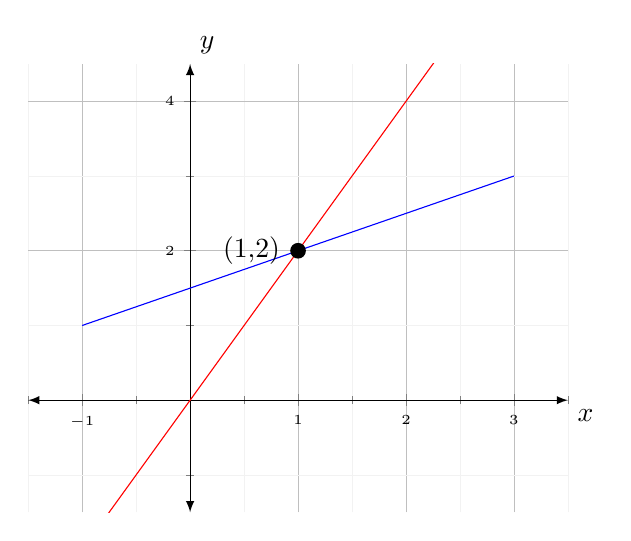
\begin{tikzpicture}
\begin{axis}[
    xlabel={$x$},
    ylabel={$y$},
    xmin=-1, xmax=3,
    ymin=-1, ymax=4,
    grid=both,
    grid style={line width=.1pt, draw=gray!10},
    major grid style={line width=.2pt,draw=gray!50},
    axis lines=middle,
    minor tick num=1,
    enlargelimits={abs=0.5},
    axis line style={latex-latex},
    ticklabel style={font=\tiny},
    xlabel style={at={(ticklabel* cs:1)},anchor=north west},
    ylabel style={at={(ticklabel* cs:1)},anchor=south west}
]

% Lines
\addplot[domain=-1:3, samples=2, red]{2*x};
\addplot[domain=-1:3, samples=2, blue]{(x+3)/2};
% Solution point
\node[label={180:{(1,2)}},circle,fill,inner sep=2pt] at (axis cs:1,2) {};
\end{axis}
\end{tikzpicture}
\end{center}

This graphical representation is known as the \textbf{Row Formulation} of the system.

\subsection*{Column Formulation}

Alternatively, we can express the system in terms of a linear combination of column vectors, known as the \textbf{Column Formulation}.

\begin{equation*}
    x\begin{bmatrix}
        2 \\
        -1
    \end{bmatrix}
    +
    y\begin{bmatrix}
        -1 \\
        2
    \end{bmatrix}
    =
    \begin{bmatrix}
        0 \\
        3
    \end{bmatrix}
\end{equation*}

The weights \( x \) and \( y \) are the scalars that, when used to multiply the respective column vectors and then added together, yield the resultant vector on the right-hand side.

% \subsection*{Geometrical Interpretation}

% The solution \( (x = 1, y = 2) \) represents the point at which the linear combination of the column vectors equals the constant vector:
% \begin{equation*}
%     1\begin{bmatrix}
%         2 \\
%         -1
%     \end{bmatrix}
%     +
%     2\begin{bmatrix}
%         -1 \\
%         2
%     \end{bmatrix}
%     =
%     \begin{bmatrix}
%         0 \\
%         3
%     \end{bmatrix}
% \end{equation*}

% The collection of all possible linear combinations of the column vectors spans the entire 2D plane, which in linear algebra is referred to as the \textbf{span} of the vectors.

\subsection*{Geometrical Representation}

The solution to the system of equations corresponds to the specific linear combination of the column vectors that results in the right-hand side vector.

% The column vectors diagram
\begin{center}
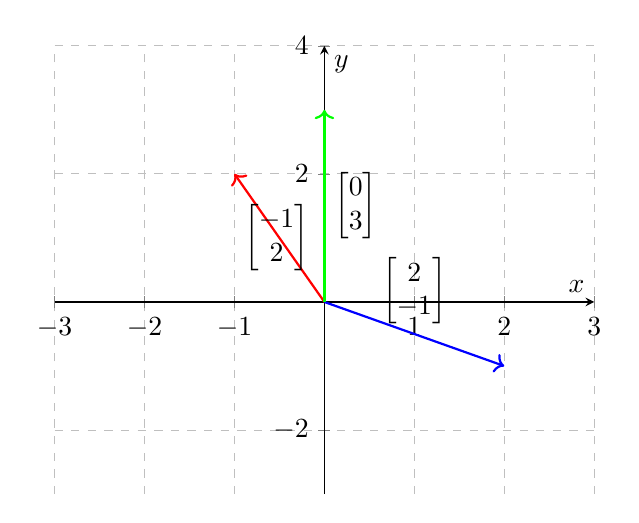
\begin{tikzpicture}
\begin{axis}[
    axis lines=middle,
    xlabel={$x$},
    ylabel={$y$},
    xmin=-3, xmax=3,
    ymin=-3, ymax=4,
    grid=major,
    grid style=dashed,
]

% Vector [2 -1]
\addplot[->, thick, blue] coordinates {(0,0) (2,-1)};
\node[anchor=south] at (axis cs:1,-0.5) {$\begin{bmatrix} 2 \\ -1 \end{bmatrix}$};

% Vector [-1 2]
\addplot[->, thick, red] coordinates {(0,0) (-1,2)};
\node[anchor=west] at (axis cs:-1,1) {$\begin{bmatrix} -1 \\ 2 \end{bmatrix}$};

% Resultant vector [0 3]
\addplot[->, thick, green] coordinates {(0,0) (0,3)};
\node[anchor=west] at (axis cs:0,1.5) {$\begin{bmatrix} 0 \\ 3 \end{bmatrix}$};

\end{axis}
\end{tikzpicture}
\end{center}

The combination of \( x = 1 \) and \( y = 2 \) yields the solution to the system:
\[
1 \begin{bmatrix} 2 \\ -1 \end{bmatrix} + 2 \begin{bmatrix} -1 \\ 2 \end{bmatrix} = \begin{bmatrix} 0 \\ 3 \end{bmatrix}
\]

\begin{center}
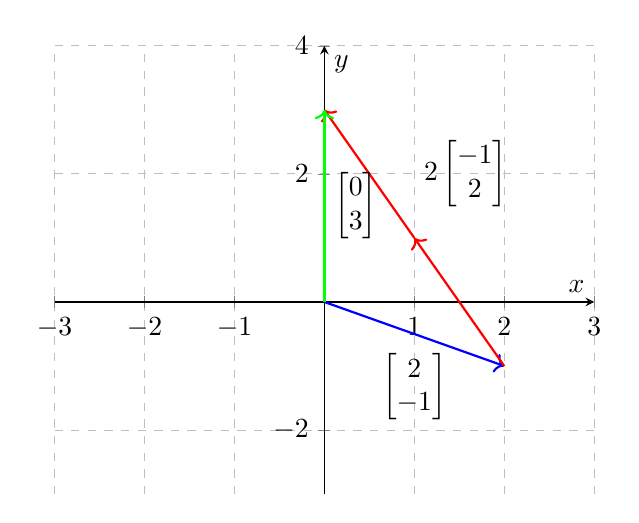
\begin{tikzpicture}
\begin{axis}[
    axis lines=middle,
    xlabel={$x$},
    ylabel={$y$},
    xmin=-3, xmax=3,
    ymin=-3, ymax=4,
    grid=major,
    grid style=dashed,
]

% Vector [2 -1]
\addplot[->, thick, blue] coordinates {(0,0) (2,-1)};
\node[anchor=south] at (axis cs:1,-2) {$\begin{bmatrix} 2 \\ -1 \end{bmatrix}$};

% Vector [-1 2]
\addplot[->, thick, red] coordinates {(2,-1) (1,1)};
\node[anchor=west] at (axis cs:1,2) {$2\begin{bmatrix} -1 \\ 2 \end{bmatrix}$};

\addplot[->, thick, red] coordinates {(1,1) (0,3)};


% Resultant vector [0 3]
\addplot[->, thick, green] coordinates {(0,0) (0,3)};
\node[anchor=west] at (axis cs:0,1.5) {$\begin{bmatrix} 0 \\ 3 \end{bmatrix}$};

\end{axis}
\end{tikzpicture}
\end{center}


\subsection*{Span of Vectors}

The span of a set of vectors is the collection of all possible linear combinations of those vectors. In the case of two non-parallel vectors in 2D space, their span is the entire plane.

% The span of vectors diagram
\begin{center}
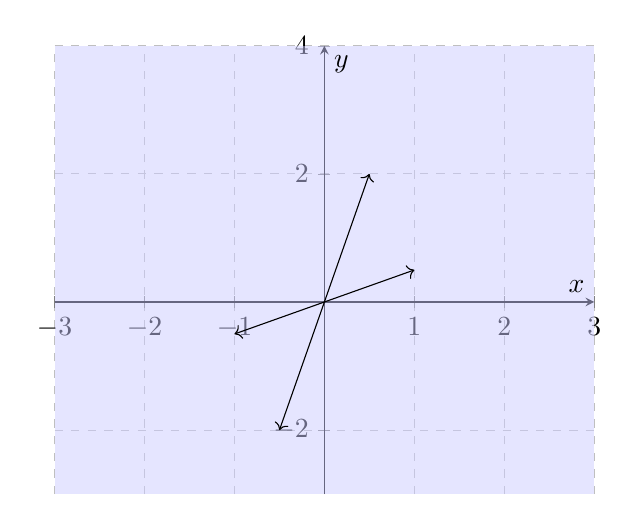
\begin{tikzpicture}
\begin{axis}[
    axis lines=middle,
    xlabel={$x$},
    ylabel={$y$},
    xmin=-3, xmax=3,
    ymin=-3, ymax=4,
    grid=major,
    grid style=dashed,
]

% Span area
\fill[blue!20, opacity=0.5] (axis cs:-3,-3) -- (axis cs:3,-3) -- (axis cs:3,4) -- (axis cs:-3,4) -- cycle;

% Some vectors in the span
\addplot[->, black] coordinates {(0,0) (1,0.5)};
\addplot[->, black] coordinates {(0,0) (-1,-0.5)};
\addplot[->, black] coordinates {(0,0) (0.5,2)};
\addplot[->, black] coordinates {(0,0) (-0.5,-2)};

\end{axis}
\end{tikzpicture}
\end{center}

This illustrates that all possible linear combinations of the columns \( \begin{bmatrix} 2 \\ -1 \end{bmatrix} \) and \( \begin{bmatrix} -1 \\ 2 \end{bmatrix} \) cover the entire 2D plane.


\subsection*{Matrix Formulation}
In matrix formulation we abandon scalar variables and numbers. Every entity is part of either a matrix or a vector as follows:

\begin{equation*}
    \begin{bmatrix}
        2 & -1 \\
        -1 & 2
    \end{bmatrix}
    \begin{bmatrix}
        x \\
        y
    \end{bmatrix}
    =
    \begin{bmatrix}
        0 \\
        3
    \end{bmatrix}
\end{equation*}


We assume we have $m$ equations and $n$ unknowns and can depict the matrix formulation as:

\[\mathbf{Ax} = \mathbf{b}\]

where \textbf{A} is a matrix of size $m\times n$ and \textbf{x} is a column vector of size $m\times 1$.


\subsection*{3D Matrix Example}

Consider the following system of three equations with three unknowns:
\begin{align}
    2x - y &= 0, \\
    -x + 2y - z &= -1, \\
    -3y + 4z &= 4.
\end{align}

This system can be written in matrix form \( \mathbf{A}\mathbf{x} = \mathbf{b} \) as:
\[
\mathbf{A} =
\begin{bmatrix}
    2 & -1 & 0 \\
    -1 & 2 & -1 \\
    0 & -3 & 4
\end{bmatrix},
\quad
\mathbf{b} =
\begin{bmatrix}
    0 \\
    -1 \\
    4
\end{bmatrix}.
\]

In row formulation, each row represents a plane in the 3D space. The solution of the system is where these three planes intersect. Visualising the solution in higher dimensions can be challenging.

% 3D planes intersection diagram
\begin{center}
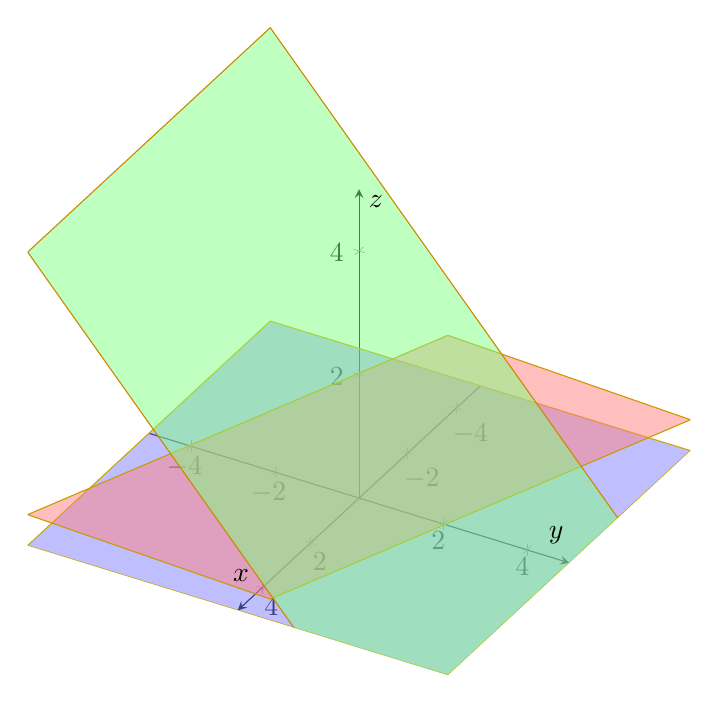
\begin{tikzpicture}
\begin{axis}[
    view={120}{40},
    axis lines=center,
    width=10cm,
    height=10cm,
    xmin=-5,
    xmax=5,
    ymin=-5,
    ymax=5,
    zmin=0,
    zmax=5,
    xlabel={$x$},
    ylabel={$y$},
    zlabel={$z$},
    grid=major,
    grid style={dashed, gray!30},
]

% Planes
\addplot3[surf, fill opacity=0.5, fill=blue!50, domain=-5:5, domain y=-5:5, samples=2, samples y=2] {0};
\addplot3[surf, fill opacity=0.5, fill=red!50, domain=-5:5, domain y=-5:5, samples=2, samples y=2] {(1/2)*x + (1/2)*y + 1/2};
\addplot3[surf, fill opacity=0.5, fill=green!50, domain=-5:5, domain y=-5:5, samples=2, samples y=2] {(-3/4)*y + 1};

\end{axis}
\end{tikzpicture}
\end{center}


In column formulation, the system is viewed as a combination of column vectors scaled by the unknowns:
\[
x \begin{bmatrix} 2 \\ -1 \\ 0 \end{bmatrix} +
y \begin{bmatrix} -1 \\ 2 \\ -3 \end{bmatrix} +
z \begin{bmatrix} 0 \\ -1 \\ 4 \end{bmatrix} =
\begin{bmatrix} 0 \\ -1 \\ 4 \end{bmatrix}.
\]



\begin{center}
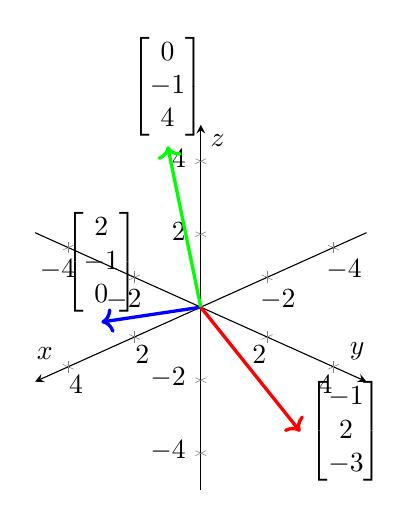
\begin{tikzpicture}
\begin{axis}[
    width=10cm,
    height=10cm,
    view={135}{30},
    axis lines=center,
    xlabel={$x$},
    ylabel={$y$},
    zlabel={$z$},
    xmin=-5,
    xmax=5,
    ymin=-5,
    ymax=5,
    zmin=-5,
    zmax=5,
    grid=major,
    grid style={dashed, gray!30},
]

% Vector [2 -1 0]
\addplot3[->, blue, very thick] coordinates {(0,0,0) (2,-1,0)};
\node[anchor=south] at (axis cs:2,-1,0) {$\begin{bmatrix} 2 \\ -1 \\ 0 \end{bmatrix}$};

% Vector [-1 2 -3]
\addplot3[->, red, very thick] coordinates {(0,0,0) (-1,2,-3)};
\node[anchor=west] at (axis cs:-1,2,-3) {$\begin{bmatrix} -1 \\ 2 \\ -3 \end{bmatrix}$};

% Vector [0 -1 4]
\addplot3[->, green, very thick] coordinates {(0,0,0) (0,-1,4)};
\node[anchor=south] at (axis cs:0,-1,4) {$\begin{bmatrix} 0 \\ -1 \\ 4 \end{bmatrix}$};

\end{axis}
\end{tikzpicture}
\end{center}

The solution is the particular combination of column vectors that yield the right-hand side vector. For the given system, the solution is \(\mathbf{x} = \begin{bmatrix} 0 \\ 0 \\ 1 \end{bmatrix}\).
\begin{itemize}
    \item The solutions of a system of three equations with three unknowns lie within the 3D space. 
    \item A matrix \( \mathbf{A} \) is invertible if its column vectors are linearly independent, meaning they do not lie in the same plane. 
    \item If at least one column is a linear combination of the others, the matrix is not invertible, and the system may not have a unique solution for every \( \mathbf{b} \) in \( \mathbb{R}^3 \).
\end{itemize}



The concept of row and column formulations leads to the broader idea of vector spaces. Before delving deeper into vector spaces, it is essential to understand practical algorithms to solve systems of linear equations, such as Gaussian elimination.


\section{Gaussian Elimination}

Gaussian Elimination, also known as Row Reduction, is a systematic method for solving systems of linear equations. It involves performing operations on the rows of the augmented matrix of the system to obtain a row-echelon form, from which the solutions can easily be determined through back-substitution.

\subsection*{Example System}

Consider the system of linear equations:
\begin{align}
    x + 2y + z &= 2, \\
    3x + 8y + z &= 12, \\
    4y + z &= 2.
\end{align}

\subsection*{Row Reduction Process}

\textbf{Step 1:} Eliminate \( x \) from the second and third equations.

We multiply the first equation by 3 and subtract it from the second to eliminate \( x \):
\[
\begin{aligned}
    [2] - 3[1]: & \quad (3x + 8y + z) - 3( x + 2y + z) = 12 - 6, \\
    & \quad 2y - 2z = 6.
\end{aligned}
\]

\textbf{Step 2:} Multiply the first equation by 2 and subtract it from the third to eliminate \( x \):
\[
\begin{aligned}
    [3] - 2[1]: & \quad (4y + z) - 2( x + 2y + z)  = 2-2(2) , \\
    & \quad 5z = -10.
\end{aligned}
\]

\textbf{Step 3:} Now, we have a new system of equations:
\begin{align}
    x + 2y + z &= 2, \\
     2y - 2z &= 6, \\
    5z &= -10.
\end{align}

\textbf{Step 4:} We have achieved an upper triangular matrix.

\subsection*{Back-Substitution}

Once the matrix is in upper triangular form, we can find the solutions by back-substitution. The final form of the matrix and the solutions are:
\begin{align}
    x + 2y + z &= 2, \\
    2y - 2z &= 6, \\
    5z &= -10,
\end{align}

Since the system of equations is now in upper triangular form, we can solve the equations in reverse order. This method is straightforward because each equation can be solved for one variable at a time, starting from the last equation.\\


We start by solving the last equation for \( z \):
\begin{align*}
    5z &= -10 \\
    z &= \frac{-10}{5} \\
    z &= -2.
\end{align*}


Substituting \( z \) into the second equation, we solve for \( y \):
\begin{align*}
    2y - 2(-2) &= 6 \\
    2y + 4 &= 6 \\
    2y &= 6 - 4 \\
    2y &= 2 \\
    y &= \frac{2}{2} \\
    y &= 1.
\end{align*}


Finally, we substitute \( y \) and \( z \) back into the first equation to solve for \( x \):
\begin{align*}
    x + 2(1) - 2 &= 2 \\
    x + 2 - 2 &= 2 \\
    x &= 2 - 2 + 2 \\
    x &= 2.
\end{align*}



The solution to the system is:
\begin{align*}
    x &= 2, \\
    y &= 1, \\
    z &= -2.
\end{align*}





We solve the equations in reverse order because the system after elimination is triangular, allowing us to express each variable in terms of the subsequent ones.


\subsection*{Matrix Transformation}

The original matrix \( \mathbf{A} \) is:
\[
\mathbf{A} =
\begin{bmatrix}
    1 & 2 & 1 \\
    3 & 8 & 1 \\
    0 & 4 & 1
\end{bmatrix}.
\]

After applying the row operations \([2] - 3[1]\) and \([3] - 2[2]\), the matrix is transformed into:
\[
\mathbf{U} =
\begin{bmatrix}
    \boxeditem{1} & 2 & 1 \\
    0 & \boxeditem{2} & -2 \\
    0 & 0 & \boxeditem{5}
\end{bmatrix},
\]
where the elements in the diagonal of \( \mathbf{U} \) are called \textit{pivots}.

\subsection*{Column Transformation}

Similarly, the column vector \( \mathbf{b} \) is transformed alongside matrix \( \mathbf{A} \) as follows:
\[
\mathbf{b} =
\begin{bmatrix}
    2 \\
    12 \\
    2
\end{bmatrix}
\rightarrow
\begin{bmatrix}
    2 \\
    6 \\
    -10
\end{bmatrix}.
\]

\subsection*{Augmented Matrix}

It is often convenient to combine the matrix \( \mathbf{A} \) and the vector \( \mathbf{b} \) into an augmented matrix \( [ \mathbf{A} | \mathbf{b} ] \) and perform row operations on this combined matrix:
\[
[\mathbf{A}|\mathbf{b}] =
\left[
\begin{array}{ccc|c}
    1 & 2 & 1 & 2 \\
    3 & 8 & 1 & 12 \\
    0 & 4 & 1 & 2
\end{array}
\right]
\rightarrow
\left[
\begin{array}{ccc|c}
    1 & 2 & 1 & 2 \\
    0 & 2 & -2 & 6 \\
    0 & 0 & 5 & -10
\end{array}
\right].
\]

This augmented matrix represents the system after the row operations have been applied, and it is now ready for back-substitution to solve for the unknowns.



\section{LU Decomposition}

The process of Gaussian Elimination can be represented algebraically using matrices. Specifically, each elementary row operation can be performed by multiplying the matrix of coefficients by an \textit{elimination matrix}.

\subsection*{Transformation of Matrix A}

Consider the system of linear equations represented in matrix form by \( \mathbf{A}\mathbf{x} = \mathbf{b} \). The coefficient matrix \( \mathbf{A} \) is transformed through the elimination process as follows:

\[
\mathbf{A} =
\begin{bmatrix}
    1 & 2 & 1 \\
    3 & 8 & 1 \\
    0 & 4 & 1
\end{bmatrix}
\quad \underrightarrow{\text{[2] - 3[1]}}
\quad
\begin{bmatrix}
    1 & 2 & 1 \\
    0 & 2 & -2 \\
    0 & 4 & 1
\end{bmatrix}
\quad \underrightarrow{\text{[3] - 2[2]}}
\quad
\begin{bmatrix}
    1 & 2 & 1 \\
    0 & 2 & -2 \\
    0 & 0 & 5
\end{bmatrix} = \mathbf{U}
\]

\subsection*{Elimination Matrices}

Each step where a substitution of the form \([i] + c \times [j]\) is performed corresponds to multiplying the current matrix by an identity matrix with its \(i,j\) element replaced by \(c\). This special matrix is denoted \(E_{ij}\).

For instance, the first step \([2] - 3[1]\) can be represented by an elimination matrix \(E_{21}\):
\[
E_{21} =
\begin{bmatrix}
    1 & 0 & 0 \\
    -3 & 1 & 0 \\
    0 & 0 & 1
\end{bmatrix}
\]

\subsection*{Matrix Multiplication Representation}

The second step of elimination, \([3] - 2[2]\), can be represented as:
\[
E_{32} =
\begin{bmatrix}
    1 & 0 & 0 \\
    0 & 1 & 0 \\
    0 & -2 & 1
\end{bmatrix}
\]

Applying these elimination matrices to \( \mathbf{A} \) sequentially gives us \( \mathbf{U} \):
\[
E_{32}(E_{21}\mathbf{A}) = \mathbf{U}
\]
The brackets can be dropped due to the associative property of matrix multiplication, thus:
\[
E_{32}E_{21}\mathbf{A} = \mathbf{U}
\]

\subsection*{Inverses of Elimination Matrices}

The inverse of an elimination matrix \(E_{ij}\) is conveniently obtained by changing the sign of its non-zero off-diagonal element. For example:
\[
E_{21}^{-1} =
\begin{bmatrix}
    1 & 0 & 0 \\
    3 & 1 & 0 \\
    0 & 0 & 1
\end{bmatrix}
\quad \text{and} \quad
E_{32}^{-1} =
\begin{bmatrix}
    1 & 0 & 0 \\
    0 & 1 & 0 \\
    0 & 2 & 1
\end{bmatrix}
\]

The inverses of these matrices reverse the elimination steps, providing a method to return to the original matrix \( \mathbf{A} \).

LU decomposition is a method where a matrix \( \mathbf{A} \) is factorized into two matrices, \( \mathbf{L} \) and \( \mathbf{U} \), where \( \mathbf{L} \) is a lower triangular matrix and \( \mathbf{U} \) is an upper triangular matrix. This factorization is particularly useful for solving systems of equations, inverting matrices, and computing determinants.

\subsection*{Matrix Factorization}

The elimination process can be expressed as a sequence of matrix multiplications, transforming the original matrix \( \mathbf{A} \) into an upper triangular matrix \( \mathbf{U} \):
\[
E_{32}E_{21}\mathbf{A} = \mathbf{U}
\]

\subsection*{Inversion of Elimination Matrices}

By sequentially multiplying both sides from the left with the inverses of the elimination matrices in reverse order, we can express \( \mathbf{A} \) as:
\[
\mathbf{A} = E_{21}^{-1}E_{32}^{-1}\mathbf{U}
\]

\subsection*{Constructing Matrix L}

The product of the inverses of the elimination matrices gives us matrix \( \mathbf{L} \):
\[
\mathbf{L} = E_{21}^{-1}E_{32}^{-1} = \begin{bmatrix}
    1&0&0\\3&1&0\\0&2&1
\end{bmatrix}
\]
Matrix \( \mathbf{L} \) has the nice property that its elements below the diagonal are the multipliers used in the elimination process.

\subsection*{LU Decomposition}

Thus, matrix \( \mathbf{A} \) can be decomposed as:
\[
\mathbf{A} = \mathbf{L}\mathbf{U}
\]
This is the LU decomposition of \( \mathbf{A} \).

\subsection*{Permutation Matrix}

In the general case where row exchanges are required during the elimination process, we introduce a permutation matrix \( \mathbf{P} \). The PA = LU factorization incorporates these permutations:
\[
\mathbf{P}\mathbf{A} = \mathbf{L}\mathbf{U}
\]
A permutation matrix \( \mathbf{P} \) arises from the identity matrix if we reorder the rows to ensure that the pivot elements are non-zero.

\subsection*{Example of a Permutation Matrix}

For instance, if we need to swap rows 1 and 2 in matrix \( \mathbf{A} \) to get a non-zero pivot in the first position, the permutation matrix \( \mathbf{P}_{12} \) and the operation would look like this:
\[
\mathbf{P}_{12} =
\begin{bmatrix}
    0 & 1 & 0 \\
    1 & 0 & 0 \\
    0 & 0 & 1
\end{bmatrix}
\quad \text{and} \quad
\mathbf{P}_{12}\mathbf{A} =
\begin{bmatrix}
    0 & 1 & 0 \\
    1 & 0 & 0 \\
    0 & 0 & 1
\end{bmatrix}
\begin{bmatrix}
    1 & 2 & 1 \\
    3 & 8 & 1 \\
    0 & 4 & 1
\end{bmatrix}
=
\begin{bmatrix}
    3 & 8 & 1 \\
    1 & 2 & 1 \\
    0 & 4 & 1
\end{bmatrix}
\]

This reordering is essential to avoid dividing by zero when attempting to use that pivot to eliminate the variables in the column below.

\begin{definitionbox}{General LU Decomposition}

For any invertible matrix \( \mathbf{A} \), the LU decomposition with partial pivoting (where row exchanges are accounted for) can be expressed as:
\[
\mathbf{PA} = \mathbf{LU}
\]
Here, \( \mathbf{P} \) is the permutation matrix that records the row exchanges, \( \mathbf{L} \) is the product of the inverses of the elimination matrices (lower triangular), and \( \mathbf{U} \) is the resulting upper triangular matrix after applying Gaussian elimination.


The complete LU decomposition with a permutation matrix is thus represented as:
\[
\mathbf{A} = \mathbf{P}^{-1}\mathbf{L}\mathbf{U}
\]
It is important to note that \( \mathbf{P}^{-1} = \mathbf{P}^\mathsf{T} \) since permutation matrices are orthogonal.

\end{definitionbox}


\section{Vector Spaces, Inner Product and Norm}
We need to define a common framework to handle vectors in dimensions $\leq 3$ (geometry is useful) and in dimensions $> 3$.

\begin{definitionbox}{Vector Space}    
A vector space is a collection of vectors that form a nonempty set $E$ with two operations: addition and scalar multiplication that satisfy the following properties:

\begin{itemize}
    \item \textbf{Commutativity:} For all \( x, y \in E \), we have \( x + y = y + x \).
    \item \textbf{Associativity:} For all \( x, y, z \in E \), we have \( (x + y) + z = x + (y + z) \).
    \item \textbf{Distributivity:} For all \( x \in E \) and scalars \( \alpha, \beta \), we have \( (\alpha + \beta) x = \alpha x + \beta x \) and \( \alpha(x + y) = \alpha x + \alpha y \).
    \item \textbf{Existence of Inverses:} For every \( x, y \in E \) there exists \( z \in E \) such that \( x + z = y \).
    \item \textbf{Compatibility of Scalars and Multiplication:} For scalars \( \alpha, \beta \) and all \( x \in E \), we have \( \alpha(\beta x) = (\alpha\beta)x \).
    \item \textbf{Identity Element:} There exists an identity element \( 1 \) such that for every \( x \in E \), we have \( 1x = x \).
\end{itemize}
\end{definitionbox}

\begin{definitionbox}{Inner Product}
Let \( E \) be a complex vector space. A mapping \( \langle \cdot, \cdot \rangle \) from \( E \times E \rightarrow \mathbb{C} \) is called an inner product in \( E \) if for any \( x, y, z \in E \) and \( \alpha, \beta \in \mathbb{C} \) the following conditions are satisfied:
\begin{itemize}
    \item \textbf{Conjugate Symmetry:} \( \langle x, y \rangle = \overline{\langle y, x \rangle} \).
    \item \textbf{Linearity in the first argument:} \( \langle \alpha x + \beta y, z \rangle = \alpha \langle x, z \rangle + \beta \langle y, z \rangle \).
    \item \textbf{Positive-definiteness:} \( \langle x, x \rangle \geq 0 \) and \( \langle x, x \rangle = 0 \) implies \( x = 0 \).
\end{itemize}

In $\mathbb{C}$, the standard inner product between components of vectors $a, b \in \mathbb{C}^n$ can be written as 

\begin{equation}
\sum^n_{i=1}a_i \bar{b}_i    
\end{equation}

Where $\bar{b_i}$ is the complex conjugate of $b_i$.

\end{definitionbox}

\begin{definitionbox}{Norm}
It is always useful to be able to determine the size of an object, in the case of vector spaces this is achieved using the notion of ‘norm’.\\ 
A norm on a vector space \( E \) over \( \mathbb{C} \) (or \( \mathbb{R} \)) is a real-valued function with the following properties for any \( x, y \in E \) and \( \alpha \in \mathbb{C} \):
\begin{itemize}
    \item \textbf{Positive definiteness:} \( \|x\| \geq 0 \), and \( \|x\| = 0 \) if and only if \( x = 0 \).
    \item \textbf{Homogeneity Property:} \( \|\alpha x\| = |\alpha| \|x\| \).
    \item \textbf{Triangle Inequality:} \( \|x + y\| \leq \|x\| + \|y\| \).
\end{itemize}
Given the definition of inner product, we define the induced norm of a vector \( x \) as:
\[ \|x\|_2 = \sqrt{\langle x, x \rangle}  = \sqrt{\sum^n_{i=1}|x_i|^2}\]

The more general norm is defined as:
\[ \|x\|_p = \sqrt{\langle x, x \rangle}  = \left(\sum^n_{i=1}|x_i|^p\right) ^{\frac{1}{p}}\]

\end{definitionbox}


\subsection*{Examples of Vector Spaces}
\textbf{n-dimensional Vectors in \( \mathbb{R}^n \) or \( \mathbb{C}^n \)}\\
A vector is a set of scalars placed jointly in a vertical fashion (column vector).
\begin{itemize}
    \item A column vector of size \( n \) is denoted as \( \mathbf{x} = \begin{bmatrix} x_1 \\ x_2 \\ \vdots \\ x_n \end{bmatrix} \).
    \item The Hermitian transpose of \( \mathbf{x} \) is a row vector of size \( n \) denoted as \( \mathbf{x}^H = (x_1^* \ x_2^* \ \cdots \ x_n^*) \).
    \item Addition and product with a scalar are easily defined, while the inner product is: \( \langle \mathbf{x}, \mathbf{y} \rangle = \mathbf{y}^H \mathbf{x} = \sum_{i=1}^{n} x_i y_i^* \).
    \item Consequently, the induced norm is: \( \|\mathbf{x}\| = \sqrt{\langle \mathbf{x}, \mathbf{x} \rangle} = \left( \sum_{i=1}^{n} |x_i|^2 \right)^{1/2} \).
\end{itemize}
\textbf{Matrices of size \( m \times n \)}\\
The space of matrices of size \( m \times n \), that is, the space with elements \( A \in \mathbb{C}^{m \times n} \) includes:
\begin{itemize}
    \item Matrices are typically used to model linear equations but are more complex objects.
    \item The inner product of two matrices \( A, B \) is the element-by-element product: \( \langle A, B \rangle = \sum_{i,j} a_{i,j} b_{i,j}^* \).
    \item This leads to the induced norm (Frobenius norm): \( \|A\|_F = \sqrt{\sum_{i,j} |a_{i,j}|^2} \).
    \item More general norms: \( \|A\|_p = \sup_{\|x\|_p \neq 0} \frac{\|Ax\|_p}{\|x\|_p} \).
\end{itemize}

\newpage
\section*{On the Notion of the Norm}

\subsection*{Unit-norm Vectors for Different p-norms}

\begin{center}
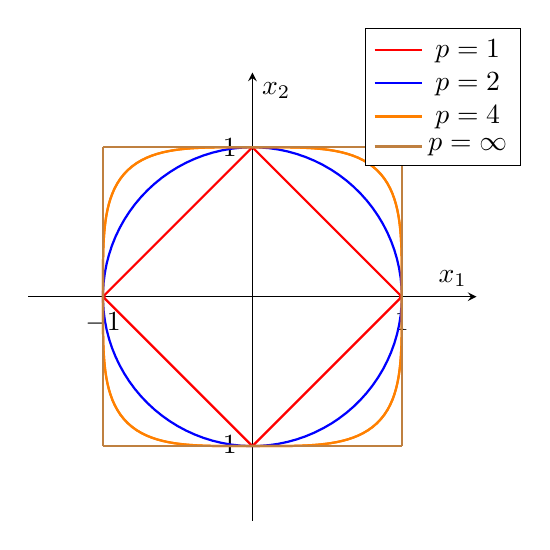
\begin{tikzpicture}
\begin{axis}[
    axis lines=middle,
    xlabel=\(x_1\),
    ylabel=\(x_2\),
    xmin=-1.5, xmax=1.5,
    ymin=-1.5, ymax=1.5,
    axis equal image,
    legend style={at={(1.1,1.1)},anchor=north east}
]

% Legend entries
\addlegendimage{red, thick}
\addlegendentry{\(p=1\)}
\addlegendimage{blue, thick}
\addlegendentry{\(p=2\)}
\addlegendimage{orange, thick}
\addlegendentry{\(p=4\)}
\addlegendimage{brown, thick}
\addlegendentry{\(p=\infty\)}

% 1-norm (diamond shape)
\addplot [red, thick, domain=-1:1, samples=100] ({1-abs(x)},x);
\addplot [red, thick, domain=-1:1, samples=100] ({-1+abs(x)},x);

% 2-norm (circle)
\addplot [blue, thick, domain=0:360, samples=100] ({cos(x)},{sin(x)});

% 4-norm
\addplot [orange, thick, domain=0:360, samples=100, variable=\t] 
    ({(cos(t)^(4) + sin(t)^(4))^(-1/4)*cos(t)}, {(cos(t)^(4) + sin(t)^(4))^(-1/4)*sin(t)});
\addplot [orange, thick, domain=0:360, samples=100, variable=\t] 
    ({-(cos(t)^(4) + sin(t)^(4))^(-1/4)*cos(t)}, {-(cos(t)^(4) + sin(t)^(4))^(-1/4)*sin(t)});

% Infinity norm (square)
\addplot [brown, thick, domain=-1:1] ({1},x);
\addplot [brown, thick, domain=-1:1] ({-1},x);
\addplot [brown, thick, domain=-1:1] (x,{1});
\addplot [brown, thick, domain=-1:1] (x,{-1});

\end{axis}
\end{tikzpicture}
\end{center}




Note: In this plot, the \( p \)-norm is defined for a unit vector \( x \) in \( \mathbb{R}^2 \) as \( \|x\|_p = \left( |x_1|^p + |x_2|^p \right)^{1/p} \), where \( p \) takes values of 1, 2, 4, \( \infty \), for the plotted shapes. Note that $p$ cannot take on non-integer values.


\section{Cauchy-Schwarz Inequality}


The Cauchy-Schwarz Inequality is a fundamental result in vector analysis which provides a bound for the absolute value of the inner product of two vectors.

\subsection{Introduction}
For all vectors \( \mathbf{x}, \mathbf{y} \) in an inner-product space, the following inequality holds:
\[ |\langle \mathbf{x}, \mathbf{y} \rangle| \leq \|\mathbf{x}\| \|\mathbf{y}\| \]


This inequality allows us to estimate the similarity of two vectors and to introduce the idea of direction. It is particularly useful in defining the angle between two vectors:
\[ \cos \theta = \frac{\langle \mathbf{x}, \mathbf{y} \rangle}{\|\mathbf{x}\| \|\mathbf{y}\|} \]

Two vectors are considered 'maximally' similar when one is a rescaled version of the other, and they are 'maximally' dissimilar, or orthogonal, when \( \theta = \frac{\pi}{2} \), that is, when \( \langle \mathbf{x}, \mathbf{y} \rangle = 0 \). If the vectors are orthogonal and their magnitudes are 1, they are called orthonormal.

\subsection{Proof of the Cauchy-Schwarz Inequality}

\textit{Sketch of the proof:}
Starting from the non-negativity of the norm, we have:
\[ 0 \leq \|\mathbf{x} - \alpha \mathbf{y}\|^2 = \langle \mathbf{x} - \alpha \mathbf{y}, \mathbf{x} - \alpha \mathbf{y} \rangle \]
Expanding the inner product, we get:
\[ = \|\mathbf{x}\|^2 - \langle \mathbf{x}, \alpha \mathbf{y} \rangle - \langle \alpha \mathbf{y}, \mathbf{x} \rangle + |\alpha|^2 \|\mathbf{y}\|^2 \]

Choosing \( \alpha = \frac{\langle \mathbf{x}, \mathbf{y} \rangle}{\|\mathbf{y}\|^2} \) and using the property that if \( c = \langle \mathbf{x}, \mathbf{y} \rangle \) then \( \langle \mathbf{y}, \mathbf{x} \rangle = c^* \), we obtain:
\[ 0 \leq \|\mathbf{x}\|^2 - \frac{|\langle \mathbf{x}, \mathbf{y} \rangle|^2}{\|\mathbf{y}\|^2} \]

Which simplifies to the Cauchy-Schwarz inequality:
\[ |\langle \mathbf{x}, \mathbf{y} \rangle|^2 \leq \|\mathbf{x}\|^2 \|\mathbf{y}\|^2 \]
And taking the square root of both sides gives us the final form of the inequality.

% \section{Linear Combination and Linear Independence}
\section{Linear Mappings, Basis and Dimension}

Let \( v_1, v_2, \ldots, v_n \) be vectors in a vector space of dimension \( n \). For scalar coefficients \( c_i \in \mathbb{R} \), the linear combination \( x \) can be expressed as:
    \[ x = c_1v_1 + c_2v_2 + \ldots + c_nv_n \]
    In matrix/vector form, this is represented as:
    \[
    x = \begin{bmatrix}
    v_{1,1} & v_{1,2} & \cdots & v_{1,n} \\
    v_{2,1} & v_{2,2} & \cdots & v_{2,n} \\
    \vdots & \vdots & \ddots & \vdots \\
    v_{n,1} & v_{n,2} & \cdots & v_{n,n}
    \end{bmatrix}
    \begin{bmatrix}
    c_1 \\
    c_2 \\
    \vdots \\
    c_n
    \end{bmatrix}
    \]

\begin{itemize}
    \item The vectors \( v_1, v_2, \ldots, v_n \) are \textbf{independent} if no linear combination of them gives the zero vector (except the trivial combination where all \( c_i = 0 \)).

    \item Two non-zero, non-parallel vectors in two-dimensional space are independent because no scalar multiples of one can be added to obtain the other.

    \item Considering three vectors in the two-dimensional space, they are \textbf{dependent} if there exists non-trivial scalars \( x_i \) such that:
    \[ x_1v_1 + x_2v_2 + x_3v_3 = 0 \]
    This means at least one vector is a linear combination of the others.
\end{itemize}

\subsection{Span}

\begin{definitionbox}{Span}
Let \( T \) be a set of vectors in a vector space \( E \). The \textbf{span} of \( T \), denoted \( \text{span}(T) \), is the set of all vectors that can be expressed as linear combinations of the vectors in \( T \). Formally, for \( V = \text{span}(T) \), any vector \( x \in V \) can be written as:
\[ x = \sum_{i} c_i v_i \]
where \( c_i \in \mathbb{R} \) and \( v_i \in T \). By construction, \( V \) is itself a vector space, and since \( V \subseteq E \), it is a subspace of \( E \).
\end{definitionbox}

\textbf{Example:} The span of two linearly independent vectors in \( \mathbb{R}^3 \) forms a plane, which is a subspace of \( \mathbb{R}^3 \).

\textit{Question:} Is the following plane a subspace as well?
\[ V = \{ x \in \mathbb{R}^3 : x_1 + x_2 + x_3 = 1 \} \]
To be a subspace, \( V \) must include the zero vector and be closed under addition and scalar multiplication. Since the sum of the components must equal 1, \( V \) does not include the zero vector and thus is not a subspace.

\subsection{Basis and Dimension}

\begin{definitionbox}{Vector Space Basis} A \textit{basis} for a vector space \( E \) is a set of vectors \( T \) that are linearly independent and span \( E \). The number of vectors in the basis is called the \textit{dimension} of \( E \).
\end{definitionbox}

\textbf{Example:} The standard basis for \( \mathbb{R}^n \) or \( \mathbb{C}^n \) consists of vectors \( e_i \), where each \( e_i \) has a 1 in the \( i \)-th position and 0s elsewhere. This basis is known as the \textit{canonical basis}.

When a basis also satisfies \( \langle v_i, v_j \rangle = 0 \) for \( i \neq j \), it is called an \textit{orthogonal basis}. If additionally \( \langle v_i, v_i \rangle = 1 \), it is an \textit{orthonormal basis}.

\textbf{Exercise:} Consider \( S = \{(1,2,\gamma)^T : \gamma \in \mathbb{R}\} \subset \mathbb{R}^3 \). The dimension of \( \text{span}(S) \) is 2, as \( S \) can be expressed as the span of \( \{(1,2,0)^T, (0,0,1)^T\} \), which are linearly independent.

\subsection{Orthogonal (Unitary) Matrices}

An \textit{orthonormal basis} of \( n \)-dimensional space can be formed into a matrix \( A \) that is orthogonal (unitary in the complex case). Such a matrix preserves the inner product and, consequently, the induced norm.

\subsubsection*{Properties of Orthogonal Matrices:}
\begin{itemize}
    \item For matrix \( A \) with orthonormal vectors as columns, \( A^HA = AA^H = I \), where \( I \) is the identity matrix, indicating \( A^H = A^{-1} \).
    \item Orthogonal matrices preserve the induced norm: \( \|Ax\|_2 = \|x\|_2 \).
    \item The process to orthogonalize a set of vectors is known as the \textit{Gram-Schmidt process}.
\end{itemize}

\subsubsection*{Examples of Orthogonal Matrices}

\textbf{Rotation Matrices:}
A rotation matrix in 2D is defined by \( Q = \begin{bmatrix} \cos \theta & -\sin \theta \\ \sin \theta & \cos \theta \end{bmatrix} \), which satisfies \( QQ^T = Q^TQ = I \).

\textbf{Permutation Matrices:}
Permutation matrices, such as \( P = \begin{bmatrix} 0 & 1 \\ 1 & 0 \end{bmatrix} \), reorder the rows of the identity matrix. They satisfy \( PQ = QP = I \).

\subsubsection*{Orthogonal Subspaces}

Extending the concept of orthogonality to subspaces requires every vector in one subspace to be orthogonal to every vector in the other subspace.

\begin{definitionbox}{Orthogonality} 
Two subspaces \( V \) and \( W \) of \( E \) are orthogonal if every vector \( v \in V \) is orthogonal to every vector \( w \in W \): \( \langle v, w \rangle = 0 \).
\end{definitionbox}

\begin{definitionbox}{Subspaces} 
The \textit{orthogonal complement} to a subspace \( V \subset E \), denoted \( V^\perp \), is the set of all vectors in \( E \) that are orthogonal to every vector in \( V \).
\end{definitionbox}


\section{Applications}
\subsection{Linear Mappings and Matrices}

\begin{itemize}
    \item We initially thought of matrices and vectors as a means to express linear equations in a compact form. Now, with a deeper understanding of vector spaces, we aim to interpret matrices more `geometrically'.
    \item Matrices facilitate the description of linear transformations between vector spaces. These transformations map vectors from one space, known as the domain, to another, known as the range.
\end{itemize}

\subsection{Understanding Matrix Operations through Linear Mappings}

Assume vector spaces \( X, Y \in \mathbb{R}^2 \), and consider a linear mapping represented by matrix \( A \) such that \( y = Ax \) with:

\[ A = \begin{bmatrix} \cos \theta & -\sin \theta \\ \sin \theta & \cos \theta \end{bmatrix} \]

This matrix \( A \) corresponds to a rotation by an angle \( \theta \) in the 2-dimensional Euclidean space.

\begin{itemize}
    \item To describe a rigid rotation in 3-D, we use rotation matrices that depend on the axis of rotation. For example, rotation about the \( z \)-axis by an angle \( \theta \) is represented by a similar trigonometric matrix with the addition of a third dimension.
    \item A 2-D rotation by \( 2\theta \) can be achieved by multiplying two matrices of rotation by \( \theta \), exploiting the property that matrix multiplication is associative.
    \item To invert a 2-D rotation by \( \theta \), we can either transpose the rotation matrix (since rotation matrices are orthogonal) or construct a new rotation matrix with angle \( -\theta \), effectively rotating in the opposite direction.
\end{itemize}




\subsection{Signal Processing}
Many important operations in signal processing can be describe using matrices.



\subsubsection*{Time-Reversal of Signals}
Given a discrete-time signal \( \mathbf{x} = (x_1, x_2, \ldots, x_n)^T \), its time-reversed version \( \mathbf{y}  = (x_n, \cdots, x_2, x_1)^T\) can be described by:
\[ \mathbf{y} = R\mathbf{x} \]
where \( R \) is the time-reversal matrix, a square matrix with 1's on its anti-diagonal and 0's elsewhere:
\[ R = \begin{bmatrix}
0 & \cdots & 0 & 1 \\
0& \cdots & 1 & 0 \\
\vdots  & \iddots & \vdots & \vdots \\
1 & \cdots & 0 & 0
\end{bmatrix} 
\quad R\mathbf{x} = \begin{bmatrix}
0 & \cdots & 0 & 1 \\
0& \cdots & 1 & 0 \\
\vdots  & \iddots & \vdots & \vdots \\
1 & \cdots & 0 & 0
\end{bmatrix} \begin{bmatrix}
    x_1 \\ x_2 \\ \vdots \\ x_n \\ 
\end{bmatrix} =\begin{bmatrix}
    x_n \\ \vdots \\ x_2 \\ x_1 \\ 
\end{bmatrix}   \]

\subsubsection*{Truncation of Signals}
Given a discrete-time signal \( \mathbf{x} = (x_1, x_2, \ldots, x_n)^T \), to truncate the last \( m-n \) terms of a signal with \(m<n\), use a truncation matrix \( T \) of size \( m \times n \) with 1's on the diagonal (the left part is a $mxm$ identity matrix) and 0's elsewhere:
\[ T = \begin{bmatrix}
1 & 0 & \cdots & 0 & 0&\cdots & 0 \\
0 & 1 & \cdots & 0 & 0&\cdots & 0 \\
\vdots & \vdots & \ddots & \vdots & \vdots&\cdots & \vdots \\
0 & 0 & \cdots & 1 & 0&\cdots & 0
\end{bmatrix} \]
Then \( \mathbf{y} = T\mathbf{x} \).

\[
\mathbf{y}=\begin{bmatrix}
1 & 0 & \cdots & 0 & 0&\cdots & 0 \\
0 & 1 & \cdots & 0 & 0&\cdots & 0 \\
\vdots & \vdots & \ddots & \vdots & \vdots&\cdots & \vdots \\
0 & 0 & \cdots & 1 & 0&\cdots & 0
\end{bmatrix} \begin{bmatrix}
    x_1 \\ x_2 \\ \vdots \\ x_m \\ x_{m+1} \\ \vdots \\ x_n
\end{bmatrix}= \begin{bmatrix}
    x_1 \\ x_2 \\ \vdots \\ x_m \\ 
\end{bmatrix} 
\]

\subsubsection*{Zero-Padding Operation}
Zero-padding a signal \( \mathbf{x} \) to length \( m > n \) can be done using an extension matrix \( E \) of size \( m \times n \). The zero-padded signal is \( \mathbf{y} = E\mathbf{x} \).
\[ E = \begin{bmatrix}
1 & 0 & \cdots & 0 \\
0 & 1 & \cdots & 0 \\
\vdots & \vdots & \ddots & \vdots \\
0 & 0 & \cdots & 1 \\
0 & 0 & \cdots & 0 \\
\vdots & \vdots & \ddots & \vdots \\
0 & 0 & \cdots & 0
\end{bmatrix}\quad E\mathbf{x}= \begin{bmatrix}
1 & 0 & \cdots & 0 \\
0 & 1 & \cdots & 0 \\
\vdots & \vdots & \ddots & \vdots \\
0 & 0 & \cdots & 1 \\
0 & 0 & \cdots & 0 \\
\vdots & \vdots & \ddots & \vdots \\
0 & 0 & \cdots & 0
\end{bmatrix} \begin{bmatrix}
    x_1 \\ x_2 \\ \vdots \\ x_n \\ 
\end{bmatrix} =\begin{bmatrix}
    x_1 \\ x_2 \\ \vdots \\ x_n \\ 0_{n+1} \\ \vdots \\ 0_m
\end{bmatrix}
\]

\subsubsection*{Permutation Operation}
A permutation matrix \( P \) rearranges the elements of a vector \( \mathbf{x} \). For example, to swap the first and second elements:
\[ P = \begin{bmatrix}
0 & 1 & 0 & \cdots & 0 \\
1 & 0 & 0 & \cdots & 0 \\
0 & 0 & 1 & \cdots & 0 \\
\vdots & \vdots & \vdots & \ddots & \vdots \\
0 & 0 & 0 & \cdots & 1
\end{bmatrix} \]
Applying \( P \) to \( \mathbf{x} \) yields the permuted vector. The permutation matrix has a single `1' in every row and column.

\subsubsection*{Differentiation of Polynomials}
We can represent a general polynomial of degree $n$ with a $n+1$-dimensional vector. For example, $p(x) = c_0 + c_1x + c_2x^2$ can be represented as $\mathbf{p} = \begin{bmatrix}
    c_0\\c_1\\c_2
\end{bmatrix}$. The derivative of $p(x)$ is $p'(x) = c_1 + 2c_2x$ represented as  $\mathbf{p'} = \begin{bmatrix}
    c_1\\2c_2\\0
\end{bmatrix}.$ We can express the differentiation using matrix $D_2 = \begin{bmatrix}
    0&1&0\\0&0&2\\0&0&0
\end{bmatrix}$ that satisfies $D_2 \mathbf{p}=\mathbf{p'}$

For differentiating a polynomial of degree \( d \), represented by a vector of its coefficients \( \mathbf{a} \), the differentiation matrix \( D \) is:
\[ D = \begin{bmatrix}
0 & 1 & 0 & \cdots & 0 \\
0 & 0 & 2 & \cdots & 0 \\
\vdots & \vdots & \vdots & \ddots & \vdots \\
0 & 0 & 0 & \cdots & d \\
0 & 0 & 0 & \cdots & 0
\end{bmatrix} \]
The derivative \( \mathbf{a}' \) is obtained by \( \mathbf{a}' = D\mathbf{a} \).

\subsection{Circulant Matrices}

Circulant matrices are a special class of matrices that play an important role in various applications, including signal processing and time series analysis. They are defined by the property that each row is a cyclic shift of the one above it.
\subsubsection*{Shifting a Vector}

Assume we have a vector \( \mathbf{x} = (x_1, x_2, \ldots, x_n)^T \). To shift this vector by one unit to the right (or when looking vertically, one unit to the bottom), we can use a permutation matrix \( P \). For \( n = 4 \), the matrix and the shifted vector are given by:

\[
P = \begin{bmatrix}
0 & 0 & 0 & 1 \\
1 & 0 & 0 & 0 \\
0 & 1 & 0 & 0 \\
0 & 0 & 1 & 0
\end{bmatrix}, \quad
P\mathbf{x} = \begin{bmatrix}
0 & 0 & 0 & 1 \\
1 & 0 & 0 & 0 \\
0 & 1 & 0 & 0 \\
0 & 0 & 1 & 0
\end{bmatrix}  \begin{bmatrix}
x_1 \\
x_2 \\
x_3 \\
x_4
\end{bmatrix} =\begin{bmatrix}
x_4 \\
x_1 \\
x_2 \\
x_3
\end{bmatrix}
\]

Multiplying \( \mathbf{x} \) by \( P^2 \) and \( P^3 \) will cyclically shift the vector by 2 and 3 units, respectively.

\subsubsection*{Constructing a Circulant Matrix}

A circulant matrix \( C \) is constructed as a linear combination of identity matrix \( I \) and powers of the permutation matrix \( P \). For \( n = 4 \), \( C \) can be expressed as:

\[
C = c_0I + c_1P + c_2P^2 + c_3P^3 = \begin{bmatrix}
c_0 & c_3 & c_2 & c_1 \\
c_1 & c_0 & c_3 & c_2 \\
c_2 & c_1 & c_0 & c_3 \\
c_3 & c_2 & c_1 & c_0
\end{bmatrix}
\]

Importantly, this structure enables \( C \) to perform a filtering operation, where the \( c_i \)'s represent the filter coefficients.\\

\[
\mathbf{y} = C\mathbf{x}
\]

The action of \( C \) can be thought of as applying a filter to the signal \( \mathbf{x} \), where the filter characteristics are determined by the coefficients \( c_i \). More generally, it can be defined as:

\begin{equation}
C = \begin{bmatrix} 
c_0 & c_{n-1} & \cdots & c_2 & c_1 \\ 
c_1 & c_0 & c_{n-1} & \cdots & c_2 \\ 
\vdots & c_1 & c_0 & \ddots & \vdots \\ 
c_{n-2} & \cdots & \ddots & \ddots & c_{n-1} \\ 
c_{n-1} & c_{n-2} & \cdots & c_1 & c_0 
\end{bmatrix}
\end{equation}

Convolution is a process of combining two sequences to produce a third sequence, which is the modification or filtering of an original signal.

\subsubsection*{Convolution through Circulant Matrices}
Multiplying a circulant matrix \(C\) by a vector \(x\) is equivalent to convolving the first row of \(C\) with \(x\). For example:

\begin{align*}
C &= \begin{bmatrix} c_0 & c_1 & c_2 \\ c_2 & c_0 & c_1 \\ c_1 & c_2 & c_0 \end{bmatrix} \\
\textbf{x} &= \begin{bmatrix} x_0 \\ x_1 \\ x_2 \end{bmatrix} \\
\textbf{y} &= C\textbf{x} = \begin{bmatrix} 
c_0x_0 + c_1x_1 + c_2x_2 \\ 
c_2x_0 + c_0x_1 + c_1x_2 \\ 
c_1x_0 + c_2x_1 + c_0x_2 
\end{bmatrix}
\end{align*}

\subsection{Discrete-Time Convolution and FIR Filters}
Discrete-time convolution is a fundamental operation in signal processing where a filter with an impulse response \( h_k \) is applied to an input signal \( x_n \) to produce an output signal \( y_n \). This process is mathematically expressed as:
\begin{equation*}
    y_n = \sum_k h_k x_{n-k}
\end{equation*}
The operation involves 'sliding' the filter \( h_k \) over the input sequence \( x_n \) and summing the products of \( h_k \) and \( x_{n-k} \) for each \( n \). It is assumed that the filter has a finite impulse response (FIR), meaning that \( h_k \neq 0 \) only for a finite number of samples \( k \), and that the input sequence also has finite duration where \( n > K \). \\

Under such conditions, convolution is a linear mapping from $\mathbb{R}^n$ to $\mathbb{R}^m$:

\[\mathbf{y} = A\mathbf{x}\]


Convolution can be represented as a linear operation using matrices. For FIR filters, this operation is typically represented by a Toeplitz matrix \( A \), which has constant values along its diagonals. The matrix multiplication \( y = Ax \) can then be used to perform the convolution, where \( A \) is structured such that each row is a shifted version of the impulse response \( h_k \). \\

$A \in \mathbb{R}^{m\times n}$ is generally represented as:

\[
y=h*x=A\mathbf{x} = \begin{bmatrix}
h_0&0&\cdots&0&0\\
h_1&h_0&&\vdots&\vdots\\
h_2&h_1&\cdots&0&0\\
\vdots&h_2&\cdots&h_0&0\\
h_{K-2}&\vdots&\ddots&h_1&h_0\\
h_{K-1}&h_{K-2}&&\vdots&h_1\\
0&h_{K-1}&\ddots&h_{K-3}&\vdots
\\0&0&\cdots&h_{K-2}&h_{K-3}\\
\vdots&\vdots&&h_{K-1}&h_{K-2}\\
0&0&0&\cdots&h_{K-1}\\
\end{bmatrix}\begin{bmatrix}x_1\\x_2\\x_3\\\vdots\\x_n\end{bmatrix}
\]
% \[
% A=\begin{bmatrix}
% h_0&0&\cdots&\cdots&\cdots&0\\
% h_1&h_0&\cdots&\cdots&\cdots&\vdots\\
% \vdots&h_1&\ddots&\ddots&\ddots&0\\
% h_{K-1}&\vdots&\ddots&\ddots&\vdots&\vdots\\
% 0&h_{K-1}&\vdots&\vdots&\vdots&0\\
% \vdots&\ddots&\ddots&\ddots&\ddots&\vdots\\
% 0&\ddots&\ddots&\ddots&h_1&h_0\\
% 0&\ddots&\ddots&\ddots&h_2&h_1\\
% \vdots&\ddots&\ddots&\ddots&\ddots&\vdots\\
% 0&\cdots&\cdots&\cdots&0&h_{K-1}
% \end{bmatrix}
% \]

% So for a convolution (clearer version of the matrix):

% \[
% y=h*x=A\mathbf{x} = \begin{bmatrix}h_0&0&\cdots&0&0\\h_1&h_2&&\vdots&\vdots\\h_2&h_1&\cdots&0&0\\\vdots&h_2&\cdots&h_0&0\\h_{K-2}&\vdots&\ddots&h_1&h_0\\h_{K-1}&h_{K-2}&&\vdots&h_1\\0&h_{K-1}&\ddots&h_{K-3}&\vdots\\0&0&\cdots&h_{K-2}&h_{K-3}\\\vdots&\vdots&&h_{K-1}&h_{K-2}\\0&0&0&\cdots&h_{K-1}\\\end{bmatrix}\begin{bmatrix}x_1\\x_2\\x_3\\\vdots\\x_n\end{bmatrix}
% \]

\subsection{Linear and Circular Convolution}
The difference between linear and circular convolution is distinguished by how the input signal is treated. Linear convolution, which uses a Toeplitz matrix, assumes the input \( x \) is non-periodic and has a length \( m = n + K - 1 \) to accommodate the length of the convolved signal. In contrast, circular convolution assumes the input signal is periodic and wraps around the end of the signal back to the start. This is modeled using a circulant matrix \( A \), which is a special case of the Toeplitz matrix where the end of the impulse response wraps around to the beginning of the next row.


\begin{figure}[H]
    \centering
    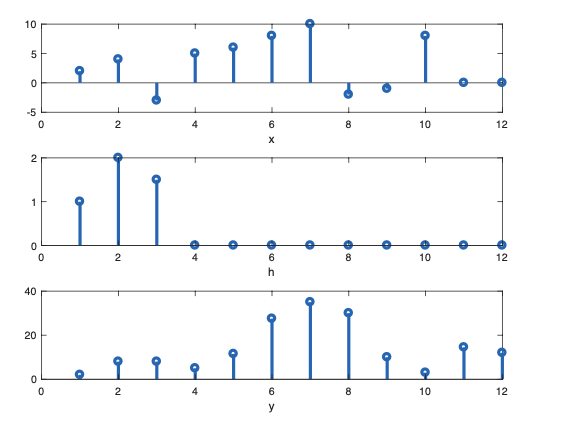
\includegraphics[width=0.5\linewidth]{img/linear_conv.png}
    \caption{A \(\in \mathbb{R}^{m \times n}\) with \(m = n + K - 1\) models the linear convolution.
}
    \label{fig:linear_conv}
\end{figure}


\begin{figure}[H]
    \centering
    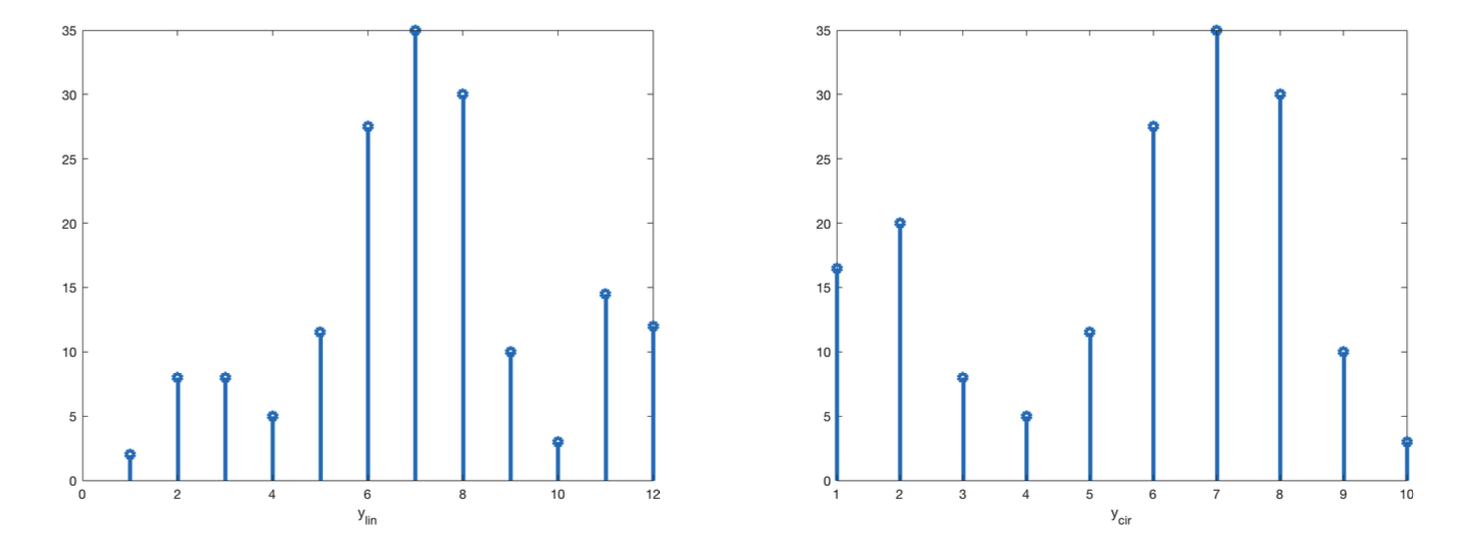
\includegraphics[width=1\linewidth]{img/cir_conv.png}
    \caption{If we want \(A\) to be square, we may assume that \(x \in \mathbb{R}^n\) is periodic outside the interval of observation. In this case \(A\) is a `circulant' matrix and models the circulant convolution.}
    \label{fig:circ-conv}
\end{figure}

\subsubsection*{Example of Linear and Circulant Convolution}
Assume you want to implement a discrete-time version of the derivative \( y(t) = \frac{dx(t)}{dt} \). The natural way to do it is by taking finite differences of the incoming sequence: \( y_n = x_n - x_{n-1} \). This is achieved by filtering with \( h_k = [1, -1] \):

\[
y_n = \sum_k h_k x_{n-k}
\]

In the case of linear convolution, the linear mapping is described by the \( (n + 1) \times n \) matrix:

\[
\mathbf{A} = \begin{bmatrix}
h_0&0&\cdots&0&0\\
h_1&h_0&&\vdots&\vdots\\
h_2&h_1&\cdots&0&0\\
\vdots&h_2&\cdots&h_0&0\\
h_{K-2}&\vdots&\ddots&h_1&h_0\\
h_{K-1}&h_{K-2}&&\vdots&h_1\\
0&h_{K-1}&\ddots&h_{K-3}&\vdots
\\0&0&\cdots&h_{K-2}&h_{K-3}\\
\vdots&\vdots&&h_{K-1}&h_{K-2}\\
0&0&0&\cdots&h_{K-1}\\
\end{bmatrix}=\begin{bmatrix}
1 & 0 & 0 & \cdots &0&0\\
-1& 1 & 0& \cdots &0&0\\
0 & -1& 1 & \cdots &0&0\\
\vdots&\vdots&\ddots& \ddots&\vdots&\vdots\\
0 & 0 & \cdots  & -1& 1 & 0\\
0 & 0 & \cdots  & 0 & -1 & 1 \\
0 & 0 & \cdots  & 0 &  0 & -1
\end{bmatrix}
\]

In the case of circulant convolution, the linear mapping is described by the \( n \times n \) matrix:

\[
\mathbf{A} = \begin{bmatrix}
1 & 0 & 0 & \cdots &0&0\\
-1& 1 & 0& \cdots &0&0\\
0 & -1& 1 & \cdots &0&0\\
\vdots&\vdots&\ddots& \ddots&\vdots&\vdots\\
0 & 0 & \cdots  & -1& 1 & 0\\
0 & 0 & \cdots  & 0 & -1 & 1 \\
\end{bmatrix}
\]




\subsection{Discrete-time Fourier Transform}

The discrete Fourier Transform (DFT) is a linear mapping and can be described by a matrix. Recall that given the finite-length sequence: $x_0, x_1, \cdots, x_{N-1}$ the DF is given by:

\[X_{r}=\sum_{n=0}^{N-1}x_{n}e^{-j2\pi\frac{rn}{N}}\quad r=0,1,...N-1\]

\[\begin{bmatrix}X_0\\X_1\\\vdots\\X_{N-1}\end{bmatrix}=\begin{bmatrix}1&1&1&\cdots&1\\1&e^{-j\frac{2\pi}N}&e^{-j\frac{4\pi}N}&\vdots&e^{-j2\pi\frac{N-1}N}\\1&e^{-j\frac{4\pi}N}&\vdots&\vdots&\vdots\\\vdots&\vdots&\vdots&\vdots&e^{-j2\pi\frac{(N-2)(N-2)}N}\\1&e^{-j2\pi\frac{N-1}N}&\cdots&e^{-j2\pi\frac{(N-1)(N-2)}N}&e^{-j2\pi\frac{(N-1)(N-1)}N}\end{bmatrix}\begin{bmatrix}x_0\\x_1\\\vdots\\\vdots\\x_{N-1}\end{bmatrix}\]





\section{Range and Null Space}

\subsection{Introduction}

Consider the linear transformation \( \mathbf{X} \rightarrow \mathbf{Y} \) represented by the matrix

\[ A = \begin{pmatrix}
1 & 2 & 0 \\
1 & 2 & 0 \\
0 & 0 & 1 \\
\end{pmatrix} \]

The matrix \( A \) maps vectors from \( \mathbb{R}^3 \) to \( \mathbb{R}^3 \). However, the first two rows of \( A \) are identical, indicating that all vectors \( \mathbf{X} \) are mapped to a plane in \( \mathbb{R}^3 \). This redundancy suggests that the mapping is not one-to-one since different vectors in \( \mathbb{R}^3 \) could result in the same vector in \( \mathbb{R}^3 \) after transformation. Consequently, we infer that the transformation is not invertible.\\

In an intuitive sense, the elements have been collapse into a 2D plane despite the mapping being from \( \mathbb{R}^3 \) to \( \mathbb{R}^3 \). Since information `is lost' after transformation, we feel that this mapping is not invertible.\\

The concepts of range space (or column space) and null space (or kernel) of \( A \) help to formalise this intuition. The range space is the set of all possible outputs \( \mathbf{Y} \), which, in this case, is a plane in \( \mathbb{R}^3 \). The null space is the set of all vectors \( \mathbf{X} \) that map to the zero vector in \( \mathbb{R}^3 \), indicating the loss of information and confirming the non-invertibility of the transformation.


\begin{figure}[H]
\begin{center}
\tdplotsetmaincoords{70}{110} % to set the orientation of the 3D plot
\begin{tikzpicture}[scale=1,tdplot_main_coords,>=stealth]

% Left R^3 axes
\draw[->] (0,0,0) -- (3,0,0) node[anchor=north east]{$y_1$};
\draw[->] (0,0,0) -- (0,3,0) node[anchor=north west]{$y_2$};
\draw[->] (0,0,0) -- (0,0,3) node[anchor=south]{$y_3$};

% Vectors in left R^3
\draw[->,thick,green] (0,0,0) -- (1,1,0);
\draw[->,thick,orange] (0,0,0) -- (2,2,0);
\draw[->,thick,purple] (0,0,0) -- (0,0,1);

% Plane 2x-y=0 (range space)
\fill[blue,opacity=0.3] (0,0,0) -- (3,3,0) -- (3,3,3) -- (0,0,3) -- cycle;
\node[anchor=south] at (3,4.2,0) {Range space};

% Right R^3 axes
\draw[->] (5,0,0) -- (8,0,0) node[anchor=north east]{$x_1$};
\draw[->] (5,0,0) -- (5,3,0) node[anchor=west]{$x_2$};
\draw[->] (5,0,0) -- (5,0,3) node[anchor=south]{$x_3$};

% Vectors in right R^3
\draw[->,thick,green] (5,0,0) -- (6,0,0);
\draw[->,thick,orange] (5,0,0) -- (5,1,0);
\draw[->,thick,purple] (5,0,0) -- (5,0,1);

% Connecting arrows
\draw[<->,dashed] (1,1,0) -- (6,0,0);
\draw[<->,dashed] (2,2,0) -- (5,1,0);
\draw[<->,dashed] (0,0,1) -- (5,0,1);

% Null space line
\draw[dotted, thick, red] (9,-2,0) -- (1,2,0);
\node[anchor=north] at (7,-2,0) {Null space};

\end{tikzpicture}
\end{center}
\caption{Visualised mapping}
\label{fig:mapping_linear_transform}

\end{figure}

We observe:
\begin{itemize}
    \item The columns of \textbf{A} are linearly dependent.
    \item The first and third column are only independent columns.
    \item The plane where all the vectors \textbf{x} were collapsing to is the $\text{span}\{ \begin{pmatrix}1\\1\\0\end{pmatrix},\begin{pmatrix}0\\0\\1\end{pmatrix}\}$, the range of the matrix
    \item We note that if $\mathbf{x} = \begin{pmatrix}
        2\\-1\\0
    \end{pmatrix}$ then $\mathbf{Ax} = 0$, so $\mathbf{x} = \begin{pmatrix}
        2\\-1\\0
    \end{pmatrix}$ is in the null space of \textbf{A} and is orthogonal to the range space.
\end{itemize}

\begin{definitionbox}{Range and Null Space}
Let \( A: X \rightarrow Y \) be a linear transformation. The \textbf{range space} \( \mathcal{R}(A) \) is the set of values in \( Y \) that are reached from \( X \) by applying \( A \):
\[ \mathcal{R}(A) = \{y = Ax : x \in X\} \]
The \textbf{null space} \( \mathcal{N}(A) \) is the set of values in \( X \) that are transformed to \( 0 \) by \( A \):
\[ \mathcal{N}(A) = \{x \in X : Ax = 0\} \]

Let \( A \) be an \( m \times n \) matrix which we regard as a linear operator and which we write as follows:
\[ A = [v_1 \quad v_2 \quad \ldots \quad v_n] \]
then a vector \( x \in \mathbb{R}^n \) is transformed as:
\[ Ax = x_1v_1 + x_2v_2 + \ldots + x_nv_n \]
which is a linear combination of the columns of \( A \).\\

This means that the range can be expressed as
\[ \mathcal{R}(A) = \text{span}\{v_1, v_2, \ldots, v_n\} \]
and corresponds to the column space of \( A \). Moreover, the number of linear independent columns of \( A \), which by definition is also the rank of \( A \), corresponds to the dimension of \( \mathcal{R}(A) \).\\

The null space of \( A \) is also a subspace and its dimension is \( n - \text{rank}(A) \).\\

When the dimension of \( \mathcal{N}(A) > 0 \) then the mapping is not invertible. Assume that \( An_1 = 0 \) and that \( y_1 = Ax_1 \), then, given \( x_2 = x_1 + n_1 \), we have that \( Ax_2 = Ax_1 + An_1 = Ax_1 = y_1 \). Therefore given \( y_1 \) it is not possible to know whether it is due to \( x_1 \) or \( x_2 \).\\

\textbf{Sketch of the Proof:}
\begin{itemize}
  \item Remember that when we compute \( Ax \) we are effectively taking a linear combination of the columns of \( A \)
  \item Assume for the sake of argument that \( \text{rank}(A) = n - 2 \), this means that given \( n - 2 \) columns of \( A \), the other two columns can be obtained with proper linear combinations of the linearly independent \( n - 2 \) columns.
  \item Therefore there are two linearly independent vectors \( x_1 \) and \( x_2 \) such that \( Ax_1 = Ax_2 = 0 \)
  \item Moreover any linear combination of \( x_1 \) and \( x_2 \) is also in the null space of \( A \), therefore that space has dimension 2.
\end{itemize}

Assume that \( A \) models a linear mapping from \( \mathbb{C}^n \) to \( \mathbb{C}^n \) and that its null space is non-trivial (i.e., it has dimension larger than 0 or \( \text{rank}(A) < n \)) then the mapping is not invertible or in other words the matrix \( A \) does not have an inverse.\\

In this case we call \( A \) a \textbf{singular matrix}.
    
\end{definitionbox}

\subsection{Computing the Nullspace}
\begin{itemize}
    \item Get row-echelon form (staircase) \textbf{u}
    \item Identify pivot columns and free columns
    \item To find nullspace solve $\textbf{ux} =0$
    \item Find the solution expressed as a function of free variables that correspond to the pivot columns position    
\end{itemize}

Let's consider matrix \( A \) and calculate its null space.

Given the matrix:
\[ A = \begin{bmatrix}
1 & 2 & 2 & 2 \\
2 & 4 & 6 & 8 \\
3 & 6 & 8 & 10
\end{bmatrix} \]

By applying elimination, we obtained the matrix \( u \):
\[ u = \left[ \begin{array}{cccc}
\color{red}1 & \color{red}2 & \color{blue}2 & \color{blue}2 \\
0 & 0 & \color{blue}2 & \color{blue}4 \\
0 & 0 & 0 & 0
\end{array} \right] \]

The matrix \( u \) contains two \textcolor{red}{pivot columns} shown in red and two \textcolor{blue}{free columns} shown in blue.

To calculate the null space \( \mathcal{N}(A) \), we need to solve the system \( Ax = 0 \). The system \( Ax = 0 \) is equivalent to \( ux = 0 \) which can be written as:
\[ ux = \begin{bmatrix}
\color{red}1 & \color{blue}2 & \color{red}2 & \color{blue}2 \\
0 & 0 & \color{red}2 & \color{blue}4 \\
0 & 0 & 0 & 0
\end{bmatrix}
\begin{bmatrix}
x_1 \\
x_2 \\
x_3 \\
x_4
\end{bmatrix} = 0 \]

Using row formulation, we obtain:
\begin{align*}
x_1 + 2x_2 + 2x_3 + 2x_4 &= 0 \\
2x_3 + 4x_4 &= 0 \\
\end{align*}

The solution of the above system is of the form:
\[
\begin{bmatrix}
x_1 \\
x_2 \\
x_3 \\
x_4
\end{bmatrix} = 
\begin{bmatrix}
-2x_2 + 2x_4 \\
x_2 \\
-2x_4 \\
x_4
\end{bmatrix} = x_2
\begin{bmatrix}
-2 \\
1 \\
0 \\
0
\end{bmatrix} + x_4
\begin{bmatrix}
2 \\
0 \\
-2 \\
1
\end{bmatrix}
\]

Variables \( x_2 \) and \( x_4 \) can take any values (free variables).\\

By assigning the value of 1 to a particular free variable and the value of 0 to the rest of the free variables, we obtain a so-called \textbf{special solution}.

The first special solution is obtained for \( x_2 = 1, x_4 = 0 \) and is:
\[
\begin{bmatrix}
-2 \\
1 \\
0 \\
0
\end{bmatrix}
\]

The second special solution is obtained for \( x_2 = 0, x_4 = 1 \) and is:
\[
\begin{bmatrix}
2 \\
0 \\
-2 \\
1
\end{bmatrix}
\]

The null space is the linear combination of the special solutions:
\[
\begin{bmatrix}
x_1 \\
x_2 \\
x_3 \\
x_4
\end{bmatrix} = c
\begin{bmatrix}
-2 \\
1 \\
0 \\
0
\end{bmatrix} + d
\begin{bmatrix}
2 \\
0 \\
-2 \\
1
\end{bmatrix}
\]

\section*{Range and Null Space for Linear Filtering}

\begin{itemize}
    \item Convolution and linear filtering are fundamental operations in signal processing. They can be algebraically represented using matrices.
    \item For linear systems, the convolution operation can be described by the Toeplitz matrix \( A \) through the equation \( y = Ax \), where \( y \) is the output signal and \( x \) is the input signal.
    \item The process of deconvolution aims to reverse this operation, attempting to retrieve the input signal \( x \) from the output signal \( y \).
    \item Understanding the range (or column space) and the null space of the matrix \( A \) is crucial because it informs us about the invertibility of the convolution operation. Specifically, the range tells us what outputs are possible, and the null space indicates if there are any inputs that could yield a zero output.
    \item \textbf{Claim} (without proof): If matrix \( A \) represents a linear convolution, then the null space is typically trivial, meaning there are no non-zero inputs that give a zero output. This is in contrast to circulant convolution, where the null space is generally non-trivial, allowing for the existence of non-zero inputs that do produce a zero output.
    \item \textbf{Example}: In the context of finite difference operations, consider a vector \( x \) consisting entirely of ones. For a circulant convolution matrix \( A \), this particular \( x \) would lie in the null space of \( A \), meaning that applying \( A \) to \( x \) would yield a zero vector, which signifies that no change would be detected in the signal.
\end{itemize}
\chapter{Matrix Theory Fundamentals}
\section{Determinant}

\noindent
The Determinant is a crucial number associated with square matrices, denoted either by $det(A)$ or $|A|$. A matrix $A$ is invertible iff (if and only if) $det(A) \neq 0$.

\noindent
Invertible matrix is called \textbf{non-singular.}
For a 2x2 matrix 
$
\begin{bmatrix}
a&b\\c&d
\end{bmatrix} $
the determinant is defined as 
$\begin{vmatrix}
a&b\\c&d
\end{vmatrix}$ $= ad-bc$.

\noindent

\begin{definitionbox}{Laplace's Formula for the Determinant} 
The determinant is defined as:

$det(\textbf{A}) = \sum^n_{j=1}(-1)^{i+j} a_{ij}M_{ij} $ for fixed i or \\
\noindent
$det(\textbf{A}) = \sum^n_{i=1}(-1)^{i+j} a_{ij}M_{ij} $ for fixed j 

This summation within can just be shortened to the produt of the cofactor and minor matrices within \textbf{A}, where:

\begin{itemize}
    \item The \emph{minor} \( M_{i,j} \) is defined to be the determinant of the \( (n - 1) \times (n - 1) \)-matrix that results from \( A \) by removing the \( i \)-th row and the \( j \)-th column.
    \item The \emph{cofactor} \( C_{i,j} \) is obtained by multiplying the minor by \( (-1)^{i+j} \).
\end{itemize}
\end{definitionbox}

\subsubsection*{Properties of Determinants}
\begin{enumerate}
    \item $det(I) = 1$ 
    \item Exchanging two rows of a matrix reverses the sign of the determinant. So an even number of exchanges keeps the determinant unchanged and an odd number of exchanges inverts the sign.
    \item Multiplying any row with a scalar multiplies the determinant by that scalar.
    \item Any row of zeroes leads to $det = 0$. \[
\begin{vmatrix}
0 & 0 \\
c & d
\end{vmatrix}
= 
\begin{vmatrix}
0 \cdot a & 0 \cdot b \\
c & d
\end{vmatrix}
=
0 \cdot
\begin{vmatrix}
a & b \\
c & d
\end{vmatrix}
= 0
\]
    \item Note that the determinant of the sum of two matrices is not necessarily the sum of their determinants:
\[
\begin{vmatrix}
a + a' & b + b' \\
c & d
\end{vmatrix} = \left(
\begin{vmatrix}
a  & b' \\
c & d
\end{vmatrix} + \begin{vmatrix}
a' & b' \\
c & d
\end{vmatrix} \right)
\neq
\begin{vmatrix}
a & b \\
c & d
\end{vmatrix}
+
\begin{vmatrix}
a' & b' \\
c & d
\end{vmatrix}
\]
In other words, \( \det(A + B) \neq \det(A) + \det(B) \). We observe `linearity' only for a single row
    \item Two equal rows leads to $det = 0$. This is inferred from the case of exchanging rows that changes the sign of the determinant – if we exchange two same rows, the final matrix is the same, so it should have the same sign – the only possible case of this is when $det=0$.
    \item Determinant after row reduction remains the same. \[
\begin{vmatrix}
a & b \\
c - la & d - lb
\end{vmatrix}
=
\begin{vmatrix}
a & b \\
c & d
\end{vmatrix}
+
\begin{vmatrix}
a & b \\
-la & -lb
\end{vmatrix}
=
\begin{vmatrix}
a & b \\
c & d
\end{vmatrix}
-
l
\begin{vmatrix}
a & b \\
a & b
\end{vmatrix}
=
\begin{vmatrix}
a & b \\
c & d
\end{vmatrix}
\]

\item Any upper or lower triangular matrix has the determinant that is the product of its diagonals.
\item Any singular matrix has $det = 0$ because eliminating the matrix gives it a row of zero. So this matrix is not full rank and is invertible. Any invertible matrix will have a non-zero determinant.
\item For square matrices $\textbf{A}$ and $\textbf{G}$ we have $det(\textbf{AB}) = det(\textbf{A})det(\textbf{B})$
    \item Moreover:
    \begin{itemize}
        \item The determinant of the inverse of \( A \) is the reciprocal of the determinant of \( A \):
        \[
        \det(A^{-1}) = \frac{1}{\det(A)}
        \]

        \item The determinant of \( A \) squared is the square of the determinant of \( A \):
        \[
        \det(A^2) = (\det(A))^2
        \]

        \item The determinant of a scalar multiple of \( A \) is the scalar raised to the \( n \)-th power times the determinant of \( A \), where \( A \) is an \( n \times n \) matrix and \( c \) is a scalar:
        \[
        \det(cA) = c^n\det(A)
        \]

    \end{itemize}

    \item The determinant of the transpose of \( A \) is equal to the determinant of \( A \):
    \[
    \det(A^T) = \det(A).
    \]
\end{enumerate}



\section{Rank and Trace}

\begin{definitionbox}{Rank of a matrix}
Given an \( m \times n \) matrix \( A \), the rank of \( A \), denoted \( \text{rank}(A) \), is the number of linearly independent rows or columns; in particular, if \( m = n \), \( \text{rank}(A) = n \) if and only if \( \det(A) \neq 0 \).

Properties (without proof):
\begin{itemize}
    \item For a rectangular matrix \( \text{rank}(A) \leq \min(n, m) \).
    \item \( \text{rank}(AB) \leq \min(\text{rank}(A), \text{rank}(B)) \).
\end{itemize}
\end{definitionbox}

\begin{definitionbox}{Trace of a matrix}
The trace of an \( n \times n \) matrix is defined as the sum of the elements along the main diagonal. Moreover:
\begin{itemize}
    \item \( \text{trace}(ABC) = \text{trace}(BCA) = \text{trace}(CAB) \).
    \item (Frobenius norm): \( \|A\|_F = \sqrt{\sum_{i,j} |a_{i,j}|^2} = \sqrt{\text{trace}(A^HA)} \) where \( A^H \) denotes the conjugate transpose of \( A \).
\end{itemize}
\end{definitionbox}


\section{Eigenvectors and Eigenvalues}
Consider a matrix \( A \) and a vector \( x \). The operation \( Ax \) produces a vector \( y \) at some direction. We are interested in vectors \( y \) which lie in the same direction as \( x \).\\    

In that case we have \( \textbf{Ax} = \lambda I \textbf{x} \) with \( \lambda \) being a scalar. Because the LHS is matrix multiplication and the RHS is scalar multiplication, we generally add in the identity matrix $I$ to help distinguish this:

\begin{align*}
    \textbf{Ax} &= \lambda I\textbf{x}\\
    (\textbf{A}-\lambda I)\textbf{x} &= 0
\end{align*}

 When the above relationship holds, \( x \) is called an \textit{eigenvector} and \( \lambda \) is called an \textit{eigenvalue} of matrix \( A \).\\

To solve this, if we know $(\textbf{A}-\lambda I)\textbf{x} = 0$, then $det((\textbf{A}-\lambda I)\textbf{x}) = 0$

If \( A \) is singular then \( \lambda = 0 \) is an eigenvalue.\\

Why are we interested in the eigenvectors and eigenvalues of a matrix? Because they make the solution of complex problems simpler. For example, if we know the eigenvectors and eigenvalues of a linear mapping \( y = Ax \) we can characterize that mapping easily.\\ If \( A = \begin{bmatrix} 3 & 1 \\ 1 & 3 \end{bmatrix} \), eigenvalues: \( \lambda_1 = 4 \), \( \lambda_2 = 2 \), eigenvectors: \( u_1 = \begin{bmatrix} 1 \\ 1 \end{bmatrix} \), \( u_2 = \begin{bmatrix} -1 \\ 1 \end{bmatrix} \).
Then \( x = a_1u_1 + a_2u_2 \) implies \( y = \lambda_1a_1u_1 + \lambda_2a_2u_2 \).

\begin{figure}[H]
    \centering
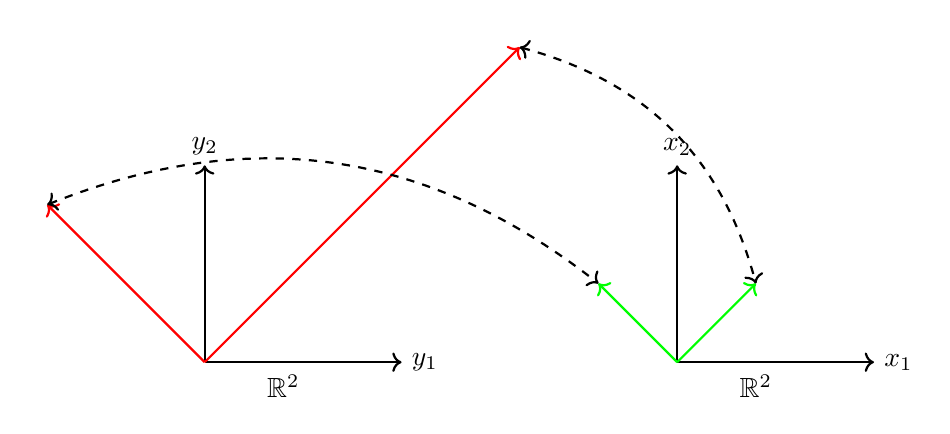
\begin{tikzpicture}[scale=1]

% Left plot (R^2 with y1, y2)
\begin{scope}[shift={(-3,0)}]
    % Axes
    \draw[thick,->] (0,0) -- (2.5,0) node[right] {$y_1$};
    \draw[thick,->] (0,0) -- (0,2.5) node[above] {$y_2$};
    % Vectors
    \draw[->, thick, red] (0,0) -- (4,4) node[above right] {};
    \draw[->, thick, red] (0,0) -- (-2,2) node[above left] {};
    % Label
    \node at (1,-0.3) {$\mathbb{R}^2$};
\end{scope}

% Right plot (R^2 with x1, x2)
\begin{scope}[shift={(3,0)}]
    % Axes
    \draw[thick,->] (0,0) -- (2.5,0) node[right] {$x_1$};
    \draw[thick,->] (0,0) -- (0,2.5) node[above] {$x_2$};
    % Vectors
    \draw[->, thick, green] (0,0) -- (1,1) node[above right] {};
    \draw[->, thick, green] (0,0) -- (-1,1) node[above left] {};
    % Label
    \node at (1,-0.3) {$\mathbb{R}^2$};
\end{scope}

% Curved double-ended arrows connecting corresponding vectors
% Connecting (4,4) in the left plot with (1,1) in the right plot
\draw[<->, thick, dashed] (-3+4,4) to[bend left] (3+1,1);
% Connecting (-2,2) in the left plot with (-1,1) in the right plot
\draw[<->, thick, dashed] (-3-2,2) to[bend left] (3-1,1);

\end{tikzpicture}

    \caption{Characterised mapping}
    \label{fig:eigens}
\end{figure}

In electrical engineering, we have already seen a few examples of this, for example, in continuous-time, such as the Signals and Systems module on eigen-functions of an LTI system leading to the convolution formula in the Fourier domain, and the solutions of linear differential equations in Control Systems.\\

In the discrete-time finite dimensional case, eigenvalues and eigenvectors are very important for discrete-time convolution and for difference equations.\\

\subsection{Eigenvectors and Eigenvalues of a permutation matrix}

Consider permutation matrix $\textbf{A} = \begin{bmatrix}
    0 & 1 \\ 1 & 0
\end{bmatrix}$.

It will have eigenvector $\begin{bmatrix}
    1\\1
\end{bmatrix}$ with corresponding eigenvalue $\lambda = 1$, and eigenvector $\begin{bmatrix}
    -1\\1
\end{bmatrix}$ with corresponding eigenvalue $\lambda = -1$.

Note that $n\times n$ matrices will have $n$ eigenvalues, but it is not easy to find them. In this syllabus, we do not go into much detail about the properties of eigenvalues and eigenvectors of a permutation matrix, but we can say that since permutation matrices are orthogonal, the eigenvectors span an orthogonal basis.\\

\subsubsection*{Properties}
\begin{itemize}
    \item The sum of eigenvalues, the \textbf{trace} of the matrix, equals the sum of the diagonal elements of the matrix.
    \item The product of eigenvalues equals the determinant of the matrix.
    \item We could have worked out the second eigenvalue of \textbf{A} by simply dividing the determinant by the first eigenvalue
\end{itemize}

\subsection{Solving for Eigenvalues and Eigenvectors}
\begin{definitionbox}{Finding Eigenvalues}
The eigenvalues of a matrix $A$ are found by solving the characteristic equation:
\[
\det(A - \lambda I) = 0
\]
where $I$ is the identity matrix of the same size as $A$.
\end{definitionbox}

\begin{definitionbox}{Finding Eigenvectors}
Once the eigenvalues $\lambda_i$ are found, the corresponding eigenvectors $v_i$ are found by solving the system of linear equations given by:
\[
(A - \lambda_i I)v_i = 0
\]
This system is solved for each eigenvalue $\lambda_i$. Note that there exists families of eigenvectors, not single eigenvectors.
\end{definitionbox}

\subsubsection*{Example}
For matrix $A = \begin{pmatrix}
2 & 1 \\
1 & 2
\end{pmatrix}$, we find eigenvalues by solving $\det(A - \lambda I) = 0$:

\[
\begin{vmatrix}
2 - \lambda & 1 \\
1 & 2 - \lambda
\end{vmatrix} = (2-\lambda)^2 - 1 = \lambda^2 - 4\lambda + 3 = 0
\]

This gives $\lambda_1 = 1$ and $\lambda_2 = 3$. The eigenvectors are found by substituting $\lambda_i$ back into $(A - \lambda_i I)v_i = 0$.

\subsubsection*{Example}
Consider the matrix 
\[ A = \begin{bmatrix}
3 & 1 \\
0 & 3
\end{bmatrix}. \]

The sum of the eigenvalues \( \lambda_1 + \lambda_2 \) is equal to the trace of \( A \), which is 6, and the product \( \lambda_1 \lambda_2 \) is equal to the determinant of \( A \), which is 9.

To find the eigenvalues, we calculate the determinant of \( A - \lambda I \):
\[ \det(A - \lambda I) = \det \begin{bmatrix}
3 - \lambda & 1 \\
0 & 3 - \lambda
\end{bmatrix} = (3 - \lambda)^2 = 0 \Rightarrow \lambda_{1,2} = 3. \]

\textbf{The eigenvalues of a triangular matrix are the values of the diagonal.}

For this particular case, we have:
\[ \begin{bmatrix}
3 & 1 \\
0 & 3
\end{bmatrix}
\begin{bmatrix}
x \\
y
\end{bmatrix}
=
\begin{bmatrix}
3x \\
3y
\end{bmatrix}
\Rightarrow y = 0 \text{ and } x \text{ can be any number.}
\]
\subsection{Special Case: Eigenvalues with Identity Matrix Addition}
Consider the matrix $\textbf{A} = \textbf{B} + c\textbf{I}$.\\

Consider an eigenvector \textbf{x} and eigenvalue $\lambda$ of \textbf{B}.\\

Then \textbf{Bx} = $\lambda\textbf{x}$ and so:\\

\begin{align*}
    \textbf{Ax} &= (\textbf{B} + c\textbf{I})\textbf{x}\\
    &= \textbf{Bx} + c\textbf{Ix}\\
    &= \textbf{Bx} + c\textbf{x}\\
    &= \lambda\textbf{x} + c\textbf{x}\\
    &= (\lambda+ c)\textbf{x}
\end{align*}

From this we can say \textbf{A} has the same eigenvectors as \textbf{B} with eigenvalues $\lambda + c$.
% \subsubsection*{Properties}


\section{Diagonalisation of Matrices}
\begin{itemize}
    \item Suppose we have \( n \) linearly independent eigenvectors of a matrix \( A \), denoted by \( \mathbf{x}_i \).
    \item The corresponding eigenvalues are \( \lambda_i \).
    \item These eigenvectors are arranged as columns in a matrix \( S \), forming the so-called eigenvector matrix.
    \item By forming the product \( AS \), where \( S = [\mathbf{x}_1 \mathbf{x}_2 \ldots \mathbf{x}_n] \), we effectively scale each eigenvector by its corresponding eigenvalue:
    \[
    AS = A[\mathbf{x}_1 \mathbf{x}_2 \ldots \mathbf{x}_n] = [\lambda_1\mathbf{x}_1 \lambda_2\mathbf{x}_2 \ldots \lambda_n\mathbf{x}_n] = S\Lambda
    \]
    where \( \Lambda \) is a diagonal matrix with eigenvalues \( \lambda_i \) on its diagonal and zeros elsewhere:
    \[
    \Lambda = \begin{bmatrix}
    \lambda_1 & 0 & \ldots & 0 \\
    0 & \lambda_2 & \ldots & 0 \\
    \vdots & \vdots & \ddots & \vdots \\
    0 & 0 & \ldots & \lambda_n
    \end{bmatrix}
    \]
    \item This gives us the fundamental relationship \( AS = S\Lambda \), which implies \( A = S\Lambda S^{-1} \) when \( S \) is invertible.
    \item The process of transforming \( A \) into \( \Lambda \) through the similarity transformation \( S \) is called \emph{matrix diagonalisation}.
    \item Matrix diagonalisation is particularly important in Mathematics and Engineering because it simplifies many matrix computations and provides a clear framework for understanding linear transformations.
\end{itemize}

\subsection{Matrix Diagonalisation and Commutativity}

\textbf{Theorem:} Matrices \( A \) and \( B \) are simultaneously diagonalisable, sharing the same eigenvector matrix \( S \), if and only if \( AB = BA \).\\

\textit{Sketch of the proof:} Given that \( A \) and \( B \) are diagonalisable, we can write \( A = S\Lambda_1S^{-1} \) and \( B = S\Lambda_2S^{-1} \). Thus, 
\[ AB = S\Lambda_1S^{-1}S\Lambda_2S^{-1} \] 
and 
\[ BA = S\Lambda_2S^{-1}S\Lambda_1S^{-1} \].
Since \( \Lambda_1\Lambda_2 = \Lambda_2\Lambda_1 \) (as they are diagonal matrices), it follows that \( AB = BA \).\\

A matrix has \( n \) independent eigenvectors and therefore is diagonalisable if all the eigenvalues are different.\\

If \( Ax = \lambda x \) then \( A^2x = A(Ax) = A(\lambda x) = \lambda (Ax) = \lambda^2 x \). Therefore, the eigenvalues of \( A^2 \) are \( \lambda^2 \). The eigenvectors of \( A^2 \) remain the same since \( A^2 = SAS^{-1}SAS^{-1} = S\Lambda^2S^{-1} \). In general, for any positive integer \( k \), \( A^k = S\Lambda^kS^{-1} \).\\

If there are repeated eigenvalues a matrix may, or may not have independent eigenvectors. For example, consider the identity matrix. Its eigenvectors are the row (or column) vectors. They are all independent, but the eigenvalues are all equal to 1.\\
 \begin{examplebox}{A and B sharing Eigenvectors}
\subsubsection*{Question}
If \( A \) and \( B \) share the same eigenvectors, what can we say about the eigenvalues of \( AB \)?

\subsubsection*{Answer} Since $A$ and $B$ share the same eigenvectors, $AB$ will also have the same eigenvectors. Let $v$ be an eigenvector of $A$ and $B$, then $Av = \lambda v$ and $Bv = \mu v$ for some eigenvalues $\lambda$ and $\mu$ of $A$ and $B$ respectively. Thus:

\[ABv = A(\mu v) = \mu Av = \mu\lambda v\]

Showing us that $v$ is also an eigenvector of $AB$ with corresponding eigenvalue $\mu\lambda$. But this does not tell us that all eigenvalues of $AB$ are necessarily products of eigenvalues of $A$ and $B$. $A$ and $B$ must be diagonalisable and $A,B$ are commutative so $AB = BA$. $A=PDP^{-1}$ and $B = PQP^{-1}$, where $D$ and $Q$ are diagonal matrices with eigenvalues of $A$ and $B$ respectively, and $P$ is the matrix of shared eigenvectors. Then $AB = PDQP^{-1}$, and the eigenvectors form a basis, so diagonal entries of $DQ$ will be eigenvalues of $AB$ since the determinant between the two are preserved. \\
\end{examplebox}

\begin{examplebox}{Inverting a Diagonalisable Square Matrix}    

\subsubsection*{Question} If \( A = S\Lambda S^{-1} \) is square and invertible, can you compute \( A^{-1} \)?

\subsubsection*{Answer} If \( A \) is invertible, then \( A^{-1} = S\Lambda^{-1}S^{-1} \), where \( \Lambda^{-1} \) is the diagonal matrix with the reciprocal of \( A \)'s eigenvalues on the diagonal.
\end{examplebox}


\section{Difference Equations}
\subsection*{Fibonacci Sequence Analysis}

The Fibonacci sequence (0,1,1,2,3,5,8,13...) is a series of numbers where each number is the sum of the two preceding ones, typically starting with 0 and 1. Mathematically, it can be expressed as:
\begin{equation}
    F_{k+2} = F_{k+1} + F_k
\end{equation}
where $F_k$ represents the $k$-th term of the Fibonacci sequence.

To solve this using linear algebra, we can define the state vector $u_k$:
\begin{equation}
    u_k = \begin{bmatrix}
    F_{k+1} \\
    F_k
    \end{bmatrix}
\end{equation}
By employing the recursive definition of the Fibonacci sequence, we obtain the matrix form:
\begin{equation}
    u_{k+1} = A u_k = \begin{bmatrix}
    1 & 1 \\
    1 & 0
    \end{bmatrix} u_k
\end{equation}
Given the initial state vector $u_0$ that we know of, the state at any point $k$ is given by:
\begin{equation}
    u_k = A^k u_0
\end{equation}
If $A$ can be diagonalized as $A = S \Lambda S^{-1}$, where $\Lambda$ is a diagonal matrix of eigenvalues and $S$ is a matrix of corresponding eigenvectors, then the computation simplifies to:
\begin{equation}
    u_k = S \Lambda^k S^{-1} u_0
\end{equation}
Thus, knowing the eigenvectors and eigenvalues of $A$ can greatly simplify the computation of terms in the Fibonacci sequence.

\subsection*{System of Difference Equations}

Consider a system described by a set of difference equations:
\begin{align}
    y_1[n+1] &= y_1[n] - 1.5y_2[n] \\
    y_2[n+1] &= 0.5y_1[n] + y_2[n]
\end{align}
This system can be written in matrix form using the state vector $u_n$:
\begin{equation}
    u_n = \begin{bmatrix}
    y_1[n] \\
    y_2[n]
    \end{bmatrix}
\end{equation}
Thus, the next state $u_{n+1}$ is given by:
\begin{equation}
    u_{n+1} = A u_n = \begin{bmatrix}
    1 & -1.5 \\
    0.5 & 1
    \end{bmatrix} u_n
\end{equation}
Given $u_0$, the state $u_n$ is then:
\begin{equation}
    u_n = A^n u_0
\end{equation}
As with the Fibonacci sequence, if $A$ can be diagonalized, the solution becomes more tractable:
\begin{equation}
    u_n = S \Lambda^n S^{-1} u_0
\end{equation}
Hence, eigenvalues and eigenvectors are key to simplifying the solution of the system of difference equations, providing a powerful method to analyze and solve linear discrete-time systems in signals and systems.\\

\section{Markov Processes}
Markov processes are used to model systems that undergo transitions from one state to another on a state space. A key feature of a Markov process is that the future state depends only on the current state and not on the sequence of events that preceded it.\\


Consider a Markov process example inspired by Strang's book, modelling population migration between California and the outside:
\begin{quote}
    ``Assume that each year 1/10 of the people outside California move in and 2/10 of the people inside California move out."
\end{quote}

Let $y_0$ be the initial population outside California and $z_0$ the initial population inside California. The state vector and the transition matrix $A$ are given by:
\begin{equation}
    \begin{bmatrix}
    y_1 \\
    z_1 
    \end{bmatrix} = 
    \begin{bmatrix}
    0.9 & 0.2 \\
    0.1 & 0.8 
    \end{bmatrix}
    \begin{bmatrix}
    y_0 \\
    z_0 
    \end{bmatrix} = A 
    \begin{bmatrix}
    y_0 \\
    z_0 
    \end{bmatrix}
\end{equation}


The eigenvalues and eigenvectors of $A$ are crucial for understanding the long-term behavior of the Markov process. In this case, the eigenvalues are $\lambda_1 = 1$ and $\lambda_2 = 0.7$, with corresponding eigenvectors:
\begin{equation}
    \mu_1 = \begin{bmatrix}
    2/3 \\
    1/3 
    \end{bmatrix}, \quad
    \mu_2 = \begin{bmatrix}
    1 \\
    -1 
    \end{bmatrix}
\end{equation}
We can then write the state at instant $k$ as:
\begin{equation}
    \begin{bmatrix}
    y_k \\
    z_k 
    \end{bmatrix} = A^k
    \begin{bmatrix}
    y_0 \\
    z_0 
    \end{bmatrix}
\end{equation}

For a large $k$, the contribution from the second eigenvalue becomes negligible, leading to a steady-state solution where the population distribution does not change from one year to the next:
\begin{equation}
    \begin{bmatrix}
    y_{\infty} \\
    z_{\infty} 
    \end{bmatrix} = \left( y_0 + z_0 \right)
    \begin{bmatrix}
    2/3 \\
    1/3 
    \end{bmatrix}
\end{equation}

\subsection*{Properties of Transition Matrices}

From this example, we can deduce some general properties of Markov or transition matrices:
\begin{itemize}
    \item All entries are non-negative.
    \item Each column of the matrix adds up to one, ensuring the total probability is conserved.
    \item The eigenvalue $\lambda_1 = 1$ corresponds to the steady state.
    \item All other eigenvalues $\lambda_i$ satisfy $|\lambda_i| \leq 1$.
\end{itemize}
Additionally, it can be shown that $\lambda_1 = 1$ is always an eigenvalue by noting that each column of $A - I$ sums to zero, indicating that $A - I$ is singular and thus $\lambda_1 = 1$ is an eigenvalue. The corresponding eigenvector represents the steady-state distribution since $A\mu_1 = \mu_1$. This implies that in the long run, the system will reach a state where the population distribution remains constant if no external changes are made to the system.

\subsection*{Computing the State at Instant \( k \)}

Given the eigendecomposition of \( A \) as \( A = S \Lambda S^{-1} \), where \( S \) is the matrix of eigenvectors and \( \Lambda \) is the diagonal matrix of eigenvalues, the state at any instant \( k \) can be computed as:
\begin{equation}
    \begin{bmatrix}
    y_k \\
    z_k 
    \end{bmatrix} = S \Lambda^k S^{-1}
    \begin{bmatrix}
    y_0 \\
    z_0 
    \end{bmatrix}
\end{equation}

For our specific matrix \( A \), the computation yields:
\begin{equation}
    \begin{bmatrix}
    y_k \\
    z_k 
    \end{bmatrix} = 
    \begin{bmatrix}
    2/3 & 1/3 \\
    1/3 & -1/3 
    \end{bmatrix}
    \begin{bmatrix}
    1 & 0 \\
    0 & (0.7)^k 
    \end{bmatrix}
    \begin{bmatrix}
    1 & 1 \\
    1 & -2 
    \end{bmatrix}
    \begin{bmatrix}
    y_0 \\
    z_0 
    \end{bmatrix}
\end{equation}

\subsection*{Steady-State Solution}

The steady-state solution, which occurs as \( k \) approaches infinity, is given by the eigenvector corresponding to \( \lambda_1 = 1 \):
\begin{equation}
    \begin{bmatrix}
    y_{\infty} \\
    z_{\infty} 
    \end{bmatrix} = 
    \left( y_0 + z_0 \right)
    \begin{bmatrix}
    2/3 \\
    1/3 
    \end{bmatrix}
\end{equation}
This indicates that regardless of the initial state, the system will evolve into a state where the ratios of the populations inside and outside California are \( 2:1 \), respectively.

\subsection*{General Observations}

The model demonstrates a fundamental principle of Markov processes: despite potentially complex dynamics, the long-term behaviour is determined by the eigenvalues and eigenvectors of the transition matrix, with the largest eigenvalue indicating the steady state. This simplifies the analysis of systems described by Markov processes, particularly in the fields of signals and systems, stochastic processes, and population dynamics.



\section{Diagonalisation of Circulant Matrices}

Diagonalization of circulant matrices is closely tied to the concept of convolution in signal processing. A circulant matrix \( A \) can model the circular convolution operation between an input vector \( \mathbf{x} \) and a filter \( \mathbf{h} \), resulting in an output vector \( \mathbf{y} \) such that \( \mathbf{y} = A\mathbf{x} \).

\subsubsection*{Discrete Fourier Transform (DFT)}

The Discrete Fourier Transform (DFT) plays a pivotal role in the analysis of circulant matrices. For a DFT matrix of size \( n \times n \), the element in the \( i \)-th row and \( k \)-th column is given by \( w_n^{ik} \), where \( w_n = e^{-j\frac{2\pi}{n}} \). The DFT matrix \( W \) has the following form:

\[
W = \frac{1}{\sqrt{n}} \begin{bmatrix} 
1 & 1 & 1 & \cdots & 1 \\
1 & w_n & w_n^2 & \cdots & w_n^{n-1} \\
1 & w_n^2 & w_n^4 & \cdots & w_n^{2(n-1)} \\
\vdots & \vdots & \vdots & \ddots & \vdots \\
1 & w_n^{n-1} & w_n^{2(n-1)} & \cdots & w_n^{(n-1)(n-1)}
\end{bmatrix}
\]

\subsubsection*{Eigenvectors and Eigenvalues}

The eigenvectors of a circulant matrix are precisely the columns of the DFT matrix \( W \). These eigenvectors, denoted as \( \mathbf{u}_i \), can be expressed as:

\[
\mathbf{u}_i = \frac{1}{\sqrt{n}} \begin{bmatrix}
1 \\
w_n^i \\
w_n^{2i} \\
\vdots \\
w_n^{(n-1)i}
\end{bmatrix}
\]

The eigenvalues of a circulant matrix are the DFT of the first row of the matrix, which corresponds to the filter \( \mathbf{h} \). This direct correspondence facilitates the use of DFT in signal processing to perform efficient convolution operations.

\subsubsection*{Diagonalization by DFT}

The DFT matrix \( W \) has the property of diagonalizing a circulant matrix \( A \). This means that \( A \) can be represented as \( A = W \Lambda W^{-1} \), where \( \Lambda \) is a diagonal matrix containing the eigenvalues of \( A \). As a result, the DFT simplifies the multiplication of a circulant matrix with a vector, transforming it into a multiplication of the diagonal matrix \( \Lambda \) with the DFT of the vector.

\subsubsection*{Implications in Signal Processing}

In signal processing, this diagonalization property is exploited for efficient computation of convolutions, particularly using algorithms such as the Fast Fourier Transform (FFT), which is a computationally efficient implementation of the DFT. Thus, the DFT forms the basis for many signal processing techniques, enabling the analysis and manipulation of signals in the frequency domain.

\section{Complex, Symmetric, Hermitian Matrices}

Symmetric matrices are a fundamental concept in linear algebra with important implications in various fields, including signal processing and systems theory. 

\subsection*{Definition and Properties}

\begin{itemize}
    \item A real matrix \( A \) is said to be symmetric if \( A = A^T \), where \( A^T \) denotes the transpose of \( A \).
    \item For complex matrices, symmetry is defined by the condition \( A^* = A \), where \( A^* \) denotes the conjugate transpose of \( A \). Such matrices are also known as \textit{Hermitian matrices}.
    \item The notation \( A^H \) is also commonly used to denote the conjugate transpose, so for Hermitian matrices, \( A^H = A \).
    \item Symmetric matrices are prevalent in numerous applications, notably in statistics as covariance matrices.
    \item It is an established fact that the eigenvalues of a symmetric matrix are real numbers. This will be demonstrated through a proof.
    \item Additionally, eigenvectors of a symmetric matrix corresponding to distinct eigenvalues are orthogonal. The proof of this statement is provided in a subsequent section.
    \item For symmetric matrices with orthonormal eigenvectors, we can represent \( A \) as \( A = Q\Lambda Q^T \), where \( Q \) is the matrix of eigenvectors, and \( \Lambda \) is the diagonal matrix of eigenvalues.
\end{itemize}

\subsection*{Eigenvalues and Eigenvectors}
\begin{examplebox}{Proof of Complex Conjugate Pairs for Eigenvalues}
\subsubsection*{Question}

Prove that the eigenvalues of a symmetric matrix occur in complex conjugate pairs.

\subsubsection*{Solution}

Consider the eigenvalue equation \( Ax = \lambda x \).

\begin{itemize}
    \item Taking the complex conjugate of both sides of the equation yields \( (Ax)^* = (\lambda x)^* \) which simplifies to \( A^* x^* = \lambda^* x^* \).
    \item If \( A \) is a real symmetric matrix, then \( A^* = A \), and hence \( \lambda^* x^* \) must also be an eigenvector-eigenvalue pair, i.e., if \( \lambda \) is an eigenvalue of \( A \) with corresponding eigenvector \( x \), then \( \lambda^* \) is also an eigenvalue of \( A \) with corresponding eigenvector \( x^* \).
\end{itemize}

\end{examplebox}

\begin{examplebox}{Proof that Symmetric Matrices' Eigenvalues are Real}
\subsubsection*{Question}
Prove that the eigenvalues of a symmetric matrix are real.

\subsubsection*{Solution}

We have previously shown that for a real matrix \( A \), the complex conjugate of an eigenvalue \( \lambda \) is also an eigenvalue. Let's consider the eigenvalue equation \( Ax = \lambda x \).

\begin{enumerate}
    \item Taking the transpose of both sides of the equation yields \( x^T A^T = \lambda x^T \). Since \( A \) is symmetric, \( A^T = A \), so this becomes \( x^T A = \lambda x^T \).
    \item Multiplying both sides from the right by \( x \), we get \( x^T Ax = \lambda x^T x \).
    \item Now, we take the eigenvalue equation \( Ax = \lambda x \) and multiply both sides from the left with \( x^T \) to obtain \( x^T Ax = \lambda x^T x \).
    \item Observing the above, since \( x^T x \) is a scalar and \( x^T x \neq 0 \), it implies that \( \lambda \) must be equal to its complex conjugate \( \lambda^* \), which means \( \lambda \) is real.
\end{enumerate}
  
\end{examplebox}
\begin{examplebox}{Proof that Eigenvectors of a Symmetric Matrix with Unique Eigenvalues are always Orthogonal}
\subsubsection*{Question}
Prove that the eigenvectors of a symmetric matrix corresponding to different eigenvalues are always orthogonal.

\subsubsection*{Solution}

Let \( Ax = \lambda_1 x \) and \( Ay = \lambda_2 y \) be two eigenvectors of \( A \) corresponding to distinct eigenvalues \( \lambda_1 \neq \lambda_2 \).

\begin{enumerate}
    \item Taking the dot product of \( Ax \) with \( y \) yields \( (Ax)^T y = \lambda_1 x^T y \).
    \item Since \( A \) is symmetric, \( (Ax)^T y = x^T A^T y = x^T Ay = x^T \lambda_2 y \).
    \item These conditions imply \( \lambda_1 x^T y = \lambda_2 x^T y \) and since \( \lambda_1 \neq \lambda_2 \), it follows that \( x^T y = 0 \).
    \item Thus, the eigenvectors \( x \) and \( y \) are orthogonal.
\end{enumerate}



\end{examplebox}




\begin{definitionbox}{A Hermitian Matrix always has Real Eigenvectors}
\begin{itemize}
    \item We aim to determine which complex matrices have real eigenvalues and orthogonal eigenvectors.
    \item Consider the eigenvalue equation \( Ax = \lambda x \) with \( A \) possibly complex.
    \item Taking the complex conjugate on both sides yields \( (Ax)^* = (\lambda x)^* \) which implies \( A^* x^* = \lambda^* x^* \).
    \item By transposing both sides, we obtain \( x^{*T} A^{*T} = \lambda^* x^T \).
    \item Multiplying both sides from the right by \( x \), we get \( x^* A^* x = \lambda^* x^T x \).
    \item Starting again with \( Ax = \lambda x \) and multiplying both sides from the left by \( x^* \), we have \( x^* Ax = \lambda x^* x \).
\end{itemize}
    From the above steps, we deduce that if \( A^{*T} = A \), then \( \lambda x^* x = \lambda^* x^* x \) and since \( x^* x \neq 0 \), it follows that \( \lambda = \lambda^* \).
\end{definitionbox}

\begin{examplebox}{Proof of Orthogonal Eigenvectors for unique Eigenvectors in Hermitian Matrices\\ }
\subsubsection*{Question:}
Prove that the eigenvectors of a complex symmetric matrix (Hermitian matrix) which correspond to different eigenvalues are always perpendicular.

\subsubsection*{Solution:}
Suppose $Ax = \lambda_1 x$ and $Ay = \lambda_2 y$,where $\lambda_1 \neq \lambda_2$. We have

\[(\lambda_1x)^Hy=x^H\lambda_1y=(Ax)^Hy=x^HAy=x^H\lambda_2y\]

The conditions $x^H \lambda_1 y = x^H \lambda_2 y$ and $\lambda_1 \neq \lambda_2$, give $x^H$ = 0, so these eigenvalues $x$ and $y$ are perpendicular.
\end{examplebox}

\subsection{Spectral Theorem}

We have demonstrated that:
\begin{itemize}
    \item The eigenvalues of a symmetric matrix, whether real or complex, are real.
    \item The eigenvectors of a symmetric matrix, whether real or complex, that correspond to different eigenvalues are orthogonal.
\end{itemize}

We conclude this part with the following statement (without proof):
\begin{itemize}
    \item \textbf{Spectral theorem}: Every real symmetric matrix can be diagonalised by an orthogonal matrix, and every Hermitian matrix can be diagonalised by a unitary matrix:
    \begin{itemize}
        \item For the real case: \( A = Q \Lambda Q^{-1} = Q \Lambda Q^T \)
        \item For the complex case: \( A = Q \Lambda Q^{-1} = Q \Lambda Q^H \)
    \end{itemize}
\end{itemize}

\subsection{Positive Definite Hermitian Matrices}



\begin{definitionbox}{Positive Definite Hermitian Matrices}
    Hermitian matrix \textbf{A} is positive definite if and only if:

    \begin{itemize}
        \item $\textbf{x}^H\textbf{Ax} > 0$ and $\textbf{x} \neq 0$
        \item All eigenvalues of \textbf{A} satisfy $\lambda_i > 0$
        \item All pivots without row exchanges satisfy $ d_i>0$
    \end{itemize}
\end{definitionbox}

\begin{examplebox}{Positive Definite Test for Identifying Stationary Points}
Consider the function \( f(x_1, x_2) = a_{11}x_1^2 + 2a_{12}x_1x_2 + a_{22}x_2^2 \).

\begin{itemize}
    \item It is evident that \( f(0,0) = 0 \) and at the point \( (0,0) \), we also have \(\frac{\partial f}{\partial x_1} = \frac{\partial f}{\partial x_2} = 0\).
    \item The question is: Is \( (0,0) \) a minimum, a maximum, or a saddle point?
    \item If the matrix \( A \) defined as
    \[
    A =
    \begin{bmatrix}
    a_{11} & a_{12} \\
    a_{12} & a_{22}
    \end{bmatrix}
    \]
    is positive definite, then \( (0,0) \) is a minimum. If \( A \) is negative definite, then it is a maximum. If \( A \) is indefinite, then \( (0,0) \) is a saddle point.
\end{itemize}

In general, for a function in several variables of the form \( f(\mathbf{x}) = \sum_{i=1}^{n} \sum_{j=1}^{n} a_{ij}x_ix_j \), it can be written in a compact matrix form as \( \mathbf{x}^T A \mathbf{x} \). By testing whether \( A \) is positive definite, we can ascertain if the point at \( \mathbf{x} = \mathbf{0} \) is a global minimum.

\end{examplebox}


\section{Graph Adjacency Matrix}

Graphs are mathematical structures used to model pairwise relations between objects. A graph is made up of \textit{nodes} (or \textit{vertices}) and \textit{edges} that connect pairs of nodes. Graphs can be used to represent various systems in the real world, such as:

\begin{itemize}
  \item Social networks: where people are nodes and friendships are links.
  \item Correlated variables: with variables as nodes and correlations as links.
  \item Web pages and hyperlinks: where each web page is a node and hyperlinks are edges.
\end{itemize}

\subsection*{Formal Definition}
A graph \( G = (V, E) \) is defined by:
\begin{itemize}
  \item A set \( V \) of nodes (vertices): \( V = \{1,2,3,4,5,6\} \).
  \item A set \( E \) of pairs of nodes denoting edges: \( E = \{\{1,2\}, \{1,5\}, \{2,5\}, \{2,3\}, \{3,4\}, \{4,5\}, \{4,6\}\} \).
\end{itemize}

Graphs can be \textit{directed} if edges have directions, or \textit{undirected} otherwise. They are \textit{weighted} if we associate a value (weight) with each edge, and \textit{unweighted} if not.

\subsection*{Adjacency Matrix}
The adjacency matrix \( A \) of a graph is defined by:
\[ a_{i,j} = \begin{cases} 
w_{i,j} & \text{if } i \text{ is connected to } j, \\
0 & \text{otherwise}.
\end{cases} \]

For an unweighted and undirected graph, the adjacency matrix is symmetric, and its entries are 1 if there is an edge between the corresponding nodes and 0 otherwise.

\subsection*{Degree of a Node}
The degree \( d_i \) of a node is the number of nodes to which it is adjacent. For example, the degree of node 4, \( d_4 \), is 3. In an undirected and unweighted graph, the degree of node \( i \) is obtained by summing across the \( i \)-th row or column of \( A \).

\subsection*{Example Graph}
The following diagram represents the undirected graph \( G \):

\begin{center}
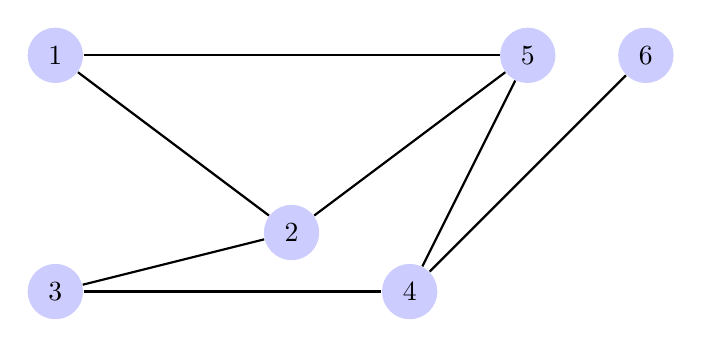
\begin{tikzpicture}[scale=1.5, auto,swap]
    % Vertices
    \foreach \pos/\name in {{(0,2)/1}, {(2,0.5)/2}, {(0,0)/3}, {(3,0)/4}, {(4,2)/5}, {(5,2)/6}}
        \node[vertex] (\name) at \pos {$\name$};
    
    % Edges
    \foreach \source/ \dest in {1/2, 1/5, 2/5, 2/3, 3/4, 4/5, 4/6}
        \path[edge] (\source) -- (\dest);
\end{tikzpicture}
\end{center}

\subsection*{Adjacency Matrix of the Example Graph}
The adjacency matrix \( A \) for the undirected graph \( G \) is:
\[ A = \begin{bmatrix}
0 & 1 & 0 & 0 & 1 & 0 \\
1 & 0 & 1 & 0 & 1 & 0 \\
0 & 1 & 0 & 1 & 0 & 0 \\
0 & 0 & 1 & 0 & 1 & 1 \\
1 & 1 & 0 & 1 & 0 & 0 \\
0 & 0 & 0 & 1 & 0 & 0
\end{bmatrix} \]
\section{Pagerank Algorithm}
The PageRank algorithm measures the importance of each node within a graph. It gives the idea that connections to high-importance nodes contribute more to the importance of the node in question. This importance is quantified through a vector \( \mathbf{u} \), where each entry \( u_i \) corresponds to the centrality (importance) of node \( i \).

\subsection*{Centrality and Eigenvector Problem}
The centrality of a node is not just a function of its degree \( d_i \), but also the centralities of the nodes pointing to it. The centrality \( u_i \) for node \( i \) can be expressed as:
\[ u_i = \sum_{j=1}^{n} a_{ij}u_j \]

This is the sum of the connection weights to a nodes other neighbours, multiplied by the importance of the neighbour, which can be performed by matrix operation $A\textbf{u}$. When optimising for the weights, we expect to reach convergence when we iteratively solve this eigenvector problem:
\[ A\mathbf{u} = \lambda \mathbf{u} \]
where \( A \) is the adjacency matrix of the graph, and \( \lambda \) is a constant. This is an eigenvalue problem, because given an adjacency matrix \textbf{A} and a vector \textbf{u} of correct importance scores for the given \textbf{A}, their product (which is an act of calculating importance scores) should still net the same \textbf{u}. This makes \textbf{u} the principal eigenvector that gives the centrality scores. We want the entries of \textbf{u} to be non-negative, so we want the largest eigenvalue of A (proof for this is not shown).

\subsection*{Power Method for PageRank}
To find the principal eigenvector, the Power Method is utilised:
\begin{enumerate}
     \item Assume matrix $\textbf{A}$ with a full set of eigenvectors $(\textbf{u}_1, \textbf{u}_2, ... \textbf{u}_n)$ and no multiple eigenvalues.
     \item Start with a non-negative initial guess vector \( \mathbf{x}_0 \).
    \item Iterate \( \mathbf{x}_{k} = \frac{A\mathbf{x}_{k-1} }{||A\mathbf{x}_{k-1} ||}\), and normalise \( \mathbf{x}_{k} \) at each step to prevent divergence. It is not specified in the notes which norm to use (it is assumed to be the L2 norm following the notation of the module), some other practices take the infinity norm which is the largest component in the vector.
\end{enumerate}
As \( k \) approaches infinity, \( \mathbf{x}_{k} \) converges to the principal eigenvector \( \mathbf{u} \), corresponding to the largest eigenvalue, which is used as the PageRank score.\\

This is because 

\[\textbf{x}_k=\textbf{Ax}_{k-1}=\textbf{A}^\textbf{k}\textbf{x}_0=U\Lambda^kU^{-1}x_0=c_1\lambda_1^ku_1+c_2\lambda_2^ku_2+\cdots+c_n\lambda_n^ku_n\]

Expanding the equation:

\[
\mathbf{x}_k = U\Lambda^kU^{-1}\mathbf{x}_0 = 
\begin{bmatrix}
| & | & & | \\
\mathbf{u}_1 & \mathbf{u}_2 & \cdots & \mathbf{u}_n \\
| & | & & |
\end{bmatrix}
\begin{bmatrix}
\lambda_1^k & 0 & \cdots & 0 \\
0 & \lambda_2^k & \cdots & 0 \\
\vdots & \vdots & \ddots & \vdots \\
0 & 0 & \cdots & \lambda_n^k
\end{bmatrix}
\begin{bmatrix}
| & | & & | \\
\mathbf{u}_1 & \mathbf{u}_2 & \cdots & \mathbf{u}_n \\
| & | & & |
\end{bmatrix}^{-1}
\mathbf{x}_0
\]

The eigenvalues \( \lambda_i \) are typically ordered such that \( |\lambda_1| \geq |\lambda_2| \geq \cdots \geq |\lambda_n| \), and the coefficients \( c_i \) are the components of \( \mathbf{x}_0 \) in the basis of eigenvectors \( \mathbf{u}_i \). As \( k \) increases, \( \lambda_1^k \) dominates the sum, and \( \mathbf{x}_k \) converges to a scalar multiple of the principal eigenvector \( \mathbf{u}_1 \):

\[
\mathbf{x}_k \approx c_1\lambda_1^k\mathbf{u}_1
\]

where \( c_1 \) is the component of the initial guess \( \mathbf{x}_0 \) in the direction of \( \mathbf{u}_1 \).


Note that this algorithm is standard, not too performant, but works for manual calculation.

\subsection*{Example Application of PageRank}
Considering our graph \( G \) with nodes \( \{1,2,3,4,5,6\} \) and edges \( \{(1,2), (1,5), (2,5), (4,5), (2,3), (3,4), (4,6)\} \), let us calculate the PageRank scores.

\subsubsection*{Graph Representation}
The graph is represented as:

\begin{center}
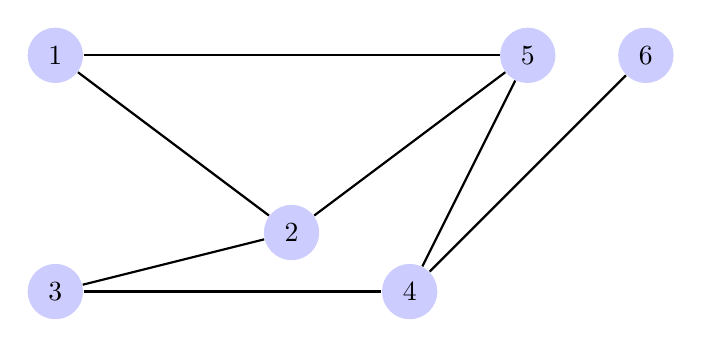
\begin{tikzpicture}[scale=1.5, auto,swap]
    % Vertices
    \foreach \pos/\name in {{(0,2)/1}, {(2,0.5)/2}, {(0,0)/3}, {(3,0)/4}, {(4,2)/5}, {(5,2)/6}}
        \node[vertex] (\name) at \pos {$\name$};
    
    % Edges
    \foreach \source/ \dest in {1/2, 1/5, 2/5, 2/3, 3/4, 4/5, 4/6}
        \path[edge] (\source) -- (\dest);
\end{tikzpicture}
\end{center}

\subsubsection*{Adjacency Matrix and PageRank Scores}

We start with initial guess $\textbf{x}_0$
\[\textbf{x}_0=\begin{bmatrix}
    1\\1\\1\\1\\1\\1
\end{bmatrix}\ \text{and }  \textbf{A} = \begin{bmatrix}
0 & 1 & 0 & 0 & 1 & 0 \\
1 & 0 & 1 & 0 & 1 & 0 \\
0 & 1 & 0 & 1 & 0 & 0 \\
0 & 0 & 1 & 0 & 1 & 1 \\
1 & 1 & 0 & 1 & 0 & 0 \\
0 & 0 & 0 & 1 & 0 & 0
\end{bmatrix}\]

\[ \textbf{x}_1 = \textbf{Ax}_0 \begin{bmatrix}
0 & 1 & 0 & 0 & 1 & 0 \\
1 & 0 & 1 & 0 & 1 & 0 \\
0 & 1 & 0 & 1 & 0 & 0 \\
0 & 0 & 1 & 0 & 1 & 1 \\
1 & 1 & 0 & 1 & 0 & 0 \\
0 & 0 & 0 & 1 & 0 & 0
\end{bmatrix}\begin{bmatrix}
    1\\1\\1\\1\\1\\1
\end{bmatrix} = 
\begin{bmatrix}
    2\\3\\2\\3\\3\\1
\end{bmatrix} \rightarrow_{\text{normalise}} 
\begin{bmatrix}
0.3333 \\ 0.5000 \\ 0.3333 \\ 0.5000 \\ 0.5000 \\ 0.1667
\end{bmatrix}
\]
\[
\textbf{x}_2 = \textbf{Ax}_1 = \begin{bmatrix}
0 & 1 & 0 & 0 & 1 & 0 \\
1 & 0 & 1 & 0 & 1 & 0 \\
0 & 1 & 0 & 1 & 0 & 0 \\
0 & 0 & 1 & 0 & 1 & 1 \\
1 & 1 & 0 & 1 & 0 & 0 \\
0 & 0 & 0 & 1 & 0 & 0
\end{bmatrix}\begin{bmatrix}
0.333 \\ 0.500 \\ 0.333 \\ 0.500 \\ 0.500 \\ 0.167
\end{bmatrix} \rightarrow_{\text{normalise}}
\begin{bmatrix}
0.396 \\ 0.462 \\ 0.396 \\ 0.396 \\ 0.528 \\ 0.198
\end{bmatrix}
\]

\begin{align*}
\textbf{x}_3=\textbf{Ax}_2 = \begin{bmatrix}
0 & 1 & 0 & 0 & 1 & 0 \\
1 & 0 & 1 & 0 & 1 & 0 \\
0 & 1 & 0 & 1 & 0 & 0 \\
0 & 0 & 1 & 0 & 1 & 1 \\
1 & 1 & 0 & 1 & 0 & 0 \\
0 & 0 & 0 & 1 & 0 & 0
\end{bmatrix}\begin{bmatrix}
0.396 \\ 0.462 \\ 0.396 \\ 0.396 \\ 0.528 \\ 0.198
\end{bmatrix} \rightarrow_{\text{normalise}}
\begin{bmatrix}
0.390 \\ 0.520 \\ 0.338 \\ 0.442 \\ 0.494 \\ 0.156
\end{bmatrix}\\
\vdots \quad \quad \\
\textbf{x}_{50} = \begin{bmatrix}0.401\\0.502\\0.358\\0.408\\0.516\\0.160\end{bmatrix}
\end{align*}

It does follow after many iterations that node 2 and node 5 are the two most central nodes in this network, and it is notable that they both are linked together and have the highest number of connections, 3. Although node 4 has 3 connections as well, it is connected to nodes of lesser importance, resulting in a lower rank.











\chapter{Solving $\textbf{Ax = b}$}
\section{Interpretations}

We aim to solve $\textbf{Ax} = \textbf{b}$ where $b \in \mathbb{C}^m$ and $\textbf{A} \in \mathbb{C}^{m\times n}$, and we want to determine if solution $\textbf{x}$ exists and whether it is unique. \\

Otherwise, if there is no solution, we pick the best approximation. We are also interested when $m\neq n $, when there is no solutions, or if they are not unique.\\

Estimating $\textbf{x}$ from $\textbf{Ax} = \textbf{b}$ is an inverse problem. An example in engineering: when the equations in $\textbf{A}$ models a distortion filter operation on some data, and we want to want restore $\textbf{x}$. An example of distortion could be motion blur in a photo, or room echo in a sound recording.\\

\begin{figure}[H]
    \centering
    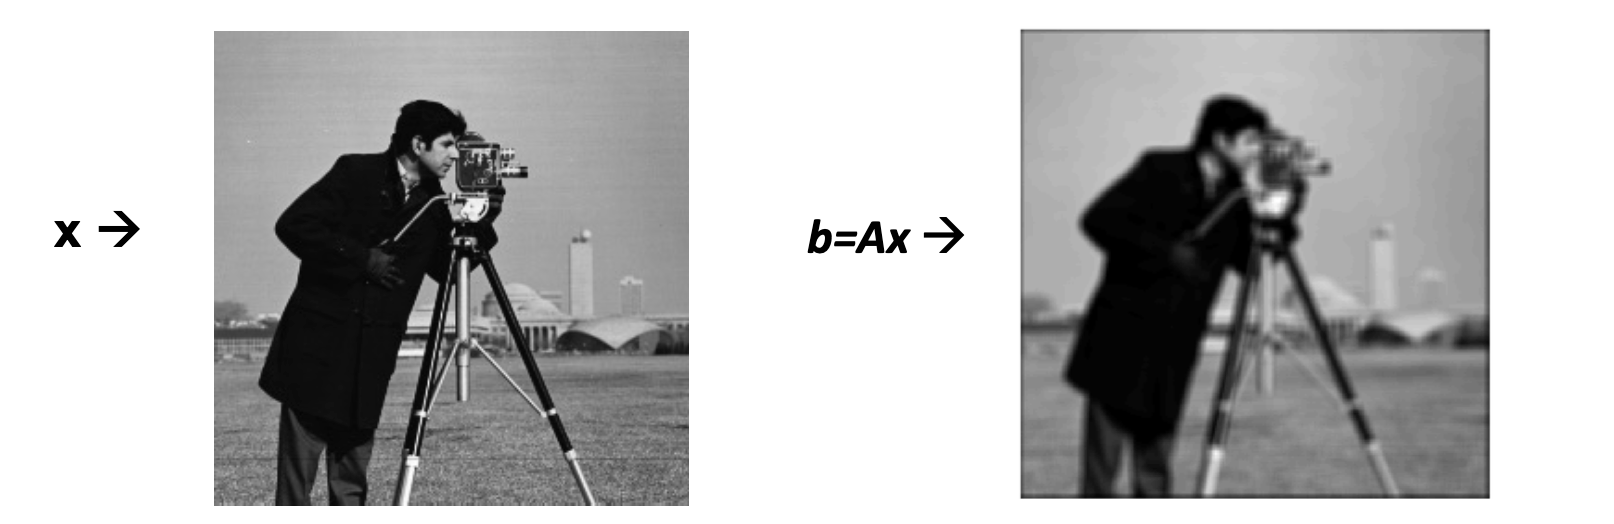
\includegraphics[width=0.7\linewidth]{img/conv_blur.png}
    
    
\end{figure}

\subsubsection*{Geometric Interpretation}
In the context of linear algebra, the equation \(Ax = b\) can be interpreted in both pure mathematical and geometrical terms as a system of linear equations. 

\begin{itemize}
    \item When \(m = n\), we have an equal number of equations and unknowns, which constitutes a square system. For instance, consider the system
    \[
    \begin{pmatrix}
    1 & 2 \\
    1 & -1 \\
    \end{pmatrix}
    \begin{pmatrix}
    x_1 \\
    x_2 \\
    \end{pmatrix}
    =
    \begin{pmatrix}
    4 \\
    1 \\
    \end{pmatrix},
    \]
    where each equation represents a line in a two-dimensional space. The intersection of two non-parallel lines signifies a unique solution.

    \item If the lines represented by the equations are parallel, the system may either have no solution or infinitely many solutions (the lines coincide). The \emph{rank} of matrix \(A\) is a critical determinant in identifying the uniqueness of the solution.

    \item In the case where \(m > n\), implying more equations than unknowns, the system is referred to as `tall'. Generally, such systems do not have a unique solution, as the equations may intersect at multiple points unless several of them overlap.

    \item Conversely, when \(m < n\), meaning there are more unknowns than equations, the system is described as `fat'. An example of this is when \(m = 2\) and \(n = 3\); we are dealing with two planes in a three-dimensional space. Unless the planes are parallel, they intersect along a line, leading to an infinite number of solutions. Thus, the solution, if it exists, is not unique.
\end{itemize}
\subsubsection*{Vector Space Interpretation}

Consider the matrix equation \( \mathbf{Ax} = \mathbf{b} \). This can be interpreted within the framework of vector spaces as follows:

\begin{itemize}
    \item The matrix \( \mathbf{A} \) can be seen as a linear transformation that maps vectors from \( \mathbb{C}^n \) to \( \mathbb{C}^m \).
    \item The operation \( \mathbf{Ax} \) corresponds to forming linear combinations of the columns of \( \mathbf{A} \), where the vector \( \mathbf{x} \) provides the combination coefficients.
    \item A solution to \( \mathbf{Ax} = \mathbf{b} \) is feasible if and only if the vector \( \mathbf{b} \) resides within the range (or column space) of \( \mathbf{A} \).
    \item The range space of \( \mathbf{A} \), denoted as \( \mathcal{R}(\mathbf{A}) \), contains all possible vectors \( \mathbf{b} \) that can be reached by the linear transformation \( \mathbf{A} \). If \( \mathcal{R}(\mathbf{A}) = \mathbb{C}^m \), meaning \( \mathbf{A} \) has full row rank, then any vector in \( \mathbb{C}^m \) can be obtained from \( \mathbf{A} \).
    \item {\color{green!55!blue}The existence of a solution is indicated by \( \mathbf{b} \) being in the range space of \( \mathbf{A} \), while the null space of \( \mathbf{A} \) determines the uniqueness. Specifically, if the null space of \( \mathbf{A} \) contains only the zero vector (is trivial), the solution to \( \mathbf{Ax} = \mathbf{b} \) is unique.}
    \item {\color{green!55!blue}Conversely, if the null space of \( \mathbf{A} \) is non-trivial, possessing vectors other than the zero vector, multiple solutions to \( \mathbf{Ax} = \mathbf{b} \) may exist.}
\end{itemize}


\section{Existence and Uniqueness}
The previous section is summarised by these theorems:

\begin{theorembox}{Existence}
Let $\textbf{A} \in \mathbb{C}^{m\times n}$.
\begin{enumerate}
    \item For each $\textbf{b} \in \mathbb{C}^m$ there exists at least one solution $\textbf{Ax}=\textbf{b}$
    \item The range space of \textbf{A} is full: $\mathcal{R}(\textbf{A}) = \mathbb{C}^m$
    \item $rank(\textbf{A}) = m$
    \item \textbf{A} is full row rank, so its rows are linearly independent.
These conditions imply $m\leq n$, a fat or square matrix.
\end{enumerate}
\end{theorembox}
\begin{theorembox}{Uniqueness}
Let $\textbf{A} \in \mathbb{C}^{m\times n}$.
\begin{enumerate}
    \item If there exists a solution to $\textbf{Ax}=\textbf{b}$,it is unique
    \item The null space of \textbf{A} is trivial (containing nothing but the zero vector)
    \item $rank(\textbf{A}) = n$
    \item \textbf{A} is full column rank, so its columns are linearly independent.
\end{enumerate}
These conditions imply $m\geq n$, a tall or square matrix.
\end{theorembox}

\begin{theorembox}{Existence and Uniqueness}
Let $\textbf{A} \in \mathbb{C}^{m\times n}$.
\begin{enumerate}
    \item For each $\textbf{b} \in \mathbb{C}^m$ there exists at least one solution $\textbf{Ax}=\textbf{b}$ and it is unique
    \item The range space of \textbf{A} is $m$: $\mathcal{R}(\textbf{A}) = \mathbb{C}^m$
    \item $rank(\textbf{A}) = m = n$ and \textbf{A}'s null space is trivial.
    \item \textbf{A} is square and nonsingular, so it has a determinant $\neq 0$
\end{enumerate}
\end{theorembox}

\begin{enumerate}
    \item Consider the matrix 
    \[
    A = \begin{pmatrix}
    4 & 8 & 6 \\
    0 & 4 & 7
    \end{pmatrix}.
    \]
    The rows are linearly independent, so for every vector \( \mathbf{b} \) in \( \mathbb{C}^2 \), there is at least one solution to \( A\mathbf{x} = \mathbf{b} \).

    \item The matrix
    \[
    A = \begin{pmatrix}
    1 & 0 & 1 \\
    0 & 1 & 1 \\
    1 & 1 & 2
    \end{pmatrix}
    \]
    has three rows but only rank 2. The conditions for the existence theorem are not satisfied, and there exist vectors \( \mathbf{b} \) for which \( A\mathbf{x} = \mathbf{b} \) has no solution. For example, \( \mathbf{b} = \begin{pmatrix} 0 & 0 & 1 \end{pmatrix}^\text{T} \).

    \item The matrix
    \[
    A = \begin{pmatrix}
    6 & 5 & 6 & 3 \\
    2 & 3 & 0 & 1 \\
    4 & 4 & 3 & 2
    \end{pmatrix}
    \]
    has more columns than rows and is not full row rank. Thus, the conditions for the existence theorem are not met, and a solution to \( A\mathbf{x} = \mathbf{b} \) does not always exist. Remember, having 'more unknowns than equations' or being 'underdetermined' does not guarantee the existence of a solution; having 'full row rank' does.
    \item Given the matrix 
\[ A = \begin{pmatrix} 0 & 1 \\ 1 & 1 \\ 1 & 0 \end{pmatrix}, \]
the columns are linearly independent. Therefore, for every vector \( \mathbf{b} \) in \( \mathbb{C}^2 \), there exists a unique solution to \( A\mathbf{x} = \mathbf{b} \). For example, if \( \mathbf{b} = \begin{pmatrix} 4 \\ 6 \\ 2 \end{pmatrix} \), the unique solution is \( \mathbf{x} = \begin{pmatrix} 2 \\ 4 \end{pmatrix} \). However, for \( \mathbf{b} = \begin{pmatrix} 1 \\ 0 \\ 0 \end{pmatrix} \), no solution exists.
    \item For the matrix 
\[ A = \begin{pmatrix} 1 & 0 & 1 \\ 0 & 1 & 1 \\ 1 & 1 & 2 \end{pmatrix}, \]
the columns are linearly dependent, with the null space being the span of \( \begin{pmatrix} 1 \\ 1 \\ -1 \end{pmatrix} \). Thus, neither uniqueness nor existence of the solution is guaranteed.
    \item Consider the matrix 
\[ A = \begin{pmatrix} 2 & 5 & 3 \\ 3 & 5 & 2 \\ 3 & 7 & 4 \\ 7 & 8 & 1 \end{pmatrix}. \]
The columns are linearly dependent, which means that even though the system is overdetermined, uniqueness of the solution cannot be assured.

\end{enumerate}

Our goal is to develop a single method that either finds \textbf{x} as the solution to $\textbf{Ax}=\textbf{b}$ if it exists, or find the best approximation.
\section{Four Fundamental Subspaces}
Given a linear mapping $A: \mathbb{C}^n \rightarrow \mathbb{C}^m$ represented by the matrix $A \in \mathbb{C}^{m \times n}$, we consider two important concepts: the range (or column space) of $A$, denoted as $\mathcal{R}(A)$, and the null space (or kernel) of $A$, denoted as $\mathcal{N}(A)$.

Exploring further, let us examine the adjoint of $A$, denoted as $A^H$, which maps vectors from $\mathbb{C}^m$ to $\mathbb{C}^n$. It is crucial to understand that $A^H$ is not necessarily the inverse of $A$ but rather the conjugate transpose of $A$.

The range of $A^H$, $\mathcal{R}(A^H)$, and the null space of $A^H$, $\mathcal{N}(A^H)$, can be defined analogously. These subspaces interact with each other in the following ways, which we state without proof:

\begin{itemize}
  \item $\mathbb{C}^m = \mathcal{R}(A) \oplus \mathcal{N}(A^H)$, where $\oplus$ denotes the direct sum, and $\mathcal{R}^\perp(A) = \mathcal{N}(A^H)$, meaning the orthogonal complement of the range of $A$ is the null space of $A^H$.
  \item $\mathbb{C}^n = \mathcal{R}(A^H) \oplus \mathcal{N}(A)$, and $\mathcal{R}^\perp(A^H) = \mathcal{N}(A)$, indicating that the orthogonal complement of the range of $A^H$ is the null space of $A$.
\end{itemize}


\begin{figure}[H]
    \centering
    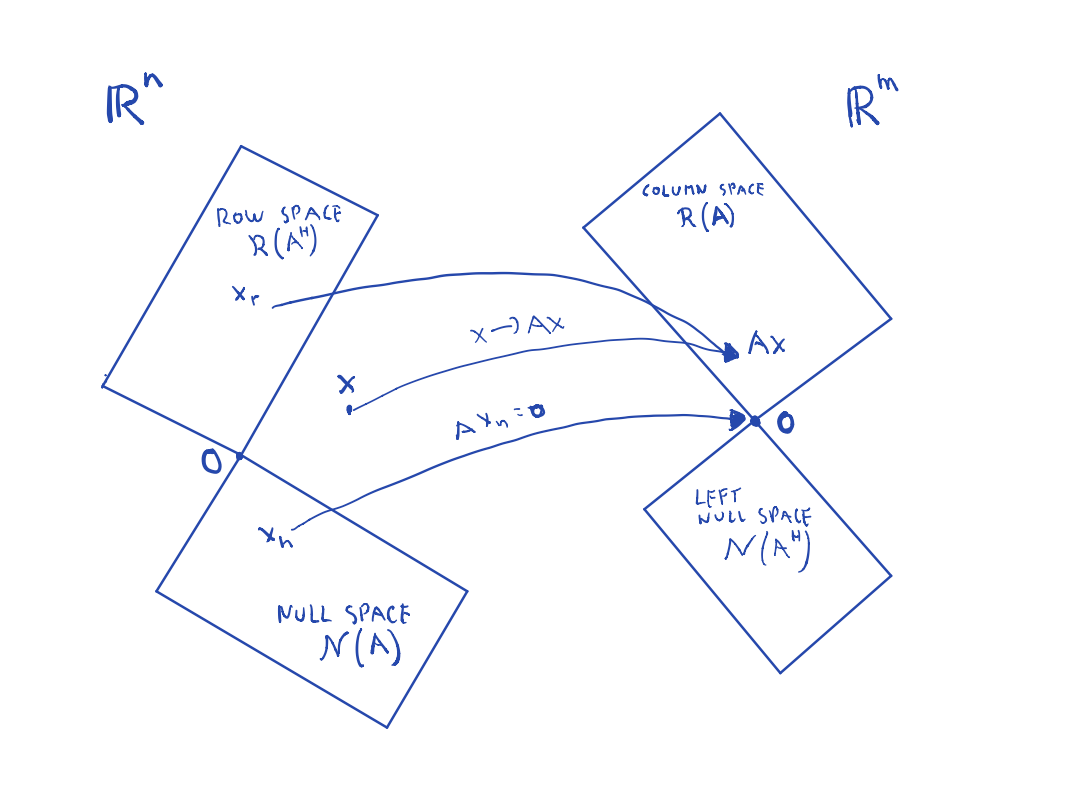
\includegraphics[width=0.75\linewidth]{img/subspaces.png}
    \caption{Visual representation of the four fundamental subspaces in linear algebra. The null space and row space are mapped through $A$ and $A^H$ to the column space and left null space respectively. Each vector in the null space maps to the zero vector in the column space, while vectors in the row space and beyond map into the column space. Would be nice to replace this with an actual diagram, will do this when I have more time}
\end{figure}

\begin{examplebox}{Sample subspaces question}
    Consider the matrix 
\[
A = \begin{pmatrix}
1 & 1 & 1 \\
0 & 1 & 0 \\
0 & 0 & 0 \\
\end{pmatrix}.
\]
Our goal is to find the four fundamental subspaces of $A$: the column space $\mathcal{R}(A)$, the null space $\mathcal{N}(A)$, the row space $\mathcal{R}(A^H)$, and the left null space $\mathcal{N}(A^H)$.

\subsubsection*{Column Space and Null Space}
Since $A$ is already in row-echelon form, the range space (or column space) of $A$ is spanned by the first two columns of $A$:
\[
\mathcal{R}(A) = \text{span}\left\{ \begin{pmatrix} 1 \\ 0 \\ 0 \end{pmatrix}, \begin{pmatrix} 1 \\ 1 \\ 0 \end{pmatrix} \right\}.
\]
The dimension of the null space of $A$ is given by the Rank-Nullity Theorem:
\[
\dim(\mathcal{N}(A)) = 3 - \text{rank}(A) = 1.
\]
A basis for the null space, found by solving $A\bm{n} = \bm{0}$, is:
\[
\mathcal{N}(A) = \text{span}\left\{ \begin{pmatrix} 1 \\ 0 \\ -1 \end{pmatrix} \right\}.\]

\subsubsection*{Row Space and Left Null Space}
The row space of $A^H$, which is the column space of $A$, has already been determined. The left null space is the orthogonal complement of the row space in $\mathbb{C}^m$:
\[
\mathcal{N}(A^H) = \text{span}\left\{ \begin{pmatrix} 0 \\ 0 \\ 1 \end{pmatrix} \right\}.
\]
Finally, the row space of $A$ (which is the column space of $A^H$) can be obtained by taking the non-zero rows of $A$:
\[
\mathcal{R}(A^H) = \text{span}\left\{ \begin{pmatrix} 1 \\ 1 \\ 1 \end{pmatrix}, \begin{pmatrix} 0 \\ 1 \\ 0 \end{pmatrix} \right\}.
\]
\end{examplebox}


 \section{Inverses}
 We classify inverses of matrices based on their dimensions and rank:

\begin{itemize}
    \item A square and nonsingular (invertible) matrix $A$ possesses an inverse $A^{-1}$ such that $AA^{-1} = A^{-1}A = I$, where $I$ is the identity matrix.
    \item Non-square matrices do not have an inverse in the traditional sense; however, they may have a left or right inverse under certain conditions:
    \begin{itemize}
        \item A \textbf{left inverse} of a matrix $A$ exists if there is a matrix $B$ such that $BA = I$ (and typically $AB \neq I$), which requires $A$ to be full column rank.
        \item A \textbf{right inverse} of a matrix $A$ exists if there is a matrix $C$ such that $AC = I$, necessitating $A$ to be full row rank.
    \end{itemize}
    \item It is important to note that these inverses may not be unique.
\end{itemize}


 
\section{Projections and Approximations}
\begin{theorembox}{Projection Theorem}
Let \( V \) be a closed subspace of Hilbert space \( H \) and let \( x \) be a vector in \( H \).
\begin{enumerate}
  \item \textbf{Existence:} There exists \( \hat{x} \in V \) such that \( \|x - \hat{x}\| \leq \|x - v\| \) for all \( v \in V \).
  \item \textbf{Orthogonality:} \( x - \hat{x} \perp V \) is necessary and sufficient for determining \( \hat{x} \).
  \item \textbf{Uniqueness:} The vector \( \hat{x} \) is unique.
  \item \textbf{Linearity:} \( \hat{x} = Px \) where \( P \) is a linear operator that depends on \( V \) and not on \( x \).
  \item \textbf{Idempotency:} \( P(Px) = Px \) for all \( x \in H \).
  \item \textbf{Self-adjointness:} \( P = P^H \).
\end{enumerate}
\end{theorembox}

\begin{definitionbox}{Projection Matrix}
    Given a matrix \( A \) and a vector \( \mathbf{b} \), we seek to project \( \mathbf{b} \) onto the column space of \( A \). The projection is denoted by \( A\mathbf{x} \), where \( \mathbf{x} \) is the vector in the column space of \( A \) that is closest to \( \mathbf{b} \).

\subsection*{Orthogonality Principle}
The difference \( \mathbf{b} - A\mathbf{x} \) is orthogonal to the column space of \( A \), implying that it lies in the null space of \( A^T \). Hence, we have:
\begin{equation}
    A^T(\mathbf{b} - A\mathbf{x}) = 0
\end{equation}

\subsection*{Derivation}
Rearranging the above equation, we obtain:
\begin{align}
    A^T\mathbf{b} &= A^TA\mathbf{x} \\
    \Rightarrow \mathbf{x} &= (A^TA)^{-1}A^T\mathbf{b}
\end{align}
This equation provides us with the least squares solution for \( \mathbf{x} \).

\subsection*{Projection Matrix}
The matrix that projects any vector \( \mathbf{b} \) onto the column space of \( A \) is known as the projection matrix, \( P \), and is given by:
\begin{equation}
    P = A(A^TA)^{-1}A^T
\end{equation}
This projection matrix has the property that \( P\mathbf{b} = A\mathbf{x} \), which is the projection of \( \mathbf{b} \) onto the column space of \( A \).

\begin{figure}[H]
    \centering
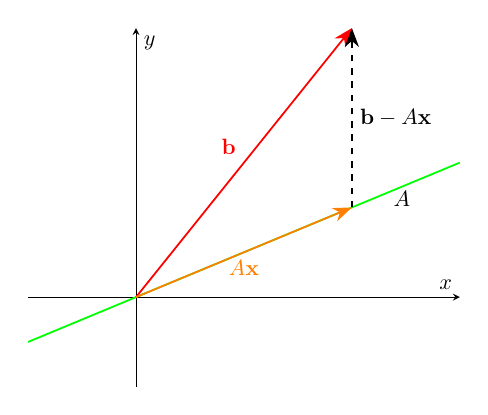
\begin{tikzpicture}[scale=0.8, >=Stealth]
    \begin{axis}[
        axis lines=middle,
        xmin=-1, xmax=3,
        ymin=-1, ymax=3,
        xlabel={$x$},
        ylabel={$y$},
        xtick={0}, ytick={0},
        xticklabels={,,}, yticklabels={,,}
    ]

    % Line A passing through the origin
    \addplot[domain=-1:3, samples=2, green, thick] {0.5*x};
    \node[label={0:{\(A\)}}, inner sep=0pt] at (axis cs:2.3,1.1) {};

    % Vector b
    \draw[red, thick, -{>[length=3mm]}] (0,0) -- (2,3) node[midway, above left] {\(\mathbf{b}\)};

    % Projection of b onto A (Ax)
    \draw[orange, thick, -{>[length=3mm]}] (0,0) -- (2,1) node[midway, below] {\(A\mathbf{x}\)};

    % Error vector b - Ax
    \draw[black, dashed, thick, -{>[length=3mm]}] (2,1) -- (2,3) node[midway, right] {\(\mathbf{b} - A\mathbf{x}\)};

    \end{axis}
\end{tikzpicture}
\end{figure}
 
\end{definitionbox}
\section{Gram-Schmidt Orthogonalisation Process}


The Gram-Schmidt process is a method for orthonormalising a set of vectors in an inner product space. It is a direct application of the projection theorem, and it helps to form an orthonormal basis, which is a cornerstone in linear algebra and has crucial applications in signal processing and systems theory.

\subsection*{Orthogonal and Orthonormal Matrices}

At the outset of our course, we discussed orthogonal matrices. Now, we delve into a practical use-case of these concepts.

\begin{itemize}
    \item An \textbf{orthogonal matrix} $A$ is a square matrix with real entries whose columns and rows are orthonormal vectors. That is, the transpose of $A$ is also its inverse: $A^\mathsf{T}A = AA^\mathsf{T} = I$, where $I$ is the identity matrix. 
    \item When we construct a matrix $A$ from a set of vectors $\{v_i\}_{i=1}^n$ that form an orthonormal basis, it satisfies this property. 
    \item Mathematically, if $v_i$ for $i = 1, 2, \ldots, n$ are orthonormal, then:
    \begin{equation}
        A = \begin{pmatrix}
            v_{1,1} & \cdots & v_{1,n} \\
            \vdots & \ddots & \vdots \\
            v_{n,1} & \cdots & v_{n,n}
        \end{pmatrix}
    \end{equation}
    \item Such matrices not only preserve lengths (due to maintaining the induced norm) but also angles between vectors when used in linear transformations.
\end{itemize}

\subsection*{The Process}

The essence of the Gram-Schmidt process is to take a set of linearly independent vectors and orthogonalise them while maintaining their span.

\begin{itemize}
    \item Start with any set of independent vectors $\{a, b, c\}$.
    \item First normalise vector $a$ to find $q_1$:
    \begin{equation}
        q_1 = \frac{a}{\|a\|}
    \end{equation}
    \item To find $q_2$, orthogonal to $q_1$, project $b$ onto $q_1$ and subtract this projection from $b$, then normalise:
    \begin{equation}
        q_2 = \frac{b - \text{proj}_{q_1}(b)}{\|b - \text{proj}_{q_1}(b)\|}
    \end{equation}
    \item The projection operator $P$ onto $q_1$ is defined as:
    
    \begin{equation}
        P = \frac{a a^\mathsf{T}}{a^\mathsf{T}a}
    \end{equation}
    \item For vector $c$, ensure it is orthogonal to both $q_1$ and $q_2$:
    \begin{equation}
        q_3 = \frac{c - \text{proj}_{q_1}(c) - \text{proj}_{q_2}(c)}{\|c - \text{proj}_{q_1}(c) - \text{proj}_{q_2}(c)\|}
    \end{equation}
    \item This process can be continued for higher dimensions. If there were a fourth vector $d$, we would subtract its projections onto $q_1$, $q_2$, and $q_3$ before normalizing.
\end{itemize}

\subsection*{Visualising the Concept}

Consider vectors $a$, $b$, and $c$ in a three-dimensional space. By applying the Gram-Schmidt process, we are essentially rotating and stretching the axes of our coordinate system such that each vector $q_i$ lies along one of these new axes, ensuring orthogonality and normality.

\begin{itemize}
    \item Visual representation of transforming vector $b$:
    \begin{equation}
        B = b - \frac{a a^\mathsf{T}}{a^\mathsf{T}a}b
    \end{equation}
    \item This transformed vector $B$ is now orthogonal to $a$.
    \item We then apply a similar approach to vector $c$ to ensure it is orthogonal to both $a$ and $B$:
    \begin{equation}
        C = c - \frac{a a^\mathsf{T}}{a^\mathsf{T}a}c - \frac{b b^\mathsf{T}}{b^\mathsf{T}b}c
    \end{equation}
\end{itemize}
Make sure to normalise the vectors after their transformations!\\
\textbf{In general we subtract from every new vector its projections in the directions already set.} Then we make the resulting vectors orthonormal, by dividing the vectors with their magnitudes.

\subsection*{Remarks}

The Gram-Schmidt process is an elegant way of generating an orthogonal set from a linearly independent set. It plays a significant role in many areas of mathematics and engineering, including the understanding of Fourier series, signal processing, and the method of least squares in statistics.

\section{Solutions, either exact or approximate}
% We take the derivative and set it to zero.\\


Let's consider the problem of finding a vector \( \mathbf{x} \) such that \( A\mathbf{x} = \mathbf{b} \), with a particular focus on matrices \( A \) that have full column rank.

\begin{itemize}
    \item A matrix \( A \) with full column rank is tall, implying that the columns of \( A \) are linearly independent. If a solution to the system \( A\mathbf{x} = \mathbf{b} \) exists, this solution is unique due to the full column rank of \( A \).
    
    \item To solve the system, we aim to find the left inverse of \( A \). This is because the left inverse allows us to compute the solution directly for a full column rank matrix.
    
    \item The solution process involves a somewhat convoluted but geometrically inspired approach. We seek a vector \( \mathbf{x}_{LS} \) that minimizes the norm \( \|A\mathbf{x}_{LS} - \mathbf{b}\| \), making it the least squares solution. This means that \( \|A\mathbf{x}_{LS} - \mathbf{b}\| \leq \|A\mathbf{x} - \mathbf{b}\| \) for any vector \( \mathbf{x} \).
    
    \item Consequently, if a solution to \( A\mathbf{x} = \mathbf{b} \) exists, then \( \mathbf{x}_{LS} \) is that solution, and it can be found by projecting \( \mathbf{b} \) onto the column space of \( A \).
\end{itemize}


\textbf{Claim:}

The vector $\widehat{x}$ minimises $||Ax-b||$ iff $A^H A\widehat{x} = A^Hb$, which is the normal equation.\\


\textbf{Proof:}
\begin{itemize}
    \item Minimizing $\|Ax - b\|$ is equivalent to minimizing $\|\hat{b} - b\|$ where $\hat{b} \in \mathcal{R}(A)$.
    \item By the projection theorem: $b - \hat{b} \in \mathcal{R}(A)^\perp \Rightarrow b - \hat{b} \in \mathcal{N}(A^H)$.
    \item Therefore, $A^H(b - \hat{b}) = 0 \Rightarrow A^Hb = A^H\hat{b} \Rightarrow A^HA\hat{x} = A^Hb$.
    \item Conversely $A^HA\hat{x} = A^Hb \Rightarrow A^H(b - A\hat{x}) = 0$.
\end{itemize}
\begin{figure}
    \centering
    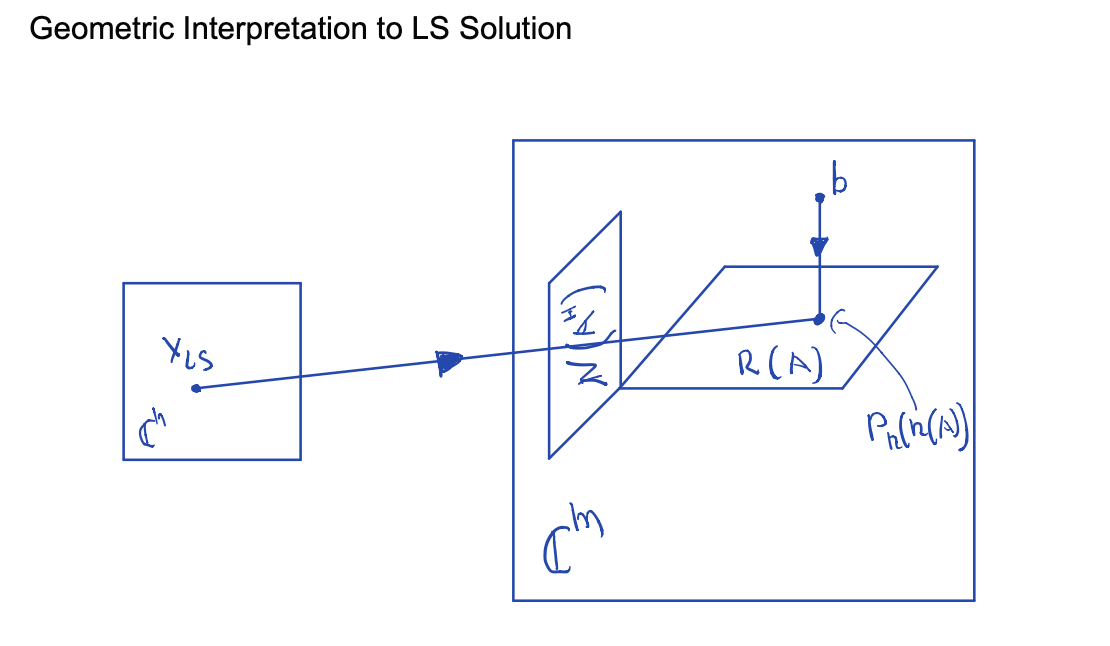
\includegraphics[width=0.75\linewidth]{img/geom_ls.png}
    
    
\end{figure}

% \begin{examplebox}{Title}
%     \begin{align*}
%     ||Ax = b|| \Rightarrow \\
%     \left| \left| \begin{pmatrix}
%         a_{11} & a_{12} \\
%         a_{21} & a_{22} \\
%     \end{pmatrix}
%     \begin{pmatrix}
%         x_1 \\ x_2
%     \end{pmatrix} =
%     \begin{pmatrix}
%         b_1 \\ b_2
%     \end{pmatrix}\right| \right| 
%     \end{align*}
% \end{examplebox}
\subsection{Example: Least-Square Deconvolution}
Assume you have a system that blurs an image, this is your FIR (finite impulse response) filter. You want to recover the original sharp image. However, this observed image is noisy. Using the deconvolution process, you would attempt to reverse the blurring to approximate the original image as closely as possible.\\

Given the output $\textbf{y}\in \mathbb{C}^{n+k-1}$ of the filter and the filter is represented by matrix $\textbf{A} \in \mathbb{C}^{(n+k-1)\times n}$, which is the convolution (Toeplitz) matrix associated with K-tap filter $\textbf{h}$. Each row of the Toeplitz matrix is a shifted version of the filter coeffficients (or taps).\\

If $\textbf{y}$ is noise-free, we can find the signal easily, but it is usually noisy. So we have the measured signal $\textbf{b} = \textbf{y}+\textbf{n}$ \\

We can solve for $\textbf{A}^H \textbf{A}\hat{\textbf{x}} = \textbf{A}^H\textbf{b}$, to get $\hat{\textbf{x}}$ that is the closest to the true signal \textbf{x}.

\begin{figure}[H]
    \centering
    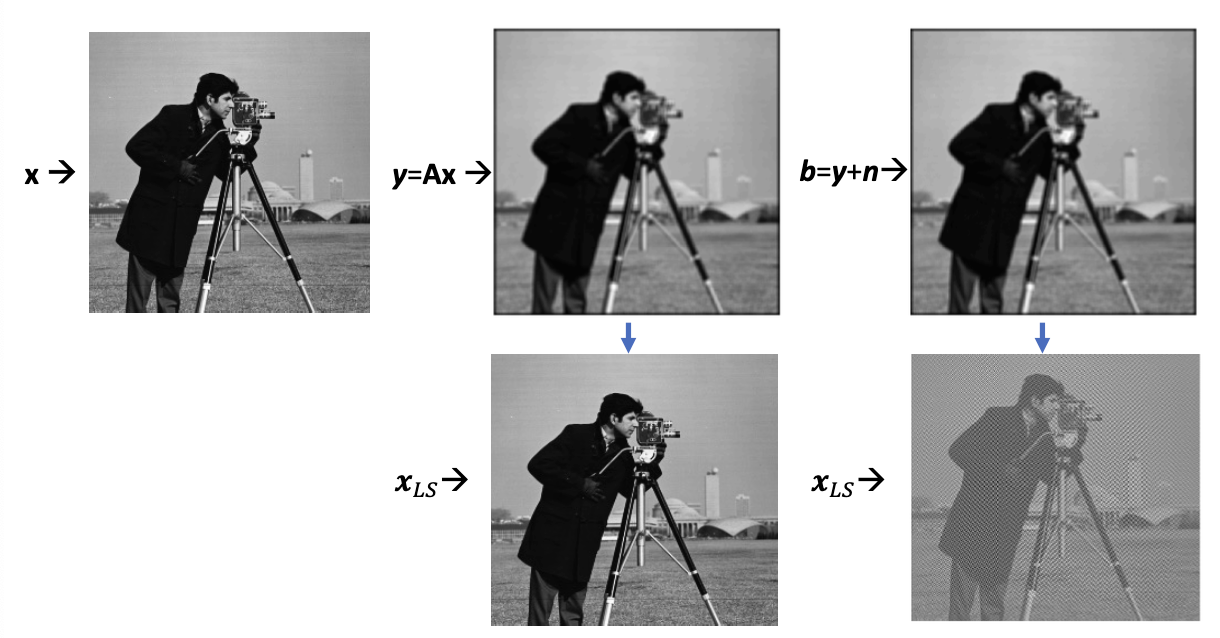
\includegraphics[width=0.75\linewidth]{img/ls-deconv.png}
    \caption{Some noise does end up back in the Least-Squares solution.}
    
\end{figure}
\begin{figure}[H]
    \centering
    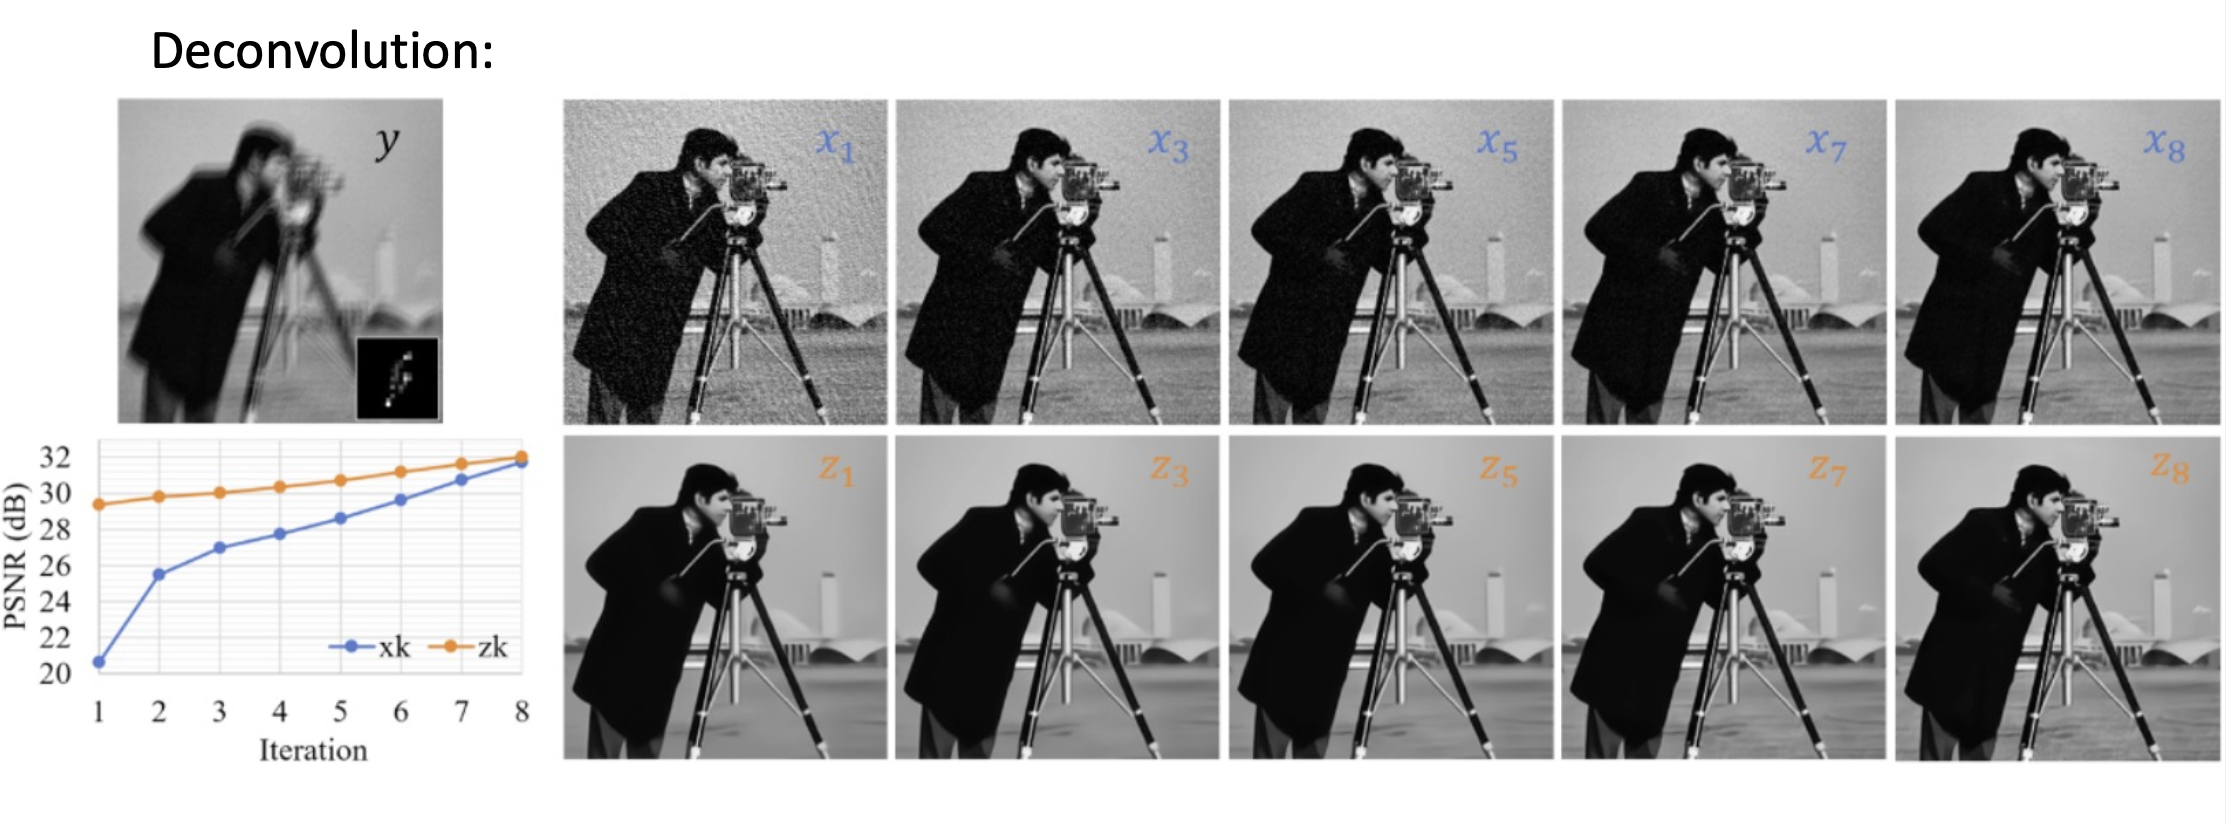
\includegraphics[width=1\linewidth]{img/deconv2.png}
    \caption{Enter Caption}
\end{figure}
\subsection{Example: High-Order Regression}
\textit{(Incomplete)}
% \subsection{Example: Least-Square Deconvolution}
\subsection{Solution (Full Row-Rank Case)}
\begin{itemize}
    \item We now understand how to find an approximate solution \(\textbf{Ax = b}\) in the full column rank case where a solution might exist.
    \item We now consider the full row rank case where \(\textbf{A}\) is fat and we know at least one solution exists.
    \item When the solution exists but is not unique, the set of all solutions has a special structure.
    \item Let \(\textbf{x}_p\) be a solution to \(\textbf{Ax}\textbf{b}\). Then any other solution is \[
    \textbf{x} = \textbf{x}_p
 + \textbf{z}\]
 where \(\textbf{z} \in \mathcal{N}(\textbf{A})    \).
    \item Then the solution to \(\textbf{Ax = b}\) is \(S = \{\textbf{x}_p\} + \mathcal{N}(\textbf{A})\) where \(S\) is a translated subspace of \(\mathcal{N}(\textbf{A)}\) also known as an \textbf{affine subspace}.
    \item We want to pick one of the infinitely many solutions – we look for the \textbf{minimum norm solution}: 
    \[ \min_{||\textbf{x}||} \textbf{Ax} = \textbf{b}\]
\end{itemize}

% \begin{examplebox}{Minimum Norm Solution Example}
%     \begin{itemize}
%         \item Let $\textbf{A} = [1,1]$  and suppose $\textbf{b} = 3$.
%         \item The set of all possible real solutions to $\textbf{Ax} = \textbf{b}$ is defined as $T = \{\textbf{x} : x_1 + x_2 =3  \}$ 
%         \item So $\textbf{x} = \begin{pmatrix}
%             \alpha \\ 3-\alpha 
%         \end{pmatrix} $ and $||x||^2 = \alpha ^2 + (3-\alpha^2)$
%         \item Taking the derivative of the norm and setting it to zero, we find the minimum norm solution \textbf{x}: \[\textbf{x} = \begin{pmatrix}
%             3/2 \\ 3/2
%         \end{pmatrix}\]
%     \end{itemize}



% \centering
% \begin{tikzpicture}[scale=1]
% % Coordinate system
% \draw[thick,->] (-3,0) -- (5,0) node[anchor=south] {$x_1$};
% \draw[thick,->] (0,-3) -- (0,5) node[anchor=west] {$x_2$};

% % Lines with arrows on both ends
% \draw[blue, thick, <->] (-2,-2) -- (3,3) node[anchor=south west] {$\mathcal{N}(A)^\perp$};
% \draw[blue, thick, <->] (-2,2) -- (2,-2) node[anchor=south east] {$\mathcal{N}(A)$};

% % Additional diagonal line
% \draw[blue, thick, <->] (3,-2) -- (-2,3) node[anchor=north] {};

% % Points and labels for the minimum norm solution
% \node[label={[label distance=0.5em]45:{$x_{MN}$}},circle,fill,inner sep=2pt] at (0.5,0.5) {};
% \node[anchor=south west] at (1,0.5) {$\left(\frac{3}{2},\frac{3}{2}\right)$};

% % Annotations
% \node[anchor=north, align=center] at (2.5,-2.5) {$S = \{ x \in \mathbb{R}^2 :$\\$ x_1 + x_2 = 3 \}$};
% \node[anchor=south, align=center] at (-2.5,2.5) {$\mathcal{N}(A) = \{ x \in \mathbb{R}^2 :$\\$ x_1 + x_2 = 0 \}$};

% \end{tikzpicture}




% \end{examplebox}

\begin{theorembox}{Dual Projection Theorem (without proof)}
Let \( T = \{x_p\} + S \) be an affine subspace of \( \mathbb{C}^n \). \\

Then the element \( t_{MN} \) of \( T \) with minimum norm exists, is unique, and satisfies \( t_{MN} \in T \cap S^{\perp} \).\\

Moreover, \( t_{MN} = P_{S^{\perp}}t \).\\

First, observe that the affine subspace \( T \) can be expressed as a translation of the subspace \( S \) by the vector \( x_p \). This translation does not affect the property of orthogonality, so the orthogonal complement of \( S \) is the same as the orthogonal complement of \( T \).\\

The existence and uniqueness of \( t_{MN} \) follow from the properties of Hilbert spaces. Specifically, since \( \mathbb{C}^n \) with the standard inner product is a Hilbert space, there exists a unique element of minimal norm in the closure of the convex set \( T \). The element \( t_{MN} \) is the projection of the origin onto the convex set \( T \), which exists and is unique due to the Hilbert space projection theorem.\\

To show that \( t_{MN} \in T \cap S^{\perp} \), we use the fact that for any \( t \in T \), the difference \( t - t_{MN} \) is orthogonal to \( S^{\perp} \) because the projection onto a closed convex set is the nearest point in the set to the origin, and all other points in \( T \) must be further away.\\

Finally, \( t_{MN} = P_{S^{\perp}}t \) because the projection operator \( P_{S^{\perp}} \) is idempotent and self-adjoint, meaning that \( P_{S^{\perp}} \) applied to any \( t \in T \) yields the unique closest point in \( T \cap S^{\perp} \), which is \( t_{MN} \).\\

Therefore, \( t_{MN} \) is the minimum norm element of \( T \), it is unique, and it lies in both \( T \) and \( S^{\perp} \).
\\
\end{theorembox}

\begin{theorembox}{Minimum Norm Theorem}
Let \( \textbf{Ax} = \textbf{b} \) and let \( A \) be a full-row rank matrix.\\
Amongst all the \( x \in \mathbb{C}^n \) satisfying \( \textbf{Ax} = \textbf{b} \), there exists a unique solution with minimum norm. It lies in \( \mathcal{R}(A^H) \) and is given by \( \textbf{x}_{MN} = \textbf{A}_{MN}b \) with \( \textbf{A}_{MN} = \textbf{A}^\textbf{H}(\textbf{AA}^\textbf{H})^{-1} \).\\

If \( \textbf{x}_p \) is a solution to \( \textbf{Ax} = \textbf{b} \) then all the solutions are in the affine subspace \( T = \{\textbf{x}_p\} + \mathcal{N}(A) \). \\

Using the Dual Projection Theorem we conclude that \[ x_{MN} \in T \cap \mathcal{N}(A)^{\perp} = T \cap \mathcal{R}(A^H) \] \\

Since \( x_{MN} \in \mathcal{R}(A^H) \) implies \( x_{MN} = A^Hz \) and hence \( b = Ax_{MN} = (AA^H)z \).\\

Therefore, \( z = (AA^H)^{-1}b \) which implies that \( x_{MN} = A^H(AA^H)^{-1}b \).
\end{theorembox}

\section{Computing Left and Right Inverses}
\subsubsection*{Claim:}
Assume $\textbf{A}$ is tall, full-column rank, then $\textbf{A}$ has a left inverse $\textbf{A}_{left}$

\subsubsection*{Sketch of Proof:}
$\textbf{A}^\top \textbf{A}$ is full rank, so $(\textbf{A}^\top \textbf{A})^{-1}$ exists. Then $\textbf{A}_{left} = (\textbf{A}^\top \textbf{A})^{-1} \textbf{A}^\top$ 

\subsubsection*{Likewise:}
Assume $\textbf{A}$ is fat and full-row rank, then \textbf{A} has right invese $\textbf{A}_{right}$ and $\textbf{A}_{right} = \textbf{A}^\top (\textbf{AA}^\top)^{-1}$

\section{Least-Square Problems with Linear Constraints}
Revisiting the minimum norm solution approach – we recall that in the full row-rank case, at least one solution exists. Since there are infinitely many solutions, we look for a specific one:

\[\min||x||^2 \text{subject to } \textbf{Ax}=\textbf{b}\]

We can interpret the equation above differently as a least-squares minimisation with linear constraints.

\[x=\begin{pmatrix}
    x_1\\x_2\\ \vdots \\ x_n
\end{pmatrix}
b=\begin{pmatrix}
    b_1\\b_2\\ \vdots \\ b_n
\end{pmatrix}
\]

% (what diagram did he use in the slide????)

\[\min||\textbf{y}-\textbf{Cx}||^2 \text{subject to } \textbf{Ax}=\textbf{b}\]

To solve this constrained optimisation problem, we introduce the method of Lagrangian multipliers. The Lagrangian function is given by:
\[
L(\mathbf{x}, \boldsymbol{\lambda}) = \|\mathbf{y} - \mathbf{C}\mathbf{x}\|^2 + \sum_{i=1}^{m} \lambda_i (\mathbf{a}_i^\mathsf{T}\mathbf{x} - b_i),
\]
where $\mathbf{a}_i^\mathsf{T}$ are the rows of $\mathbf{A}$ and $\lambda_i$ are the Lagrangian multipliers associated with each constraint.

\[
L(\mathbf{x}, \boldsymbol{\lambda}) = (\mathbf{y} - \mathbf{C}\mathbf{x})^\mathsf{T}(\mathbf{y} - \mathbf{C}\mathbf{x}) + \boldsymbol{\lambda}^\mathsf{T}\mathbf{A}\mathbf{x} - \boldsymbol{\lambda}^\mathsf{T}\mathbf{b}.
\]


To find the minimum, we take the gradient of the Lagrangian with respect to $\mathbf{x}$ and set it to zero:
\[
\frac{\partial L(\mathbf{x}, \boldsymbol{\lambda})}{\partial \mathbf{x}} = 0 \implies 2\mathbf{C}^\mathsf{T}\mathbf{C}\mathbf{x} - 2\mathbf{C}^\mathsf{T}\mathbf{y} + \mathbf{A}^\mathsf{T}\boldsymbol{\lambda}=\mathbf{0}.
\]

By combining this set of linear equations with the feasibility conditions $\mathbf{A}\mathbf{x} = \mathbf{b}$, we can write the optimality conditions as one set of $m+n$ linear equations in the variables $(\mathbf{x}; \boldsymbol{\lambda})$:
\[
\begin{pmatrix}
2\mathbf{C}^\mathsf{T}\mathbf{C} & \mathbf{A}^\mathsf{T} \\
\mathbf{A} & \mathbf{0}
\end{pmatrix}
\begin{pmatrix}
\mathbf{x} \\
\boldsymbol{\lambda}
\end{pmatrix}
=
\begin{pmatrix}
2\mathbf{C}^\mathsf{T}\mathbf{y} \\
\mathbf{b}
\end{pmatrix}.
\]

Solving this system yields the vector $\mathbf{x}$ that minimises the squared norm while satisfying the constraints.\\

Note that the square matrix $\begin{pmatrix}
2\mathbf{C}^\mathsf{T}\mathbf{C} & \mathbf{A}^\mathsf{T} \\
\mathbf{A} & \mathbf{0}
\end{pmatrix}
\begin{pmatrix}
\mathbf{x} \\
\boldsymbol{\lambda}
\end{pmatrix}$ is invertible iff \textbf{A} is full row rank and $\begin{pmatrix}
    \textbf{C}\\ \textbf{A} 
\end{pmatrix}$ is full column-rank.







\chapter{Pseudoinverses and the SVD}

\section{Singular Value Decomposition}

Singular Value Decomposition is a fundamental technique in Linear Algebra, particularly for dealing with non-square matrices.

\subsection{Diagonalization of a Matrix}
Consider a matrix \( A \) of dimension \( m \times n \) and rank \( r \). To diagonalize \( A \), we usually perform a transformation \( A = S\Lambda S^{-1} \). However, this approach has limitations:
\begin{itemize}
    \item The matrix \( A \) must be square.
    \item There may not be a sufficient number of eigenvectors to form the matrix \( S \).
\end{itemize}

For example, the matrix 
\( \begin{pmatrix}
1 & a \\
0 & 1
\end{pmatrix} \)
with \( a \neq 0 \) has only the eigenvector \( \begin{pmatrix} x & 0 \end{pmatrix} \).

\textbf{Goal:} We seek a type of decomposition that applies to any matrix.

\subsection{The Singular Value Decomposition Theorem}

\textbf{Theorem:}

Every matrix \( A \in \mathbb{C}^{m \times n} \) can be factored as \( A = U\Sigma V^H \), where:
\begin{itemize}
    \item \( U \) is a unitary matrix \( (U^H U = I) \) with columns \( u_i \) and dimension \( m \times m \).
    \item \( \Sigma \) is an \( m \times n \) rectangular matrix with non-negative real entries along the main diagonal.
    \item \( V \) is a unitary matrix \( (V^H V = I) \) with columns \( v_i \) and dimension \( n \times n \).
\end{itemize}


\begin{itemize}
    \item \( U \) is generally different from \( V \).
    \item The elements of \( \Sigma \), called the singular values of \( A \), are positive and typically ordered.
    \item For square invertible matrices, this decomposition is similar to the eigendecomposition.
\end{itemize}

\subsection{Properties of SVD}
\begin{itemize}
    \item If \( m = 2 \) and \( n = 3 \), \( \Sigma \) would look like \( \begin{pmatrix} \sigma_1 & 0 & 0 \\ 0 & \sigma_2 & 0 \end{pmatrix} \).
    \item \( A^H A = V\Sigma^T U^H U\Sigma V^H = V\Sigma^T \Sigma V^H \), indicating \( \sigma_i^2 \) are the eigenvalues of \( A^H A \) and \( V \) contains the eigenvectors.
    \item Similarly, \( AA^H = U\Sigma V^H V\Sigma^T U^H = U\Sigma \Sigma^T U^H \), showing \( \sigma_i^2 \) are the eigenvalues of \( AA^H \) and \( U \) contains the eigenvectors.
    \item The non-zero elements of \( \Sigma \Sigma^T \) and \( \Sigma^T \Sigma \) are identical.
\end{itemize}

% \textbf{Conclusion:} SVD allows us to decompose any matrix into a product of three matrices, capturing the essence of the matrix in terms of its singular values and vectors.

\subsection{More properties of the SVD}

Matrices \( A \), \( A^H A \) and \( AA^H \) have the same rank.

Let \( A \) be an \( m \times n \) matrix with rank \( r \). The matrix \( A \) has \( r \) singular values. Both \( A^H A \) and \( AA^H \) have \( r \) non-zero eigenvalues which are the squares of the singular values of \( A \). Furthermore:
\begin{itemize}
    \item \( A^H A \) is of dimension \( n \times n \). It has \( r \) eigenvectors \( \{v_1, \ldots, v_r\} \) associated with its \( r \) non-zero eigenvalues and \( n - r \) eigenvectors associated with its \( n - r \) zero eigenvalues.
    \item \( AA^H \) is of dimension \( m \times m \). It has \( r \) eigenvectors \( \{u_1, \ldots, u_r\} \) associated with its \( r \) non-zero eigenvalues and \( m - r \) eigenvectors associated with its \( m - r \) zero eigenvalues.
\end{itemize}

We can write \( V = [v_1 \ldots v_r v_{r+1} \ldots v_n] \) and \( U = [u_1 \ldots u_r u_{r+1} \ldots u_m] \).\\

Note that in the above matrices, we put first in the columns the eigenvectors of \( A^H A \) and \( AA^H \) which correspond to non-zero eigenvalues. We usually order the eigenvectors according to the magnitude of the associated eigenvalue, so the eigenvector that corresponds to the maximum eigenvalue is placed in the first column and so on.\\


As already shown, from \( A = U\Sigma V^H \) we obtain that \( AV = U\Sigma \) or \( A[v_1 \ldots v_r v_{r+1} \ldots v_n] = [u_1 \ldots u_r u_{r+1} \ldots u_m]\Sigma \).\\

Therefore, we can break \( AV = U\Sigma \) into a set of relationships of the form \( Av_i = \sigma_i u_i \). Note that \( \sigma_i \) is a scalar and \( v_i \) and \( u_i \) vectors.\\

For \( i \leq r \) the relationship \( AV = U\Sigma \) tells us that:
\begin{itemize}
    \item The vectors \( u_1, u_2, \ldots, u_r \) are in the column space of \( A \). This observation comes directly from \( u_i = \frac{1}{\sigma_i} Av_i, \sigma_i \neq 0 \), i.e., \( u_i \)s are linear combinations of columns of \( A \). Furthermore, the \( u_i \)s associated with \( \sigma_i \neq 0 \) are orthonormal. Thus, they form a basis of the column space.
    \item The vectors \( v_1, v_2, \ldots, v_r \) are in the row space of \( A \). This is because from \( AV = U\Sigma \) we have \( U^H AV^H = U^H U\Sigma V^H \) \( \Rightarrow U^H A = \Sigma V^H \) \( \Rightarrow A^H = V\Sigma^H U^H \) \( \Rightarrow A^H = V\bar{\Sigma} U^H \), where \( \bar{\Sigma} \) is \( \Sigma^H \) with non-zero elements \( \frac{1}{\sigma_i} \), \( \sigma_i \neq 0 \). Furthermore, since the \( v_i \)'s associated with \( \sigma_i \neq 0 \) are orthonormal, they form a basis of the row space.

\end{itemize}

\begin{itemize}
    \item $\textbf{Av}_i = \sigma_i \textbf{u}_i$ 
    \item $\textbf{v}^\top_i = \frac{1}{\sigma_i}\textbf{u}^\top_i\textbf{A} $
    \item $\textbf{v}_i$ forms an orthonormal basis for the row space of \textbf{A}
    \item $\textbf{u}_i$ forms an orthonormal basis for the column space of \textbf{A}
    \item Any extra $n - r$ additional \textbf{v}'s corresponding to zero eigenvalues of $\textbf{A}^H\textbf{A}$ are taken from the null space of \textbf{A}.
    \item Any extra $m - r$ additional \textbf{u}'s corresponding to zero eigenvalues of $\textbf{A}\textbf{A}^H$ are taken from the null space of $\textbf{A}^H$.
\end{itemize}

We split \( [v_1 \quad \ldots \quad v_r \quad v_{r+1} \quad \ldots \quad v_n] = [V_1 \quad V_2] \) and \( [u_1 \quad \ldots \quad u_r \quad u_{r+1} \quad \ldots \quad u_m] = [U_1 \quad U_2] \), it then follows that:

\[A\begin{bmatrix}v_1&...&v_r & v_{r+1} & ...& v_n\end{bmatrix}=\begin{bmatrix}u_1&...&u_r& u_{r+1} & ...& u_m\end{bmatrix}\Sigma\]


\begin{itemize}
    \item \( \mathcal{R}(A) = \text{span}\{U_1\} \),
    \item \( \mathcal{N}(A) = \text{span}\{V_2\} \),
    \item \( \mathcal{R}(A^H) = \text{span}\{V_1\} \),
    \item \( \mathcal{N}(A^H) = \text{span}\{U_2\} \).
\end{itemize}

\begin{definitionbox}{Truncated or Reduced Singular Value Decomposition}
We can visualise the $AV = U\Sigma$ as such, ignoring eigenvectors that correspond to zero eigenvalues, making $\Sigma$ a square matrix:
\[A\begin{bmatrix}v_1&...&v_r\end{bmatrix}=\begin{bmatrix}u_1&...&u_r\end{bmatrix}\begin{bmatrix}\sigma_1&\cdots&0\\\vdots&\ddots&\vdots\\0&\cdots&\sigma_r\end{bmatrix}\Rightarrow A=u_1\sigma_1v_1^H+\cdots+u_r\sigma_rv_r^H = A=\sum_{i=1}^r\sigma_i\boldsymbol{u}_i\boldsymbol{v}_i^H\]

\begin{itemize}
    \item The dimension of \( A \) is \( m \times n \).
    \item The dimension of \( [v_1 \quad \ldots \quad v_r] \) is \( n \times r \).
    \item The dimension of \( [u_1 \quad \ldots \quad u_r] \) is \( m \times r \).
    \item The dimension of \( \Sigma \) is \( r \times r \).
\end{itemize}

Which is the form for the Truncated or Reduced Singular Value Decomposition, which is the sum of r rank-one matrices.

\end{definitionbox}


\section{Relating the SVD to the pseudo-inverse}

We now go back to the solution to \( A\mathbf{x} = \mathbf{b} \) when \( A \) is neither full column nor row rank.\\

\textbf{Claim:} The Minimum Norm Least Squares solution to \( A\mathbf{x} = \mathbf{b} \) is given by \( \mathbf{x} = A^+\mathbf{b} \) where \( A^+ \) is the pseudoinverse of \( A = U\Sigma V^H \) and is given by \( A^+ = V\Sigma^+U^H \) where\\

\[\mathbf{\Sigma}^{+}=\begin{pmatrix}\frac{1}{\sigma_{1}}&&&&&\\&\ddots&&&&\\&&\frac{1}{\sigma_{r}}&&&\\&&&0&&\\&&&&&\ddots\end{pmatrix}\]

\textbf{Proof:}
We rewrite our problem as:
\[
\min_{\mathbf{x}} \|A\mathbf{x} - \mathbf{b}\| = \min_{\mathbf{x}} \|U\Sigma V^H\mathbf{x} - \mathbf{b}\| = \min_{\mathbf{x}} \| \Sigma V^H\mathbf{x} - U^H\mathbf{b} \|
\]
where the last equality follows from the fact that \( U \) is unitary.

We denote with \( \mathbf{v} = V^H\mathbf{x} \) and \( \mathbf{\tilde{b}} = U^H\mathbf{b} \) then the least-squares problem reduces to 
\[
\min_{\mathbf{v}} \|\Sigma\mathbf{v} - \mathbf{\tilde{b}}\|
\]
for which we know the solution is \( \mathbf{v} = \Sigma^+\mathbf{\tilde{b}} \).

By working backwards we then find the MNLS solution

\[ V^H\mathbf{\hat{x}} = \Sigma^+U^H\mathbf{b}\]\[\Rightarrow \mathbf{\hat{x}} = V\Sigma^+U^H\mathbf{b} \].

\section{Applications of the SVD}
\subsection{Low Rank Approximation}

Given a matrix \( D \), the goal of a low-rank approximation is to find a matrix \( \tilde{D} \) with rank \( r \) that approximates \( D \). This is particularly useful when \( D \) is noisy, or we know a priori that \( D \) is rank deficient.

\subsubsection*{Frobenius Norm}

To measure the approximation, we use the Frobenius norm. For a matrix \( A \), it is defined as:
\[
\|A\|_F = \left( \sum_{i,j} |a_{i,j}|^2 \right)^{\frac{1}{2}} = \left( \text{trace}(A^HA) \right)^{\frac{1}{2}} = \left( \sum_{i} \sigma_i^2 \right)^{\frac{1}{2}}
\]
where \( \sigma_i \) are the singular values of \( A \).

\subsubsection*{Singular Value Decomposition (SVD)}

The Singular Value Decomposition of \( D \) is given by \( D = U\Sigma V^H \), where \( U \) and \( V \) are unitary matrices, \( \Sigma \) is a diagonal matrix with non-negative real numbers on the diagonal (the singular values), and \( H \) denotes the conjugate transpose.

\subsubsection*{Rank-\( r \) Approximation}

For a rank-\( r \) approximation, we consider:
\[
\tilde{D} = \sum_{i=1}^r \sigma_i u_i v_i^H
\]

We can visualise the \( U\Sigma V^H \) as such, ignoring eigenvectors that correspond to zero eigenvalues, making \( \Sigma \) a square matrix:
\[
D\begin{bmatrix}v_1&\cdots&v_r\end{bmatrix} = \begin{bmatrix}u_1&\cdots&u_r\end{bmatrix}\begin{bmatrix}\sigma_1&\cdots&0\\\vdots&\ddots&\vdots\\0&\cdots&\sigma_r\end{bmatrix} \Rightarrow D = u_1\sigma_1v_1^H + \cdots + u_r\sigma_rv_r^H = \sum_{i=1}^r \sigma_i \bm{u}_i \bm{v}_i^H
\]

\begin{itemize}
    \item The dimension of \( D \) is \( m \times n \).
    \item The dimension of \( [v_1 \quad \cdots \quad v_r] \) is \( n \times r \).
    \item The dimension of \( [u_1 \quad \cdots \quad u_r] \) is \( m \times r \).
    \item The dimension of \( \Sigma \) is \( r \times r \).
\end{itemize}

This is the form for the Truncated or Reduced Singular Value Decomposition, which is the sum of \( r \) rank-one matrices.

\subsection{Principal Component Analysis}
Principal Component Analysis (PCA) is a statistical procedure that uses an orthogonal transformation to convert a set of observations of possibly correlated variables into a set of values of linearly uncorrelated variables called principal components.

\subsubsection*{Data Matrix and Mean Centering}

Consider a data matrix \( X \) with \( n \) columns and \( m \) rows, where the columns represent the number of samples and the rows correspond to \( m \) variables measured for each sample (e.g., height, weight, etc.). The preprocessing step in PCA involves mean centering, where the mean value is removed from each row.

\subsubsection*{Principal Components}

The principal components of the data are selected so that the \( i \)-th principal component is the linear combination of the data that accounts for the \( i \)-th largest portion of the variance of the data.

\subsubsection*{First Principal Component}

The first principal component \( a_1 \) is a linear combination \( y_1^T = a_1^T X \) such that the sample variance of \( y_{1,i} \) is maximised subject to the constraint \( ||a_1|| = 1 \).\\

The sample variance \( \sigma_{y_1}^2 \) is given by:
\[
\sigma_{y_1}^2 = \frac{1}{n-1} \sum_{i=1}^n y_{1,i}^2 = \frac{1}{n-1} \sum_{i=1}^n (a_1^T x_i)^2 = a_1^T S a_1
\]
where \( S \) is the covariance matrix:
\[
S = \frac{1}{n-1} XX^T
\]

Maximising \( a_1^T S a_1 \) subject to \( ||a_1|| = 1 \) leads us to an eigenvalue problem, and the solution is the eigenvector corresponding to the largest eigenvalue of \( S \). This is equivalent to the left singular vector of \( X \) related to its largest singular value.

\subsubsection*{Second Principal Component}

The second principal component \( a_2 \) is chosen so that \( y_2^T = a_2^T X \) is uncorrelated with \( y_1 \), which leads to the constraint \( a_2^T a_1 = 0 \). This vector is the singular vector related to the second largest singular value of \( X \).


\begin{figure}[H]
    \centering
    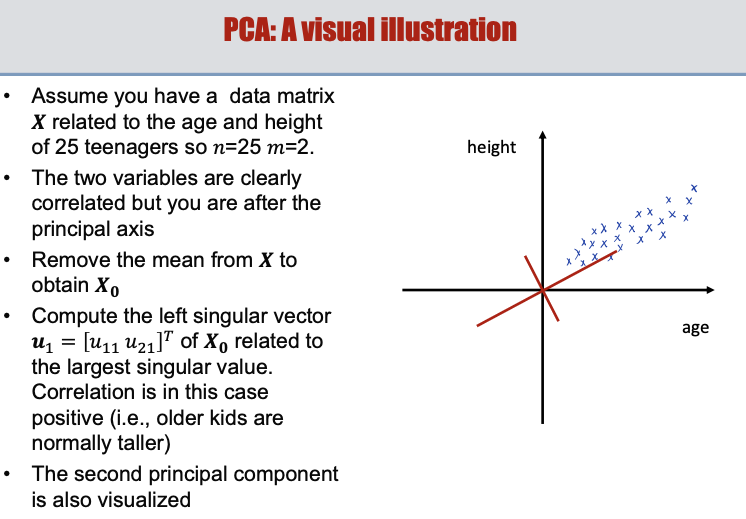
\includegraphics[width=0.75\linewidth]{img/pca-eg.png}
    
    
\end{figure}
\subsection{Total Least Squares}

Let's look again at the minimisation of \(\|A\mathbf{x} - \mathbf{b}\|\) when \( A \) is full column rank. The LS solution essentially finds a \(\mathbf{\tilde{b}}\) such that \(\|\mathbf{b} - \mathbf{\tilde{b}}\|\) is minimised.\\

This is like assuming that \( A \) is noiseless and that the \( \mathbf{b} \) we observe has been corrupted by noise. The \( \mathbf{x} \) we find is the solution to \( A\mathbf{x} = \mathbf{b} + \mathbf{r} \) where \( \mathbf{r} \) is a perturbation we want to minimise.\\

In some cases both \( A \) and \( \mathbf{b} \) are corrupted by noise.\\

We then want to find a solution to the perturbed equation: \( (A + E)\mathbf{x} = \mathbf{b} + \mathbf{r} \). It turns out that this solution is found by using the SVD.\\

Another way to look at the problem is to find the solution $a,b$ to the line $ax + by = 0$. This line minimises the perpendicular distance between the datapoints and the line\\


\begin{figure}[H]
    \centering
\begin{tikzpicture}
\begin{axis}[
    axis lines=middle,
    xlabel=$x$,
    ylabel=$y$,
    xmin=-1, xmax=5,
    ymin=-1, ymax=5,
    xtick={0,1,2,3,4},
    ytick={0,1,2,3,4},
    xticklabels={,,},
    yticklabels={,,},
    clip=false
]

% The line equation y = mx (through the origin)
\addplot [domain=-1:5, samples=2, blue] {x} node[pos=1.1] {$ax + by= 0$};

% Points
% \addplot[mark=*, red] coordinates {(1,2) (3,2) (4,3)};

\node[label={180:{(1,2)}},circle,fill,inner sep=2pt] at (axis cs:1,2) {};
\node[label={0:{(3,2)}},circle,fill,inner sep=2pt] at (axis cs:3,2) {};
\node[label={0:{(4,3)}},circle,fill,inner sep=2pt] at (axis cs:4,3) {};

% Perpendicular lines
\draw[dashed, red] (axis cs:1,2) -- (axis cs:1.42,1.42);
\draw[dashed, red] (axis cs:3,2) -- (axis cs:2.6,2.6);
\draw[dashed, red] (axis cs:4,3) -- (axis cs:3.6,3.6);

\end{axis}
\end{tikzpicture}
\end{figure}



\textbf{When the solution exists is given by:}
\begin{enumerate}
    \item Compute the SVD \([A \quad \mathbf{b}] = U\Sigma V^H\)
    \item Then \(\mathbf{\hat{x}} = -v_{n+1}(1:n)/v_{n+1}(n + 1)\)
\end{enumerate}

\textbf{Sketch of the proof:}
\begin{itemize}
    \item We write \(A\mathbf{x} = \mathbf{b}\) in homogeneous form: \(C\mathbf{y}=0\) with $C$ being an augmented matrix of dimensions $m \times (n+1)$.
    \item \(C = [A \quad \mathbf{b}] \) and \(\mathbf{y} = \begin{bmatrix}\mathbf{x} \\ -1\end{bmatrix}\)
    \item This evaluates to $A\textbf{x} - b = 0$. $A$ is our matrix data columns, in this case it has 2 columns, one for datapoints' x-coordinates and y-coordinates.
\end{itemize}
For a given matrix \( A \) of size \( m \times n \) with \( m \geq n \), the Singular Value Decomposition is given by \( A = U\Sigma V^H \), where:

\begin{itemize}
    \item \( U \) is an \( m \times m \) unitary matrix,
    \item \( \Sigma \) is an \( m \times n \) rectangular diagonal matrix with non-negative real numbers on the diagonal (the singular values),
    \item \( V \) is an \( n \times n \) unitary matrix,
    \item \( V^H \) is the conjugate transpose of \( V \).
\end{itemize}

Our minimisation problem is 
\[\min_{\mathbf{y}}\|C\mathbf{y}\|^2 \text{ such that } \|\mathbf{y}\| \neq 0\]

Because our formulation is $ax + by = 0$, a and b are relative to each other, so we can assume that they have a magnitude of 1, $\sqrt{a^2 + b^2} = 1$.\\

Then our Lagrangian becomes:
\begin{align*}
    \mathcal{L}(\textbf{y}, \lambda)&= ||C\textbf{y}||^2 + \lambda(||\textbf{y}||^2 -1)\\
    \frac{\partial \mathcal{L}}{\partial \textbf{y}} &= 2C^H C \textbf{y} + 2 \lambda \textbf{y} = 0\\
    &\Rightarrow C^H C \textbf{y} = -\lambda \textbf{y}
\end{align*}

From this we see that \textbf{y} is an eigenvector of $C^H C$.

\begin{align*}
    \mathcal{L}(\textbf{y}, \lambda)&= ||C\textbf{y}||^2 + \lambda(||\textbf{y}||^2 -1)\\
    \frac{\partial \mathcal{L}}{\partial \lambda} &= ||\textbf{y}||^2 - 1 = 0 \\
    &\Rightarrow  \textbf{y}^H\textbf{y} = 1
\end{align*}

We combine our result from the partial derivative of \textbf{y}, and we get this result:

\begin{align*}
    C^H C \textbf{y} &= -\lambda \textbf{y}\\
    \textbf{y}^H  C^H C \textbf{y} &= -\lambda \textbf{y}^H \textbf{y}\\
    (C \textbf{y})^H C \textbf{y} &= -\lambda\\
    ||C \textbf{y} || &= -\lambda
\end{align*}

From this we see \textbf{y} is a minimal eigenvalue-eigenvector pair.





\begin{itemize}
    % \item We try to find \(\min_{\mathbf{y}}\|C\mathbf{y}\|^2\) such that \(\|\mathbf{y}\| \neq 0\)
    % \item We use Lagrangian multipliers to solve this constrained minimisation: \(J = \mathbf{y}^H C^H C \mathbf{y} - \lambda\mathbf{y}^H\mathbf{y}\)
    % \item Taking the gradient with respect to \(\mathbf{y}\) and equating to zero yields \(C^H C\mathbf{y} = \lambda\mathbf{y}\)
    \item The solution is in the direction of the eigenvector corresponding to smallest eigenvalue of \(C^H C\), this is equivalent to the column of \(V\) corresponding to smallest singular value: \(\mathbf{y} = v_{n+1}\)
    \item The solution vector \( \textbf{y} \) aligns with the eigenvector associated with the smallest eigenvalue of \( C^H C \), which is the column of \( V \) corresponding to the smallest singular value. Therefore, \( \textbf{y} = v_{n+1} \).
    \item To determine the solution \( \hat{\textbf{x}} \), we extract the relevant components from \( v_{n+1} \).
    \begin{equation}
        \bm{x} = -\frac{1}{v_{n+1}(n+1)} 
        \begin{bmatrix}
            v_{n+1}(1) \\
            v_{n+1}(2) \\
            \vdots \\
            v_{n+1}(n)
        \end{bmatrix}
    \end{equation}
    where \( v_{n+1}(i) \) denotes the \( i \)-th element of vector \( v_{n+1} \).
        \item In order to find \( \mathbf{x} \) we rescale \( v_{n+1} \) properly and we arrive at the solution \(\mathbf{\hat{x}} = -v_{n+1}(1:n)/v_{n+1}(n + 1)\)

\end{itemize}
When considering the augmented matrix \( [A \quad \mathbf{b}] \), which is formed by appending the vector \( \mathbf{b} \) as an additional column to \( A \), the matrix now has a size of \( m \times (n+1) \). The SVD of this augmented matrix is represented as:

\[ C =[A \quad \mathbf{b}] = U' \Sigma' V'^H \]

\[[A \quad \mathbf{b}]\begin{bmatrix}v_1&...&v_r & v_{r+1} & ...& v_n & v_{n+1}\end{bmatrix}=\begin{bmatrix}u_1&...&u_r& u_{r+1} & ...& u_m\end{bmatrix}\Sigma\]

The dimensions and properties of the matrices in the SVD of the augmented matrix are:

\begin{itemize}
    \item \( U' \) is an \( m \times m \) unitary matrix, similar to \( U \) in the SVD of \( A \),
    \item \( \Sigma' \) is an \( m \times (n+1) \) rectangular diagonal matrix, extended from \( \Sigma \) to accommodate the augmented column,
    \item \( V' \) is an \( (n+1) \times (n+1) \) unitary matrix. The last column of \( V' \), denoted \( v_{n+1} \), is vital for this computation.
\end{itemize}

\begin{figure}[H]
    \centering
    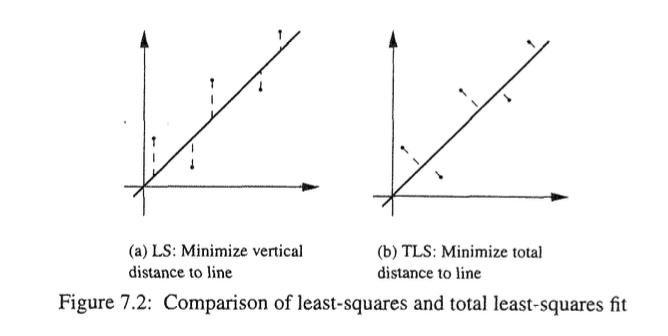
\includegraphics[width=0.75\linewidth]{img/tlsvsls.png}
    
    
\end{figure}

\subsection{Kaczmarz Algorithm}
The Kaczmarz algorithm, also known as the Algebraic Reconstruction Technique (ART) in some contexts, is an iterative method for solving linear systems of equations. Its particular strength is in solving overdetermined systems, which are systems with more equations than unknowns.\\

The algorithm iteratively projects a solution estimate onto the solution set of each equation, one at a time, and repeats this process until convergence to a close-enough solution of linear equations \( A\mathbf{x} = \mathbf{b} \). The procedure is as follows:

\begin{enumerate}
    \item Initialise with any vector \( \mathbf{x}_0 \in \mathbb{R}^n \).
    \item For \( k = 1, 2, \dots, \text{iter} \):
    \begin{itemize}
        \item Compute the next estimate \( \mathbf{x}_{k+1} \) by projecting \( \mathbf{x}_k \) onto the hyperplane defined by the \( i \)-th equation, where \( i = k \mod m + 1 \):
        \[ \mathbf{x}_{k+1} = \mathbf{x}_k + \frac{b_i - \mathbf{a}_i^T \mathbf{x}_k}{\|\mathbf{a}_i\|^2} \mathbf{a}_i \]
    \end{itemize}
    \item Repeat until convergence.
\end{enumerate}

Here, \( \mathbf{a}_i^T \) is the transpose of the \( i \)-th row of matrix \( A \) and represents a hyperplane in \( n \)-dimensional space. The term \( \frac{b_i - \mathbf{a}_i^T \mathbf{x}_k}{\|\mathbf{a}_i\|^2} \) computes the orthogonal projection of the residual \( \mathbf{r}_k = b_i - \mathbf{a}_i^T \mathbf{x}_k \) onto the hyperplane. This process geometrically "corrects" \( \mathbf{x}_k \) in the direction of the \( i \)-th row vector \( \mathbf{a}_i \), moving it closer to the solution with each iteration.
\subsubsection*{Analysis of the Approximation Error}
\begin{enumerate}
    \item Assume \( \bm{x}^* \) is the correct solution to \( A\bm{x} = \bm{b} \).
    \item At the \( (k+1) \)-th iteration, the approximation error is given by:
    \[ \bm{x}_{k+1} - \bm{x}^* = \bm{x}_k - \bm{x}^* + \frac{b_i - \bm{a}_i^T \bm{x}_k}{\| \bm{a}_i \|^2} \bm{a}_i \]
    where \( \bm{a}_i \) is the \( i \)-th row of \( A \), and \( b_i \) is the \( i \)-th component of \( \bm{b} \).
    \item To iterate, we replace \( b_i \) with \( \bm{a}_i^T \bm{x}^* \), obtaining:
    \[ \bm{x}_{k+1} - \bm{x}^* = \left( \bm{x}_k - \bm{x}^* \right) - \frac{\bm{a}_i \bm{a}_i^T}{\| \bm{a}_i \|^2} \left( \bm{x}_k - \bm{x}^* \right) \]
    \item The term \( \frac{\bm{a}_i \bm{a}_i^T}{\| \bm{a}_i \|^2} \left( \bm{x}_k - \bm{x}^* \right) \) represents the projection of the error \( \bm{x}_k - \bm{x}^* \) onto the direction of \( \bm{a}_i \).
    \item Removing the projection of the error along \( \bm{a}_i \) ensures that the error in the direction of \( \bm{a}_i \) is reduced, thus the method makes progress towards convergence.
    \item At each iteration, the norm of the error does not increase:
    \[ \| \bm{x}_{k+1} - \bm{x}^* \| \leq \| \bm{x}_k - \bm{x}^* \| \]
    This inequality shows that the Kaczmarz algorithm is convergent.
\end{enumerate}

\section{Summary}
\begin{table}[h]
\centering
\begin{tabular}{ | m{4cm} | m{3cm} | m{4cm} | m{4.5cm} | }
\hline
\textbf{Scenario} & \textbf{Number of exact Solutions} & \textbf{Type of Solution} & \textbf{Solution} \\
\hline
\( A \) ‘tall’ and full column rank & 0 or 1 & Least square: \( \min\limits_{\mathbf{x}} \|\mathbf{Ax} - \mathbf{b}\| \) & \( \mathbf{x}_{ls} = (A^HA)^{-1}A^H\mathbf{b} \) \\
\hline
\( A \) ‘fat’ and full row rank & Infinitely many solutions & Minimum-norm solution: \( \min\limits_{\mathbf{x}} \|\mathbf{x}\| \) subject to \( A\mathbf{x}=\mathbf{b} \) & \( \mathbf{x}_{MN} = A^H(AA^H)^{-1}\mathbf{b} \) \\
\hline
\( A \) neither full row nor full column rank & 0 or infinitely many solutions & Minimum-norm least square solution & \( \mathbf{\hat{x}} = V\mathbf{\Sigma}^+U^H\mathbf{b} \) with \( A = U\mathbf{\Sigma}V^H \) \\
\hline
\( A \) square and full rank (trivial) & 1 & Unique exact solution & \( \mathbf{x} = A^{-1}\mathbf{b} \) \\
\hline
\end{tabular}
\caption{Solutions to Linear Systems Based on Matrix Structure}
\end{table}

\begin{table}[h!]
\centering
\begin{tabular}{>{\centering\arraybackslash}m{1.5cm} >{\centering\arraybackslash}m{2cm} >{\centering\arraybackslash}m{4cm} >{\centering\arraybackslash}m{2cm} >{\centering\arraybackslash}m{2cm} >{\centering\arraybackslash}m{3cm}}
\toprule
\textbf{Form} & \textbf{Condition} & \textbf{Description} & \textbf{Inverse} & \textbf{Powers} & \textbf{Notes} \\
\midrule
\( S \Lambda S^{-1} \) & Diagonalisable & A matrix is diagonalisable if it can be expressed as the product of an invertible matrix \( S \), a diagonal matrix \( \Lambda \) containing the eigenvalues, and the inverse of \( S \). & \( S \Lambda^{-1} S^{-1} \) & \( S \Lambda^k S^{-1} \) & Suitable for square matrices with \( n \) linearly independent eigenvectors. \\
\addlinespace
\( U \Sigma V^T \) & Any matrix & SVD decomposes any matrix into the product of an orthogonal/unitary matrix \( U \), a diagonal matrix \( \Sigma \) with singular values, and the transpose (or conjugate transpose for complex matrices) of an orthogonal/unitary matrix \( V \). $A^+$ is used for matrices that are not full rank or not invertible. It provides a 'best fit' solution to a system of linear equations. & \( V \Sigma^{-1} U^T \) for invertible \( \Sigma \) (all values on diagonal nonzero) \( A^+ = V \Sigma^+ U^H \) & Generally not defined. & Applicable to all matrices, including non-square ones. When \( A \) is square and full rank, \( V^T = V^{-1} \). $\Sigma^+$ is the reciprocal of values along diagonal, and zero where values are zero. \\
% \addlinespace
% \( A=U \Sigma V^H \) & Non-invertible or rank-deficient & The pseudoinverse $A^+$ is used for matrices that are not full rank or not invertible. It provides a 'best fit' solution to a system of linear equations. & \( A^+ = V \Sigma^+ U^H \). & Not typically computed. & Applicable to any matrix, including non-square ones.  $\Sigma^+$ is the reciprocal of values along diagonal, and zero where values are zero. \\
\addlinespace
\( Q \Lambda Q^T \) & Symmetric Matrices & For symmetric matrices, they can be decomposed into the product of an orthogonal matrix \( Q \), a diagonal matrix \( \Lambda \), and the transpose of \( Q \). & \( Q \Lambda^{-1} Q^T \) & \( Q \Lambda^k Q^T \) & \( Q \) is orthogonal, hence \( Q^T = Q^{-1} \). This is the spectral decomposition. \\
% \addlinespace
% \( R^T R \) & Positive Definite & Cholesky Decomposition is for symmetric and positive definite matrices. It factors the matrix into an upper triangular matrix \( R \) and its transpose. & \( (R^T)^{-1} R^{-1} \) & \( (R^T R)^k \) & Efficient for computational purposes when dealing with positive definite matrices. \\
\addlinespace
\( PA = LU \) & LU Decomposition & The matrix \( A \) is decomposed with the aid of a permutation matrix \( P \), to account for pivoting, into a product of a lower triangular matrix \( L \) and an upper triangular matrix \( U \). &$ A^{-1} = (LU)^{-1}P = U^{-1}L^{-1}P $  &Usually numerically computed  &  For non-integer and negative powers, typically, the LU decomposition is not used; instead, eigenvalue decomposition or other numerical methods are more suitable.\\

\addlinespace
% \( PDP^{-1} \) or \( PDP^* \) & Complex Matrices & For complex matrices that are diagonalisable, they can be decomposed into the product of a matrix \( P \), a diagonal matrix \( D \), and the inverse (or conjugate transpose) of \( P \). & \( PD^{-1}P^{-1} \) or \( PD^{-1}P^* \) & \( PD^kP^{-1} \) or \( PD^kP^* \) & If the matrix is Hermitian (equal to its conjugate transpose), \( P \) is unitary and the decomposition is a form of spectral decomposition. \\
\bottomrule
\end{tabular}
\caption{Matrix Representations and Their Properties}
\label{table:matrix_representations}
\end{table}


\end{document}

